\documentclass[a4paper,oneside]{book}
\usepackage{meccanica-quantistica}

\hypersetup{
	pdftitle={Meccanica Quantistica},
	pdfauthor={Ferracin Davide},
	pdflang={it},
	pdfsubject={Appunti del corso di Meccanica Quantistica},
	pdfcreator={Davide Ferracin},
	pdfcaptionwriter={Davide Ferracin}
	pdfcopyright={Creative Commons Attribution-ShareAlike 4.0 International},
	pdflicenseurl={http://creativecommons.org/licenses/by-sa/4.0/},
	pdfmetalang={it}
}

\title{
	{\sffamily\fontsize{35}{42}\selectfont Meccanica Quantistica}
}
\author{
	{\small a cura di}\\
	Davide Ferracin
}
\date{}

\pagestyle{headings}

\addbibresource{meccanica-quantistica.bib}

\begin{document}
\frontmatter
\maketitle

% Colophon
\null % Serve scrivere qualcosa prima di \vfill altrimenti non funziona
\vfill % Riempie lo spazio verticale della pagina
\hspace*{-1.5em}\includegraphics[scale=.7]{by-sa-icon.pdf}
\begin{flushleft}
	Quest'opera è stata rilasciata con licenza \emph{Creative Commons} Attribuzione - Condividi allo stesso modo 4.0 Internazionale. Per leggere una copia della licenza visita il sito web \url{http://creativecommons.org/licenses/by-sa/4.0/}.\\
	2015, Davide Ferracin (\href{mailto:davide.ferracin@studenti.unimi.it}{\ttfamily davide.ferracin@studenti.unimi.it})\\[1cm]
	Versione aggiornata al \today.
\end{flushleft}

\mainmatter

\chapter{I princ\`ipi della meccanica quantistica}
Vediamo in questo capitolo di porre le fondamenta di questa nuova teoria, inquadrando in una struttura matematica quello che avevamo già visto nell'introduzione, come gli stati, le osservabili e il loro comportamento.
Abbiamo innanzitutto visto la necessità di descrivere gli stati in uno spazio vettoriale, in modo che valga il \emph{principio di sovrapposizione}, e questo stato dovrà essere sul campo complesso per dar luogo a fenomeni di interferenza come nella doppia fenditura.
Lo spazio degli stati, che per ora indichiamo con $\hilbert$, avrà le seguenti proprietà:
\begin{itemize}
	\item è uno spazio vettoriale complesso;
	\item in esso è definito un prodotto scalare definito positivo;
	\item è \emph{completo}, come spazio metrico rispetto alla distanza definita dal prodotto scalare;
	\item è \emph{separabile}, ossia esiste un suo sottoinsieme denso e numerabile;\footnote{Un esempio ``classico'' di spazio separabile è semplicemente $\R$, in cui troviamo $\Q\subset\R$ che è denso e numerabile.} 
\end{itemize}
La completezza implica che tutte le successioni di Cauchy in $\hilbert$ sono anche convergenti, mentre la separabilità assicura l'esistenza di una base ortonormale che abbia cardinalità al più numerabile.
Lo spazio degli stati assuma quindi la struttura di uno \emph{spazio di Hilbert} complesso separabile.

Nella notazione introdotta da Dirac, i vettori di $\hilbert$ sono indicati come \emph{ket}, scritti come $\ket{\cdot}$.
Dobbiamo notare innanzitutto che la corrispondenza tra gli stati fisici e i vettori di questo spazio \emph{non è biunivoca}: mentre un vettore $\ket{x}\in\hilbert$ rappresenta uno e un solo stato fisico, lo stesso stato fisico è rappresentato da $\ket{x}$ e tutti i suoi multipli $\alpha\ket{x}$ per qualsiasi $\alpha\in\C$.
Perciò tutte le informazioni che ricaveremo dal modello quantistico che costruiamo dovranno essere indipendenti da questa arbitrarietà.
Se anzich\'e guardare ai vettori però guardiamo alla classe di vettori che sono tutti multipli (per uno scalare), cioè ai \emph{raggi} dello spazio, allora la corrispondenza diventa s\`i biunivoca.
I ket, quindi, fanno parte di uno spazio vettoriale complesso, dunque ogni combinazione lineare $\alpha\ket{x}+\beta\ket{y}$ è ancora in $\hilbert$.
Possiamo riassumere quanto visto finora nel primo postulato della teoria quantistica.
\begin{postulato}
    Gli stati di un sistema fisico sono descritti da vettori di uno spazio di Hilbert complesso separabile; in particolare, ogni stato è associato a uno e un solo raggio di tale spazio.
\end{postulato}
Il prodotto scalare tra due \emph{ket} è indicato come $\braket{x}{y}$: questa notazione affianca il ket, a destra, con l'elemento a sinistra detto \emph{bra}.
La notazione differente dei due elementi suggerisce una qualche differenza, e in effetti i \emph{ket} e i bra, seppur molto simili, appartengono a due spazi diversi; il prodotto scalare tra due \emph{ket} diventa quindi l'operazione del \emph{bra} associato al primo \emph{ket} sul secondo.
Se i \emph{ket} sono dei vettori di $\hilbert$, possiamo pensare ai \emph{bra} come agli elementi del duale, cioè a funzionali lineari sui ket.
Diamo quindi le proprietà del prodotto scalare cos\`i definito:
\begin{itemize}
	\item è antilineare, ossia $\braket{x}{y}=\braket{y}{x}^*$;
	\item è lineare nella prima variabile, $\braket{x}{\alpha y_1+\beta y_2}=\alpha\braket{x}{y_1}+\beta\braket{x}{y_2}$;
	\item è definito positivo, $\braket{x}{x}\geq 0$ per ogni $\ket{x}\in\hilbert$.
\end{itemize}
Dalle prime due troviamo che è antilineare nella seconda variabile: se vogliamo scomporre il prodotto scalare, dovremo introdurre il coniugato dei componenti, ossia $\braket{\alpha x_1+\beta x_2}{y}=\alpha^*\braket{x_1}{y}+\beta^*\braket{x_2}{y}$.
Dalla terza notiamo infine che il prodotto scalare di un \emph{ket} con se stesso è sempre un numero reale.
Vediamo come costruire questo prodotto scalare: se prendiamo una base ortonormale $\{\ket{e_i}\}$ (quindi $\braket{e_i}{e_j}=\delta_{ij}$), che per semplicità supponiamo finita di cardinalità $n$, allora possiamo esprimere un vettore $\ket{x}$ nei termini di questa base come
\begin{equation}
	\ket{x}=\sum_{i=1}^nx_i\ket{e_i}=x_i\ket{e_i}.
\end{equation}
Analogamente si dà l'espressione di $\ket{y}$, mentre il \emph{bra} associato ad esso è il trasposto coniugato del ket, ossia
\begin{equation}
	\bra{y}=\adj{\ket{y}}=y_i^*\bra{e_i}
\end{equation}
dunque il prodotto scalare tra i due è dato da
\begin{equation}
	\braket{y}{x}=y_j^*x_k\braket{e_j}{e_k}=y_j^*x_k\delta_{jk}=y_j^*x_j,
\end{equation}
che si può anche scrivere come $(y_jx_j^*)^*=\braket{x}{y}^*$, verificando quindi la prima proprietà.

\section{Autovalori e autostati}
Dopo aver inquadrato gli stati del sistema nello spazio di Hilbert con le dovute proprietà, passiamo a studiare le osservabili.
Da un punto di vista prettamente pratico e non matematico possiamo definirle come degli apparecchi che agiscono sul sistema come delle \emph{scatole nere}, di cui non possiamo indagare il funzionamento; successivamente vedremo un modo di definirle anche matematicamente.
Possiamo preoccuparci ora dell'\emph{effetto} che esse producono sul sistema: ad ogni osservabile è associata, chiaramente, una grandezza fisica del sistema, come l'energia, la posizione, eccetera, quindi agendo con un'osservabile sul sistema otteniamo un numero.
Su \emph{come} sia fatto questo numero, però, c'è da discutere.
Sappiamo bene che uno strumento di misura reale ci fornisce una misura con un numero di cifre inevitabilmente finito, quindi questa misura è un numero \emph{razionale}, e il numero di cifre è collegato alla precisione dello strumento.
Possiamo immaginare di aumentare sempre di più questa precisione della misura, ad esempio utilizzando strumenti sempre più sofisticati: nella meccanica classica non si afferma l'esistenza di un limite da porre a questa precisione.
Poich\'e il limite di una successione di numeri razionali è, in generale, un numero reale (dato che $\Q$ non è completo), se aumentiamo indefinitamente la precisione degli strumenti la misura, pur essendo un numero razionale, convergerà ad un numero reale; in effetti la meccanica classica studia i sistemi fisici tramite i numeri reali senza preoccuparsi di questo fatti.

In meccanica quantistica, assumeremo che le osservabili, quindi i nostri strumenti di misura, restituiscano soltanto valori discreti (ma non c'è da preoccuparsi: lo spaziotempo è ancora considerato uno spazio continuo).
Miglioriamo quindi la definizione precedente: diremo che $\xi$ è un'osservabile se è uno ``strumento di misura'' i cui risultati formano un insieme discreto $\{\xi_1,\xi_2,\dots,\xi_n,\dots\}$ (anche infinito).
I valori $\xi_i$ sono detti \emph{autovalori} dell'osservabile $\xi$, e costituiscono quindi i \emph{possibili} risultati della misura.

Torniamo all'esperimento con la lastra polaroid: l'osservabile è la lastra, e il risultato della misura è che il fotone ``passa'' o ``non passa'', e questi due risultati sono quindi gli autovalori.
Associamo al passaggio del fotone l'autovalore 1 e al non passaggio l'autovalore 0.
Non possiamo pretendere di predire il risultato della misura, in generale: sappiamo però che se il fotone è polarizzato linearmente lungo l'asse della lastra, sicuramente passerà, quindi in tale caso avremo con certezza l'autovalore 1.
Analogamente se sappiamo che il fotone è polarizzato ortogonalmente all'asse della lastra, certamente avremo l'autovalore 0.

Più in generale, esistono degli stati del sistema con questa caratteristica: chiamiamo \emph{autostato} un particolare stato del sistema in cui il risultato della misura è certo.
Identificando lo stato con il corrispondente raggio in $\hilbert$, indicheremo con $\ket{\xi_i}$ tale raggio.
Per la corrispondenza biunivoca tra i due elementi, però, spesso chiameremo (impropriamente) stati i raggi di $\hilbert$, per semplificare un poco la notazione.
Indicheremo dunque con $\ket{\xi_i}$ l'autostato dell'osservabile $\xi$ relativo all'autovalore $\xi_i$.
Si ha il seguente postulato.
\begin{postulato}
    Se si misura l'osservabile $\xi$ su un sistema e si ottiene la misura (ossia l'autovalore) $\xi_i$, allora subito dopo tale misura il sistema si troverà in un autostato di $\xi$ corrispondente all'autovalore $\xi_i$.
\end{postulato}
Misurando $\xi$ mentre il sistema è nello stato $\ket{\xi_i}$ siamo certi che otterremo l'autovalore $\xi_i$.
Una volta compiuta la misura, inoltre, abbiamo rimosso ogni incertezza sullo stato attuale del sistema, perch\'e ora lo conosciamo, perciò continuando a misurare la medesima osservabile è chiaro che (almeno negli istanti successivi) otterremo sempre lo stesso risultato,
In generale quindi non ci è dato sapere lo stato del sistema \emph{prima} della misura, ma sapremo in che stato si trova \emph{dopo} averla compiuta: questo è essenzialmente il motivo per cui, compiendo una misura, perturbiamo il sistema.

Prendiamo stavolta due lastre polaroid, allineate lungo lo stesso asse di polarizzazione, e prendiamo gli autovalori 0 e 1 come prima.
Se un fotone passa per le due lastre, è come se misurassimo due volte la sua polarizzazione, quindi rappresentano la stessa osservabile misurata una dopo l'altra.
All'inizio, non sappiamo lo stato del fotone: quando esso passa per la prima lastra, però, può o passare o non passare.
Se passa, cioè se otteniamo 1, il fotone risulta polarizzato lungo l'asse (chiamiamo questo stato $\ket{1}$), quindi certamente passerà anche per la seconda lastra.
Quindi, ricapitolando, misurando il fotone otteniamo 1, dunque siamo sicuri che lo stato del fotone sia $\ket{1}$, che allora passerà anche per la seconda lastra, perch\'e si trova nell'autostato associato all'autovalore 1.
Il discorso è analogo se il fotone non passa attraverso la prima lastra, anche se è una questione un po' delicata perch\'e per la seconda lastra non esiste nemmeno più il fotone da misurare; questo esperimento serve almeno per fissare le idee su questi concetti di base.

Non sempre l'autostato di un autovalore è unico, ma possono esisterne anche di più, anche infiniti: in tal caso, la conoscenza dell'autovalore non determina ancora completamente lo stato del sistema.
Distinguiamo quindi due tipi di osservabili:
\begin{itemize}
	\item quelle \emph{degeneri}, per cui eseguendo la misura non si conosce complessivamente lo stato del sistema (lo è la lastra polaroid: sappiamo la polarizzazione, ma non possiamo conoscere con questo esperiento la frequenza dei fotoni);
	\item quelle \emph{non degeneri}, i cui autovalori determinano completamente lo stato del sistema (corrispondenza biunivoca tra autovalori e stati di $\hilbert$).
\end{itemize}

\section{Probabilità di transizione tra gli stati}
Sappiamo che non possiamo predire il risultato di una misura, a meno che il sistema non sia in un certo autostato: negli altri casi possiamo però sapere la probabilità che un certo risultato si presenti rispetto agli altri.
Il risultato dipenderà quindi sia dallo stato iniziale che da quello di arrivo: cerchiamo ora un metodo per calcolare la probabilità di passare da uno stato $\ket{x}$ allo stato $\ket{y}$.
Questo valore è detto \emph{probabilità di transizione} (dal primo stato all'altro) e lo indicheremo con $P(\ket{x}\to\ket{y})$: esso è dato dal seguente postulato.
\begin{postulato}
    La probabilità di transizione da uno stato $\ket{x}$ a uno stato $\ket{y}$ è data da
    \begin{equation}
        P(\ket{x}\to\ket{y})=\frac{\abs{\braket{x}{y}}^2}{\braket{x}{x}\braket{y}{y}}.
        \label{eq:probabilita-transizione}
    \end{equation}
\end{postulato}
Verifichiamo che è una buona definizione: per cominciare, ci serve un numero reale, quindi prendiamo il prodotto scalare $\braket{x}{y}$ per il suo coniugato, ottenendo $P(\ket{x}\to\ket{y})=\abs{\braket{x}{y}}^2$.
Sicuramente è anche un numero positivo, poich\'e tutti i termini coinvolti nel prodotto lo sono.
Questo però non basta, perch\'e potremmo ottenere un numero maggiore di uno, mentre la probabilità deve essere in $[0,1]$: il denominatore $\braket{x}{x}\braket{y}{y}$ serve dunque a normalizzarla, poich\'e con la disuguaglianza di Schwarz abbiamo $\abs{\braket{x}{y}}^2\leq\braket{x}{x}\braket{y}{y}$ quindi $P(\ket{x}\to\ket{y})\le 1$.
Ciò è equivalente a considerare la probabilità di transizione tra gli stati normalizzati $\braket{x}{x}^{-\frac12}\ket{x}$ e $\braket{y}{y}^{-\frac12}\ket{y}$.\footnote{
    Possiamo trascurare la normalizzazione se assumiamo tutti gli stati normalizzati: questa assunzione è del tutto legittima, poich\'e sappiamo che se $\ket{x}$ rappresenta un certo stato fisico del sistema allora anche $\alpha\ket{x}$ lo rappresenta per qualsiasi $\alpha\in\C$.
}
In particolare, la probabilità è 1 se e solo se il sistema si trova già nello stato ``bersaglio''.
Essa non dipende dal fattore scalare arbitrario nella corrispondenza tra stati fisici e vettori di $\hilbert$: se al posto di $\ket{x}$ e $\ket{y}$ prendiamo $a\ket{x}$ e $b\ket{y}$ per qualunque $a,b\in\C$, abbiamo
\begin{equation}
	P(a\ket{x}\to b\ket{y})=\frac{\abs{a}^2\abs{b}^2\abs{\braket{x}{y}}^2}{\abs{a}^2\braket{x}{x}\abs{y}^2\braket{y}{y}}=\frac{\abs{\braket{x}{y}}^2}{\braket{x}{x}\braket{y}{y}}=P(\ket{x}\to\ket{y}).
\end{equation}
Infine, questa probabilità è simmetrica, cioè $P(\ket{x}\to\ket{y})=P(\ket{y}\to\ket{x})$ come si verifica facilmente scambiando i due ket nella \eqref{eq:probabilita-transizione}.

Prendiamo dunque un'osservabile non degenere $\xi$, e un generico stato $\ket{x}$.
Non sappiamo quale sarà il risultato, ma ogni possibile autovalore $\xi_i$ dell'osservabile avrà una certa probabilità $P_i$ di accadere.
Eseguendo una misura di $\xi$, la probabilità di trovare l'autovalore $\xi_i$ equivale alla probabilità di trovare, dopo la misura, il sistema nell'autostato $\ket{\xi_i}$, quindi è la probabilità di transizione tra $\ket{x}$ e questo autostato:
\begin{equation}
	P_i=\frac{\abs{\braket{\xi_i}{x}}^2}{\braket{\xi_i}{\xi_i}\braket{x}{x}}.
\end{equation}
Ovviamente ogni volta che compiamo la misura dobbiamo ottenere uno degli autovalori, qualunque esso sia, quindi $\sum_kP_k=1$ (gli indici $k$ possono anche essere infiniti).

Se partiamo da un autostato $\ket{\xi_i}$, misurando $\xi$ otterremo sempre con certezza l'autovalore $\xi_i$, quindi la probabilità $P(\ket{\xi_i}\to\ket{\xi_i})$ vale 1.
Come conseguenza abbiamo allora $P(\ket{\xi_i}\to\ket{\xi_k})=0$ per $i\neq k$, dato che la somma di tutte le probabilità è 1, ma allora
\begin{equation}
	P(\ket{\xi_i}\to\ket{\xi_k})=\frac{\abs{\braket{\xi_i}{\xi_k}}^2}{\braket{\xi_i}{\xi_i}\braket{\xi_k}{\xi_k}}=0 \iff \braket{\xi_i}{\xi_k}=0.
	\label{eq:autostati-ortogonali}
\end{equation}
Troviamo allora che
\begin{equation}
	\braket{\xi_i}{\xi_k}=\delta_{ik}
	\label{eq:autostati-ortonormali}
\end{equation}
cioè \emph{due autostati relativi a differenti autovalori sono ortonormali}.

\section{Il postulato di Von Neumann}
Abbiamo dimostrato che gli autostati di un'osservabile non degenere formano un insieme ortonormale.
Esso è anche completo: infatti se esistesse un altro stato $\ket{\phi}$ ortogonale a tutti gli autostati $\ket{\xi_i}$, la probabilità di passare da uno qualunque di questi autostati a $\ket{\phi}$ sarebbe nulla, ma allora $\sum_i\abs{\braket{\xi_i}{\phi}}^2=0$ che è assurdo perch\'e deve essere 1.
Quindi gli autostati (o meglio gli autovettori) di un'osservabile non degenere formano una \emph{base ortonormale} di $\hilbert$.
Chiamiamo \emph{autospazio} relativo all'autovalore $\xi_i$ il sottospazio di $\hilbert$ costituito dagli autostati di tale autovalore.
Se l'osservabile non è degenere, ad ogni autovalore corrisponde un unico autostato, quindi l'autospazio corrispondente ha dimensione 1 (ricordiamo che tutti gli autovettori multipli per uno scalare rappresentano il medesimo stato).
Tutti questi autostati sono anche linearmente indipendenti, in quanto ortonormali, quindi gli autospazi di ciascun autovalore sono tra loro ortogonali (e, ancora, linearmente indipendenti).
Allora detto $\hilbert_i$ l'autospazio dell'autovalore $\xi_i$, possiamo scomporre l'intero spazio $\hilbert$ come somma diretta
\begin{equation}
	\hilbert=\bigoplus_i\hilbert_i.
\end{equation}

Se quindi prendiamo una base di autostati $\{\ket{\xi_i}\}$, possiamo rappresentare ogni stato in termini di questi autostati come
\begin{equation}
	\ket{x}=\sum_ic_i\ket{\xi_i}
\end{equation}
dove i coefficienti $c_i\in\C$ devono soddisfare la condizione $\braket{x}{x}=\sum_ic_i^*c_i=\sum_i\abs{c_i}^2<+\infty$.
Per l'ortonormalità della base possiamo quindi individuare tali coefficienti prendendo il prodotto scalare dello stato $\ket{x}$ con gli autostati, ossia
\begin{equation}
	\braket{\xi_k}{x}=\bra{\xi_k}\sum_ic_i\ket{xi_i}=\sum_ic_i\braket{\xi_k}{\xi_i}=\sum_ic_i\delta_{ik}=c_k,
\end{equation}
ma allora
\begin{equation}
	\ket{x}=\sum_i\braket{\xi_i}{x}\ket{\xi_i}=\sum_i\ket{\xi_i}\braket{\xi_i}{x}=\Big(\sum_i\ket{\xi_i}\bra{\xi_i}\Big)\ket{x}
\end{equation}
da cui ricaviamo che l'operatore $\sum_i\ket{\xi_i}\bra{\xi_i}$ è l'identità su $\hilbert$.
In particolare, il singolo addendo $\ket{\xi_i}\bra{\xi_i}$ è un operatore di \emph{proiezione}, in quanto applicandolo due volte si ha
\begin{equation}
	\ket{\xi_i}\bra{\xi_i}\ket{\xi_i}\bra{\xi_i}=\ket{\xi_i}\braket{\xi_i}{\xi_i}\bra{\xi_i}=\ket{\xi_i}\bra{\xi_i}.
\end{equation}
Inoltre applicandolo ad un vettore si ottiene la sua componente nella direzione di $\ket{\xi_i}$, vale a dire la proiezione di $\ket{x}$ nell'autospazio $\hilbert_i$.
Chiaramente sommando le proiezioni su tutti gli autospazi si ottiene il vettore di partenza, dunque si ha l'operatore identità: questa condizione indica la completezza della base degli autostati.

I discorsi fatti finora valgono solo nel caso di osservabili non degeneri: nell'altro caso, sappiamo che ad un autovalore corrispondono più autostati, che chiaramente dovranno essere linearmente indipendenti (altrimenti rappresenterebbero lo stesso stato fisico).
In questo caso non possiamo sapere in quale autostato si trovi il sistema, ma come al solito possiamo conoscere la probabilità che il sistema si trovi in uno o in un altro.
Per semplicità, consideriamo il caso in cui esistano soltanto di autostati linearmente indipendenti relativi all'autovalore $\xi_1$ di $\xi$: chiamiamo tali autostati $\ket{\xi_1'}$ e $\ket{\xi_1''}$, e assumiamo che gli autovalori $\xi_k$ per $k>1$ non siano degeneri.
Date queste ipotesi allora l'autospazio $\hilbert_1$ ha dimensione 2, ed è chiaramente ortogonale a tutti gli $\hilbert_k$ con $k>1$, quindi anche in questo caso tutti gli $\hilbert_i$ sono linearmente indipendenti e si può scrivere $\hilbert=\bigoplus_i\hilbert_i$.
Possiamo comunque scegliere due vettori linearmente indipendenti da $\hilbert_1$ che insieme agli altri $\ket{\xi_k}$ (sempre $k>1$) formano ancora una base di $\hilbert$; la differenza con le osservabili non degeneri è che ora la base non è più unica, anche a meno di normalizzazioni dei vettori, questo perch\'e in $\hilbert_1$ esistono infinite coppie di vettori linearmente indipendenti anche normalizzati.\footnote{Un caso più ``quotidiano'' analogo a questo lo troviamo nelle basi di $\R$ e di $\R^2$: se consideriamo i vettori a meno di fattori scalari, allora in $\R$ la base può essere una sola (è l'unità) mentre in $\R^2$ ne troviamo infinite, ottenute ruotando la base canonica di un angolo qualsiasi.}

Ad ogni modo, possiamo rappresentare anche in questo caso uno stato $\ket{x}$ in termini della base scelta: abbiamo $\ket{x}=c_1'\ket{\xi_1'}+c_1''\ket{\xi_1''}+\sum_{k>1}c_k\ket{\xi_k}$.
Se abbiamo scelto una base ortonormale, avremo anche in questo caso partendo dallo stato $\ket{x}$ che assumiamo normalizzato, cos\`i come gli autostati, che
\begin{equation}
	\sum_iP_i=\sum_i\abs{\braket{\xi_i}{x}}^2=\sum_i\abs{c_i}^2=\abs{c_1'}^2+\abs{c_1''}^2+\sum_{k>1}\abs{c_k}^2=1,
\end{equation}
dunque per esclusione la probabilità di passare da $\ket{x}$ ad uno stato in $\hilbert_1$ è data da $P_1=1-\sum_{k>1}P_k=1-\sum_{k>1}\abs{c_k}^2=\abs{c_1'}^2+\abs{c_1''}^2$.
Questo discorso è quindi riassunto nel \emph{postulato di Von Neumann}, che afferma
\begin{postulato}
	Se una misura di $\xi$ nello stato $\ket{x}$ risulta nell'autovalore $\xi_i$, allora lo stato dopo al misura è dato dalla proiezione di $\ket{x}$ nell'autospazio di $\xi_i$.
\end{postulato}
Nel caso precedente tale proiezione è proprio $c_1'\ket{\xi_1'}+c_1''\ket{\xi_1''}$, quindi la probabilità di trovare lo stato nell'autospazio $\hilbert_1$ è $\abs{c_1'}^2+\abs{c_1''}^2$.
La probabilità di transizione, dunque, non dipende dalla base scelta per $\hilbert$ (come era lecito aspettarsi).

\section{Osservabili e operatori}
Chiamiamo $E_i$ l'operatore dato da $\ket{\xi_i}\bra{\xi_i}$, con $\xi_i$ autovalore di un'osservabile $\xi$ generica.
Per le proprietà viste in precedenza, $E_i^2=E_i$ perch\'e è una proiezione, inoltre ogni stato si può scrivere come $\ket{x}=\sum_i\ket{\xi_i}\braket{\xi_i}{x}=\sum_iE_i\ket{x}$, se scegliamo gli autostati $\ket{\xi_i}$ in modo da avere una base ortonormale.
Assumiamo $\ket{x}$ e gli autostati della base normalizzati: allora se l'osservabile non è degenere la probabilità $P_i$ di trovare l'autovalore $\xi_i$ è la probabilità di transizione da $\ket{x}$ a $\ket{\xi_i}$, data da
\begin{equation}
	P_i=\abs{\braket{x}{\xi_i}}^2=\braket{x}{\xi_i}\braket{x}{\xi_i}^*=\braket{x}{\xi_i}\braket{\xi_i}{x}=\bra{x}E_i\ket{x}.
	\label{eq:probabilita-proiezione-non-degenere}
\end{equation}
Anche nel caso l'osservabile non sia degenere, il risultato non cambia, se prendiamo comunque la proiezione su ogni vettore della base: per linearità, la proiezione di $\ket{x}$ nell'autospazio è la somma delle proiezioni su ciascun vettore della base che appartiene a tale autospazio.
Più praticamente, riprendendo l'autovalore $\xi_1$ visto in precedenza, e assumendo che esso abbia due autovettori linearmente indipendenti $\ket{\xi_1'}$ e $\ket{\xi_1''}$ ortonormali, allora
\begin{equation}
	P_1=\abs{\braket{x}{\xi_1'}}^2+\abs{\braket{x}{\xi_1''}}^2=\bra{x}E_1'\ket{x}+\bra{x}E_1''\ket{x}=\bra{x}(E_1'+E_1'')\ket{x}.
	\label{eq:probabilita-proiezione-degenere}
\end{equation}

Se compiamo un numero $N$ di misure di $\xi$ sullo stato $\ket{x}$ (ovviamente non possiamo farlo consecutivamente: dobbiamo avere $N$ sistemi tutti nello stesso stato e compiere la misura si ciascuno di essi), misureremo ogni autovalore $\xi_i$ un certo numero $n_i$ di volte, con $\sum_in_i=N$.
Possiamo allora definire il valore medio $\avg{\xi}$ dell'osservabile come
\begin{equation}
	\avg{\xi}=\frac1{N}\sum_in_i\xi_i
	\label{eq:valore-medio-finito}
\end{equation}
e per $N\to+\infty$, cioè con un numero infinito di misure, il rapporto $n_i/N$ tende alla probabilità di trovare $\xi_i$, perciò
\begin{equation}
	\avg{\xi}=\sum_iP_i\xi_i
	\label{eq:valore-medio}
\end{equation}
dove le $P_i$ sono definite come al solito finora.
Se il sistema è nello stato $\ket{x}$, dunque, il valore medio è
\begin{equation}
	\avg{\xi}=\sum_i\xi_i\bra{x}E_i\ket{x}=\bra{x}\sum_iE_i\xi_i\ket{x}.
\end{equation}
Definiamo dunque l'\emph{operatore associato} all'osservabile $\xi$ come
\begin{equation}
	\op{\xi}=\sum_i\xi_iE_i.
	\label{eq:definizione-operatore}
\end{equation}
Si ha dunque, se $\ket{x}$ è normalizzato, che $\avg{\xi}=\bra{x}\op{\xi}\ket{x}$, il quale viene infatti chiamato \emph{valore di aspettazione} dell'osservabile $\xi$ sullo stato $\ket{x}$.

Osserviamo subito che gli operatori associati sono hermitiani, ossia $\adj{\op\xi}=\op\xi$: infatti data una base ortonormale di autostati anche degeneri $\{\ket{\xi_i}\}$ si ha
\begin{equation}
	\bra{x}\op{\xi}\ket{y}=\bra{x}\sum_i\xi_iE_i\ket{y}=\sum_i\xi_i\bra{x}E_i\ket{y}=\sum_i\xi_i\braket{x}{\xi_i}\braket{\xi_i}{y},
\end{equation}
e allo stesso tempo
\begin{equation}
	\bra{x}\adj{\op{\xi}}\ket{y}=\bra{y}\op{\xi}\ket{x}^*=\Big(\sum_i\xi_i\braket{y}{\xi_i}\braket{\xi_i}{x}\Big)^*=\sum_i\xi_i\big(\braket{y}{\xi_i}\braket{\xi_i}{x}\big)^*=\sum_i\xi_i\braket{x}{\xi_i}\braket{\xi_i}{y}
\end{equation}
($\sum_i\xi_i\in\R$ quindi è il coniugato di s\'e stesso) che è dunque uguale a $\bra{x}\op{\xi}\ket{y}$.
Inoltre gli autovalori $\xi_i$, che avevamo definito come i possibili risultati della misura dell'osservabile, sono in realtà anche gli autovalori, nel senso matematico, dell'operatore, perch\'e
\begin{equation}
	\op{\xi}\ket{\xi_i}=\sum_k\xi_kE_k\ket{\xi_i}=\sum_k\xi_k\ket{\xi_k}\braket{\xi_k}{\xi_i}=\sum_k\xi_k\ket{\xi_k}\delta_{ik}=\xi_i\ket{\xi_i}.
\end{equation}

Vediamo due importanti proprietà degli operatori hermitiani:
\begin{itemize}
	\item i suoi autovalori sono tutti reali.
		Se infatti $\op\xi\ket{\xi}=\xi\ket{\xi}$, in generale l'autovalore $\xi$ è complesso, ma in questo caso se moltiplichiamo a sinistra per il \emph{bra} $\bra{\xi}$ otteniamo $\bra{\xi}\op\xi\ket{\xi}=\xi\braket{\xi}{\xi}$, ma $\op\xi=\adj{\op\xi}$ quindi $\bra{\xi}\op\xi\ket{\xi}=\bra{\xi}\adj{\op\xi}\ket{\xi}=\bra{\xi}\op\xi\ket{\xi}^*=(\xi\braket{\xi}{\xi})^*$, ossia
		\begin{equation}
			(\xi\braket{\xi}{\xi})^*=\xi\braket{\xi}{\xi}\quad\then\quad\xi^*=\xi
		\end{equation}
		perch\'e $\braket{\xi}{\xi}\in\R$, ma allora $\xi\in\R$.
	\item gli autospazi corrispondenti a differenti autovalori sono ortogonali.
		Prendiamo due autovalori $\eta'$ e $\eta''$ (ovviamente $\eta'\neq\eta''$) dell'operatore $\op\eta$ hermitiano.
		Prendiamo inoltre l'azione di $\op\eta$ su due autostati corrispondenti ai due autovalori, cioè $\op\eta\ket{\eta'}=\eta'\ket{\eta'}$ e $\op\eta=\eta''\ket{\eta''}$.
		Moltiplicando a sinistra per rispettivamente per $\bra{\eta''}$ e $\bra{\eta'}$ otteniamo
		\begin{equation}
			\begin{cases}
				\bra{\eta''}\op\eta\ket{\eta'}=\eta'\braket{\eta''}{\eta'}\\
				\bra{\eta'}\op\eta\ket{\eta''}=\eta''\braket{\eta'}{\eta''}
			\end{cases}
			\quad\then\quad
			\begin{cases}
				\bra{\eta''}\op\eta\ket{\eta'}=\eta'\braket{\eta''}{\eta'}\\
				\bra{\eta''}\op\eta\ket{\eta'}=\eta''^*\braket{\eta''}{\eta'}
			\end{cases}
		\end{equation}
		ma gli autovalori sono reali quindi nella seconda $\eta''^*=\eta''$.
		Allora sottraendo la seconda equazione dalla prima troviamo
		\begin{equation}
			(\eta'-\eta'')\braket{\eta''}{\eta'}=0
		\end{equation}
		ma se $\eta'\neq\eta''$ allora $\braket{\eta''}{\eta'}=0$, ossia i due autostati sono ortogonali.
\end{itemize}

È dunque vero che tutte le osservabili sono operatori hermitiani?
Per quanto visto finora e per come abbiamo associato gli operatori alle osservabili, s\`i, è vero.
Non è vero però il contrario: sappiamo che con gli autostati di un'osservabile, degenere o meno, possiamo costruire una base ortonormale dello spazio degli stati, ma ciò non è sempre possibile con gli operatori hermitiani.
Se lo spazio $\hilbert$ fosse di dimensione finita, allora per il teorema spettrale ogni operatore hermitiano ammette un insieme di autovettori che forma una base dello spazio, ma questo non è più vero in dimensione infinita.
Alcuni operatori infatti, pur essendo hermitiani, non possiedono abbastanza autovettori linearmente indipendenti da poter costruire una base: gli operatori per cui questo accade, invece, si dicono \emph{autoaggiunti}.
Solo quest'ultimo tipo di operatori corrisponde ad un'osservabile; analogamente tutte le osservabili sono operatori autoaggiunti.

\section{Osservabili compatibili}
Consideriamo due osservabili $\xi$ e $\eta$ sullo stato $\ket{x}$ del sistema.
Misuriamo $\xi$, e lo troviamo in un autostato $\ket{\xi_i}$; se misuriamo ora $\eta$, in generale, non potremo dire niente sul risultato.
Troveremo però il sistema in un autostato $\ket{\eta_j}$: se lo stato precedente $\ket{\xi_i}$ fosse un autostato di $\eta$, allora $\op\eta\ket{\xi_i}=\eta_j\ket{\xi_i}$, quindi la misura non ha alterato il sistema, che rimane nello stesso stato.
Lo stato $\ket{\xi_i}$ è dunque autostato sia di $\xi$ che di $\eta$: se di tali autostati se ne trovano abbastanza da formare una base, le due osservabili si dicono \emph{compatibili}.
\begin{definizione} \label{d:osservabili-compatibili}
	Due osservabili si dicono \emph{compatibili} se ammettono una base di autovettori simultanei.
\end{definizione}
Quindi preso un autostato qualunque, effettuando la misura di un'osservabile compatibile il nuovo stato è ancora un autostato della prima osservabile.

Chiaramente per verificare la compatibilità è impensabile effettuare una misura su tutti gli autostati, che sono infiniti.
Fortunatamente esiste una caratterizzazione di tipo algebrico che permette di verificarlo più semplicemente.
Introduciamo innanzitutto il \emph{commutatore} tra due operatori, definito come
\begin{equation}
	[\op\xi,\op\eta]=\op\xi\op\eta-\op\eta\op\xi.
	\label{eq:commutatore}
\end{equation}
Il risultato del commutatore è a sua volta un operatore, e come anche suggerisce il nome esso fornisce una ``misura'' di quanto gli operatori \emph{non} commutano (e in generale non è nullo).
Le proprietà fondamentali del commutatore sono:
\begin{itemize}
	\item $[\op\eta,\op\xi]=-[\op\xi,\op\eta]$;
	\item per $a,b\in\C$, $[\op\eta,a\op\xi+b\op\lambda]=a[\op\eta,\op\xi]+b[\op\eta,\op\lambda]$;
	\item $[\op\eta,\op\xi\op\lambda]=\op\lambda[\op\eta,\op\xi]+[\op\eta,\op\lambda]\op\xi$.
\end{itemize}
Le prime due sono evidenti dalla definizione del commutatore; per la terza, si ha
\begin{equation}
	\begin{split}
		[\op\eta,\op\xi\op\lambda]&=\op\eta\op\xi\op\lambda-\op\xi\op\lambda\op\eta=\\
		&=\op\eta\op\xi\op\lambda-\op\xi\op\lambda\op\eta+\op\lambda\op\eta\op\xi-\op\lambda\op\eta\op\xi=\\
		&=\op\lambda(\op\eta\op\xi-\op\xi\op\eta)+(\op\eta\op\lambda-\op\lambda\op\eta)\op\xi=\\
		&=\op\lambda[\op\eta,\op\xi]+[\op\eta,\op\lambda]\op\xi.
	\end{split}
\end{equation}
Prima di collegare il commutatore alla compatibilità tra le osservabili, dimostriamo il seguente lemma.
\begin{lemma} \label{l:autostati-compatibili}
	Date due osservabili $\xi$ ed $\eta$, se $[\op\xi,\op\eta]=0$ e $\ket{\xi'}$ è un autostato di $\xi$, allora $\op\eta\ket{\xi'}$ è ancora un autostato di $\xi$ con lo stesso autovalore.
\end{lemma}
\begin{proof}
	Dato che le osservabili commutano, $\op\xi\op\eta\ket{\xi'}=\op\eta\op\xi\ket{\xi'}=\op\eta(\xi'\ket{\xi'})=\xi'\op\eta\ket{\xi'}$, ossia
	\begin{equation}
		\op\xi(\op\eta\ket{\xi'})=\xi'(\op\eta\ket{\xi'}).\qedhere
	\end{equation}
\end{proof}
Questo lemma \emph{non} significa che $\op\eta\ket{\xi'}=\ket{\xi'}$!
Ciò accade soltanto se $\xi$ non è degenere: in tal caso, $\op\eta\ket{\xi'}$ sarebbe un multiplo di $\ket{\xi'}$, ma ricordando che i vettori multipli per uno scalare rappresentano il medesimo stato fisico i due stati sono uguali.
Vediamo dunque come la compatibilità tra due osservabili è legata al loro commutatore, partendo dal caso delle osservabili compatibili; in seguito affronteremo il caso generale.
\begin{teorema} \label{t:osservabili-compatibili}
	Due osservabili $\xi$ e $\eta$ sono compatibili se e solo se $[\op\xi,\op\eta]=0$.
\end{teorema}
\begin{proof}
	Assumiamo le due osservabili compatibili.
	Chiamiamo $\ket{\xi'\eta'}$ uno degli autostati della base in comune, che è tale per cui $\op\xi\ket{\xi'\eta'}=\xi'\ket{\xi'\eta'}$ e $\op\eta\ket{\xi'\eta'}=\eta'\ket{\xi'\eta'}$.
	Ma allora $\op\xi\op\eta\ket{\xi'\eta'}=\op\xi(\op\eta\ket{\xi'\eta'})=\eta'\op\xi\ket{\xi'\eta'}=\eta'\xi'\ket{\xi'\eta'}$, e analogamente $\op\eta\op\xi\ket{\xi'\eta'}=\xi'\eta'\ket{\xi'\eta'}$, quindi $\op\xi\op\eta=\op\eta\op\xi$ su ogni autostato simultaneo.
	Questi autostati, però, formano un insieme completo nonch\'e una base dello spazio, quindi per linearità questo vale pe ogni stato di $\hilbert$.
	Allora $[\op\xi,\op\eta]=0$.

	Partiamo ora da $[\op\xi,\op\eta]=0$, e consideriamo $\xi$ non degenere.
	Se $\ket{\xi_i}$ è un autostato di $\xi$ con autovalore $\xi_i$, allora $\op\eta\ket{\xi_i}$ per il lemma precedente è ancora autostato di $\xi$.
	La dimensione dell'autospazio di tale autovalore però è 1, poich\'e non è degenere, quindi questo nuovo autostato sarà un multiplo del precedente, cioè $\op\eta\ket{\xi_i}=c\ket{\xi_i}$ con $c\in\C$.
	Ma allora $\ket{\xi_i}$ è un autostato di $\eta$.
	Poich\'e questo vale per ogni autostato, e gli autostati di $\xi$ formano già una base, essi sono tutti anche autostati di $\eta$ quindi le due osservabili sono compatibili.

	Prendiamo ora $\xi$ degenere, e assumiamo per semplicità che solo l'autovalore $\xi_1$ sia degenere.
	Possiamo scomporre $\hilbert$ nella somma diretta $\hilbert_1\oplus\hilbert^\perp_1$: il primo termine è l'autospazio dell'autovalore $\xi_1$, il secondo è il suo complemento ortogonale, che è anche la somma dei restanti autospazi (ricordiamo che sono tutti ortogonali tra loro).
	Se $\ket{x}\in\hilbert_1$, per il lemma precedente anche $\op\eta\ket{x}\in\hilbert_1$, perch\'e devono avere lo stesso autovalore di $\xi$.
	Prendiamo un altro stato $\ket{y}$: abbiamo che se $\ket{y}\in\hilbert_1^\perp$ allora $\op\eta\ket{y}\in\hilbert_1^\perp$.
	Infatti $\bra{x}\op\eta\ket{y}=\bra{y}\op\eta\ket{x}^*=0$, perch\'e $\ket{y}$ e $\op\eta\ket{x}$ appartengono a spazi ortogonali, dunque anche $\ket{x}$ e $\op\eta\ket{y}$ appartengono a spazi ortogonali.
	In $\hilbert_1$ possiamo scegliere una base di autostati di $\eta$: essi saranno anche autostati di $\xi$ e avranno lo stesso autovalore, trovandoci nel medesimo autospazio.
	Ripetendo per tutti gli autospazi restanti giungiamo a una base dello spazio degli stati, che è composta da autostati simultanei: ciò prova che le osservabili sono compatibili.
\end{proof}
Anche se il commutatore non è nullo, due osservabili possono comunque avere degli autostati simultanei: certamente non potranno essere abbastanza da formare una base.
Un insieme di osservabili che commutano tra loro, e tali che nessun autovalore sia degenere, formano un \emph{sistema completo di osservabili}; se le prime due presentano ancora delle degenerazioni, si può continuare aggiungendo altre osservabili che commutano fino ad arrivare a un sistema completo.

Con delle osservabili compatibili possiamo inoltre verificare se un'altra osservabile è degenere o meno, con il seguente teorema.
\begin{teorema} \label{t:degenerazione}
	Siano $\xi,\eta,\zeta$ tre osservabili tali che $[\op\xi,\op\eta]=[\op\xi,\op\zeta]=0$ e $[\op\eta,\op\zeta]\ne 0$.
	Allora $\xi$ è degenere.
\end{teorema}
\begin{proof}
	Se $\xi$ non fosse degenere, allora i suoi autostati formerebbero un insieme completo, e coinciderebbero sia con quelli di $\eta$ che con quelli di $\zeta$.
	In tal caso però $\eta$ e $\zeta$ ammetterebbero un insieme completo di autostati simultanei (gli stessi di $\xi$, per transitività) cioè sarebbero compatibili, dunque per il teorema \ref{t:osservabili-compatibili} avremmo $[\op\eta,\op\zeta]=0$ che contraddice le ipotesi.
	Allora $\xi$ deve essere degenere.
\end{proof}

\section{Indeterminazione nella misura}
Come non ci annoiamo mai di ripetere, il risultato della misura di un'osservabile non può essere, in generale, previsto con certezza.
L'unico caso in cui sappiamo che certamente otterremo un dato autovalore è se il sistema si trova nel corrispondente autostato.
Se anche non possiamo conoscere il risultato, però, non significa che la misura darà risultati distribuiti senza criterio: ad esempio, se lo stato $\ket{x}$ del sistema è ``molto vicino'' ad un autostato $\ket{\xi_i}$ dell'osservabile $\xi$, ossia $\abs{\braket{x}{\xi_i}}^2\approx 1$ (prendendo i due stati normalizzati), allora la probabilità di ottenere proprio l'autovalore $\xi_i$ è più alta rispetto a quella di ottenere altri autovalori, e di conseguenza ci aspettiamo che l'indeterminazione nel risultato sia bassa.

Dato uno stato ``di partenza'' $\ket{x}$ del sistema, e in seguito alla misura di $\xi$, sappiamo qual è il valore di aspettazione, ma possiamo anche chiederci come fluttua (statisticamente parlando) il risultato della misura attorno a questo valore.
La quantità più naturale da scegliere a questo scopo è lo \emph{scarto quadratico medio}, che chiamiamo $\Delta_x\xi$, che sarà dunque
\begin{equation}
	\Delta_x\xi=\avg{(\xi-\avg{\xi})^2}=\sqrt{\avg{\xi^2}-\avg{\xi}^2}.
	\label{eq:deviazione-standard}
\end{equation}
Elevando al quadrato, dunque, troviamo
\begin{equation}
	\Delta_x\xi^2=\avg{\xi^2}-\avg{\xi}^2=\bra{x}\op\xi^2\ket{x}-\bra{x}\op\xi\ket{x}^2.
	\label{eq:varianza}
\end{equation}
Guardiamo al quadrato dell'operatore $\op\xi$: esso non è altro che $\op\xi$ applicato consecutivamente, perciò sugli autostati accade che
\begin{equation}
	\op\xi^2\ket{\xi_i}=\op\xi(\op\xi\ket{\xi_i})=\op\xi(\xi_i\ket{\xi_i})=\xi_i\op\xi\ket{\xi_i}=\xi_i^2\ket{\xi_i}
\end{equation}
quindi i suoi autovalori sono il quadrato dei corrispondenti autovalori dell'operatore originario, con i medesimi autostati.

D'altro canto, nella \eqref{eq:deviazione-standard}, $(\xi-\avg{\xi})^2$ è ancora un'osservabile, e possiamo dunque scrivere il suo valore di aspettazione dallo stato $\ket{x}$ come $\bra{x}(\op\xi-\avg\xi)^2\ket{x}$, che a sua volta è esprimibile come\footnote{Rigorosamente, $\avg\xi$ non è un'osservabile n\'e un operatore, ma un numero reale. Possiamo considerarlo tale se supponiamo in realtà $\avg\xi=\avg\xi\op 1$, ossia come multiplo dell'identità, per cui sarebbe anche un operatore autoaggiunto.}
\begin{equation}
	\bra{x}(\op\xi-\avg\xi)^2\ket{x}=\bra{x}(\op\xi-\avg\xi)(\op\xi-\avg\xi)\ket{x}=\bra{x}\adj{(\op\xi-\avg\xi)}(\op\xi-\avg\xi)\ket{x}
\end{equation}
dato che l'operatore $\op\xi-\avg\xi$ che abbiamo introdotto è anch'esso hermitiano, poich\'e $\adj{(\op\xi-\avg\xi)}=\adj{\op\xi}-\adj{\avg\xi}=\op\xi-\avg\xi$.

Possiamo quindi formulare il seguente teorema.
\begin{teorema} \label{t:autostato-indeterminazione-nulla}
	Dato uno stato $\ket{x}$ del sistema e un'osservabile $\xi$, $\Delta_x\xi=0$ se e solo se $\ket{x}$ è un autostato di $\xi$.
\end{teorema}
\begin{proof}
	Se $\Delta_x\xi=0$, allora per quanto abbiamo visto prima $\bra{x}(\op\xi-\avg\xi)(\op\xi-\avg\xi)\ket{x}=0$, ma questo termine è anche la norma del vettore $(\op\xi-\avg\xi)\ket{x}$, che dunque è nullo poich\'e il prodotto scalare non è degenere.
	Allora $(\op\xi-\avg\xi)\ket{x}=0$, vale a dire $\op\xi\ket{x}=\avg\xi\ket{x}$ cioè $\ket{x}$ è un autostato dell'osservabile (con autovalore $\avg\xi$).

	Se invece partiamo dall'ipotesi che $\ket{x}$ sia autostato di $\xi$, allora (chiamiamo $\xi'$ il rispettivo autovalore) $\op\xi=\xi'\ket{x}$.
	Per l'operatore $\op\xi^2$ si ha analogamente $\op\xi^2\ket{x}=\xi'^2\ket{x}$, e moltiplicando a sinistra le due equazioni per $\bra{x}$ otteniamo, supponendo $\ket{x}$ normalizzato,
	\begin{gather}
		\bra{x}\op\xi\ket{x}=\bra{x}\xi'\ket{x}=\xi'\braket{x}{x}=\xi'\\
		\bra{x}\op\xi^2\ket{x}=\bra{x}\xi'^2\ket{x}=\xi'^2\braket{x}{x}=\xi'^2
	\end{gather}
	quindi $\Delta_x\xi^2=\bra{x}\op\xi^2\ket{x}-\bra{x}\op\xi\ket{x}^2=0$.
\end{proof}
Gli autostati dell'osservabile sono quindi gli stati di \emph{minima indeterminazione} del risultato della misura.

In generale sappiamo che due osservabili non commutano, e il loro commutatore fornisce una stima di questo fatto: vediamo come tutto ciò si traduce nell'indeterminazione sulle misure.
\begin{teorema} \label{t:indeterminazione}
	Dato uno stato $\ket{x}$ e due osservabili $\xi$, $\eta$, il prodotto delle due indeterminazioni delle due misure è
	\begin{equation}
		\Delta_x\xi\Delta_x\eta\geq\frac12\abs{\bra{x}i[\op\xi,\op\eta]\ket{x}}.
		\label{eq:indeterminazione}
	\end{equation}
\end{teorema}
\begin{proof}
	Costruiamo l'operatore $\op A=\op\xi+iz\op\eta$, con $z\in\R$: il suo aggiunto è $\adj{\op A}=\adj{\op\xi}-iz\adj{\op\eta}=\op\xi-iz\op\eta$.
	Calcoliamo subito $\adj{\op A}\op A$, che vale
	\begin{equation}
		\adj{\op A}\op A=(\op\xi-iz\op\eta)(\op\xi+iz\op\eta)=\op\xi^2+z^2\op\eta^2-iz\op\eta\op\xi+iz\op\xi\op\eta=\op\xi^2+z^2\op\eta^2+iz[\op\xi,\op\eta].
	\end{equation}
	Assumiamo che lo stato $\ket{x}$ sia normalizzato, e calcoliamo la norma di $\op A\ket{x}$: prendendo una base ortonormale che include $\ket{x}$, l'insieme $\{\op E_i\}$ delle proiezioni sugli elementi della base è tale per cui $\sum_i\op E_i=\op 1$, quindi (possiamo assumere che $\ket{x}$ sia l'elemento della base con indice 1, perciò $E_1$ è la proiezione su $\ket{x}$)
	\begin{equation}
		\begin{split}
			\bra{x}\adj{\op A}\op A\ket{x}&=\bra{x}\adj{\op A}\Big(\sum_i\op E_i\Big)\op A\ket{x}=\\
			&=\sum_i\bra{x}\adj{\op A}\op E_i\op A\ket{x}=\\
			&=\bra{x}\adj{\op A}\op E_1\op A\ket{x}+\sum_{i>1}\bra{x}\adj{\op A}\op E_i\op A\ket{x}=\\
			&=\bra{x}\adj{\op A}\ket{x}\bra{x}\op A\ket{x}+\sum_{i>1}\bra{x}\adj{\op A}\op E_i\op A\ket{x},
		\end{split}
	\end{equation}
	ma tutti gli addendi sono positivi, perch\'e corrispondono a $\big|\bra{e_i}\op A\ket{x}\big|^2$, dove $\ket{e_i}$ sono i vettori della base ortonormale considerata.
	Possiamo quindi sottrarre tutti i termini per $i>1$, ottenendo
	\begin{equation}
		\bra{x}\adj{\op A}\op A\ket{x}\geq\bra{x}\adj{\op A}\ket{x}\bra{x}\op A\ket{x}
	\end{equation}
	I due fattori al secondo membro sono i valori di aspettazione di $\adj{\op A}\op A$	e $\op A$ rispettivamente, quindi dalla definizione di questi operatori troviamo
	\begin{equation}
		\avg{\xi^2}+z^2\avg{\eta^2}+iz\avg{[\xi,\eta]}\geq\avg{(\xi-iz\eta)}\avg{(\xi+iz\eta)}=\avg{\xi}^2+z^2\avg{\eta}^2
	\end{equation}
	e semplificando risulta
	\begin{equation}
		(\avg{\eta^2}-\avg{\eta}^2)z^2+iz\avg{[\xi,\eta]}+\avg{\xi^2}-\avg{\xi}^2\geq 0.
	\end{equation}
	Affinch\'e tale relazione valga per ogni $z\in\R$, il discriminante della forma quadratica deve essere negativo o nullo, quindi $\avg{i[\xi,\eta]}^2-4(\avg{\eta^2}-\avg{\eta}^2)(\avg{\xi^2}-\avg{\xi}^2)=\avg{i[\xi,\eta]}^2-4\Delta_x\xi^2\Delta_x\eta^2\leq 0$, che si riscrive come\footnote{La notazione usata per l'indeterminazione nelle osservabili è da intendersi come un oggetto unico, come il differenziale di una funzione, nel senso che $\Delta_x\xi^2=(\Delta_x\xi)^2$, e non è quindi l'indeterminazione di $\xi^2$ ma il quadrato dell'indeterminazione di $\xi$.}
	\begin{equation}
		\Delta_x\xi\Delta_x\eta\geq\frac12\avg{i[\xi,\eta]}=\frac12\abs{\bra{x}i[\op\xi,\op\eta]\ket{x}}.
	\end{equation}
\end{proof}
Di conseguenza se misuriamo due osservabili su uno stato ed esse non sono compatibili non potremo mai determinarle con assoluta precisione, ma dobbiamo accettare inevitabilmente un'indeterminazione sui risultati.\footnote{La misura delle due osservabili deve essere svolta ``in rapida successione'', nel senso che la seconda deve essere svolta \emph{immediatamente} dopo la prima. Questo perch\'e uno stato non è necessariamente costante nel tempo, ma può evolvere, quindi potremmi trovarci a misurare due osservabili su stati \emph{differenti}, e in tal caso chiaramente questo teorema non si applica più.}
Da questo deriva inoltre il famoso \emph{principio di indeterminazione di Heisenberg}, ad esempio per la coppia di osservabili posizione-impulso.

La presenza di una $i$ nella \eqref{eq:indeterminazione} è dovuta al fatto che il commutatore non è hermitiano, cioè
\begin{equation}
	\adj{[\op\xi,\op\eta]}=\adj{(\op\xi\op\eta-\op\eta\op\xi)}=\adj{\op\eta}\adj{\op\xi}-\adj{\op\xi}\adj{\op\eta}=\op\eta\op\xi-\op\xi\op\eta=-[\op\xi,\op\eta],
	\label{eq:commutatore-antihermitiano}
\end{equation}
quindi non può rappresentare un'osservabile, e il termine $\bra{x}[\op\xi,\op\eta]\ket{x}$ non avrebbe un senso fisico.
Aggiungendo la $i$, come si può verificare facilmente, $i[\op\xi,\op\eta]$ è hermitiano, e automaticamente anche autoaggiunto perch\'e lo sono i due operatori.

\section{Regole di quantizzazione}
Per concludere i principi della meccanica quantistica, volgiamo l'attenzione alle osservabili della meccanica classica.
Avevamo visto che tutte le osservabili sono delle funzioni della posizione $\vec q$ e del momento $\vec p$ (che a loro volta sono delle osservabili).
Anche in meccanica quantistica le osservabili saranno funzioni generiche di posizione e momento, oltre che degli operatori autoaggiunti sullo spazio degli stati; in questo caso però posizione e momento, ossia gli operatori $\op q$ e $\op p$, fanno parte di un'algebra non commutativa, e questo porta ad alcuni cambiamenti.
Ad esempio, passiamo dall'hamiltoniana classica $\ham=\frac1{2m}p^2+\frac{k}2q^2$ all'operatore hamiltoniano semplicemente definendolo come
\begin{equation}
	\op H=\frac1{2m}\op p^2+\frac{k}2\op q^2.
	\label{eq:operatore-hamiltoniano}
\end{equation}
Il problema sorge quando nell'osservabile classica appaiono prodotti di $\vec q$ e $\vec p$, in quanto i corrispondenti operatori non commutano ($\op q\op p\neq\op p\op q$).
Possiamo risolvere questa ambiguità ad esempio sostituendo $\vec q\vec p$ con l'operatore $\frac12(\op q\op p+\op p\op q)$, che è hermitiano.

In generale, quindi, per completare il quadro delle osservabili ci occorre conoscere come ogni coppia di esse commuta, cioè il loro commutatore.
Essendo tutte le osservabili funzioni di $\op q$ e $\op p$, si può vedere che è sufficiente conoscere i commutatori di questi due operatori: le regole di quantizzazione, note anche come \emph{relazioni canoniche di commutazione}, spiegano come questi si comportano.
Dalle proprietà del commutatore, notiamo che tra esso e le parentesi di Poisson esiste una forte relazione algebrica: per questo motivo si postula che
\begin{postulato}
	I commutatori degli operatori di posizione e impulso sono proporzionali alle corrispondenti parentesi di Poisson classiche.
\end{postulato}
Per come sono definiti, le parentesi di Poisson coinvolgono derivate e somme, e hanno come risultato una funzione, mentre il commutatore riguarda semplicemente il prodotto dei due operatori e come risultato dà un altro operatore, quindi non possiamo postulare che i risultati siano i medesimi, ma solo proporzionali: vediamo ora come.
Innanzitutto, siccome $\pois{q_i}{q_j}=0$ e $\pois{p_i}{p_j}=0$, si avrà anche
\begin{equation}
	[\op q_i,\op q_j]=0\quad\text{e}\quad[\op p_i,\op p_j]=0.
\end{equation}
La rimanente parentesi è $\pois{q_i}{p_j}=\delta_{ij}$: non possiamo semplicemente porre $[\op q_i,\op p_j]=\delta_{ij}$ (vale a dire $[\op q_i,\op p_j]=\delta_{ij}\op 1$), poich\'e il commutatore è antihermitiano, cioè $\adj{[\op q_i,\op p_j]}=-[\op q_i,\op p_j]$, ma allora risulterebbe $\adj{\delta_{ij}\op 1}=-\delta_{ij}\op 1$, che è falso perch\'e $\delta_{ij}\op 1$ è chiaramente hermitiano (è un multiplo reale dell'identità).
Dobbiamo allora far s\`i che il risultato di $[\op q_i,\op p_j]$, oltre che multiplo dell'identità, sia anche antihermitiano: lo scalare $z$ per cui moltiplichiamo $\op 1$ deve essere quindi tale che $z^*=-z$.
Questo succede se $z$ è immaginario puro, ossia se $z=ic$ con $c\in\R$.
Allora $[\op q_i,\op p_j]=ic\delta_{ij}$.
La costante $c$ di proporzionalità chiaramente non è ancora ben definita: la chiameremo $\hbar$, senza preoccuparci ora di quanto valga realmente.
I tre commutatori fondamentali sono quindi
\begin{equation}
	[\op q_i,\op q_j]=0\qquad[\op p_i,\op p_j]=0\qquad[\op q_i,\op p_j]=i\hbar\delta_{ij}.
	\label{eq:commutatori-fondamentali}
\end{equation}
Da queste regole deduciamo quindi che osservabili di posizione $\op q$ riferiti a gradi di libertà ($i$ e $j$) qualsiasi sono compatibili, e lo stesso per gli impulsi $\op p$; inoltre, anche posizione e impulso riferiti a gradi di libertà \emph{differenti} sono compatibili.
Le osservabili di posizione e impulso di un medesimo grado di libertà invece non lo sono, perch\'e il loro commutatore non è nullo.
Dal teorema \ref{t:indeterminazione} troviamo infine il principio di indeterminazione di Heisenberg, poich\'e se lo stato di partenza $\ket{x}$ è normalizzato allora
\begin{equation}
	\Delta q\Delta p\geq\frac12\abs{\bra{x}i[\op q,\op p]\ket{x}}=\frac12\abs{\bra{x}i^2\hbar\ket{x}}=\frac{\hbar}2\abs{\braket{x}{x}}=\frac{\hbar}2.
	\label{eq:indeterminazione-heisenberg}
\end{equation}


\chapter{Rappresentazioni}
Poich\'e i risultati possibili delle misure di osservabili sono gli autovalori dell'operatore associato, è di fondamentale importanza nella meccanica quantistica saper ricavare lo spettro degli operatori.
Gli autovalori più ``importanti'' sono quelli di energia, che formano lo spettro dell'operatore hamiltoniano: dobbiamo quindi risolvere l'\emph{equazione agli autovalori}
\begin{equation}
	\op H\ket{E}=E\ket{E}.
	\label{eq:equazione-autovalori-hamiltoniano}
\end{equation}

Cos\`i come in algebra lineare, per agevolare i calcoli, si è soliti fissare una base e trasformare i vettori di $\R^n$ alle $n$-uple di numeri reali, anche in questo caso conviene passare da una trattazione generica di stati e operatori ad un formalismo più pratico per i calcoli.
Anche in questo caso troviamo degli isomorfismi che trasformano lo spazio degli stati in spazi di Hilberti più comodi: questi isomorfismi sono detti \emph{rappresentazioni}.
Tra le varie rappresentazioni, vedremo quella di Heisenberg e quella di Schr\"odinger.

\section{Rappresentazione di Heisenberg}
Prendiamo un insieme completo ortonormale $\{\ket{i}\}_{i\in\N}$, che forma quindi una base per lo spazio degli stati: possiamo pensare a questa base come al sistema completo di autostati di un'osservabile non degenere.
Abbiamo già visto che si può rappresentare uno stato qualsiasi $\ket{x}$ nei termini di questa base, tramite le proiezioni sui suoi elementi:
\begin{equation}
    \ket{x}=\sum_{i=1}^{+\infty}\ket{i}\braket{i}{x}=\sum_{i=1}^{+\infty}x_i\ket{i}.
	\label{eq:rappresentazione-stato-heisenberg}
\end{equation}
Il braket $\braket{i}{x}$ fornisce quindi il coefficiente dell'$i$-esimo stato della base.
Il prodotto scalare è dato come, sempre inserendo l'operatore identità,
\begin{equation}
	\braket{x}{y}=\bra{x}\Big(\sum_{i=1}^{+\infty}\ket{i}\bra{i}\Big)\ket{y}=\sum_{i=1}^{+\infty}\braket{x}{i}\braket{i}{y}=\sum_{i=1}^{+\infty}\braket{i}{x}^*\braket{i}{y}=\sum_{i=1}^{+\infty}x_i^*y_i
	\label{eq:prodotto-scalare}
\end{equation}
e la norma di uno stato (al quadrato)
\begin{equation}
	\braket{x}{x}=\sum_{i=1}^{+\infty}x_i^*x_i=\sum_{i=1}^{+\infty}\abs{x_i}^2.
	\label{eq:norma-stato}
\end{equation}
Gli stati $\ket{x}$ e $\ket{y}$ chiaramente esistono e hanno un loro significato indipendentemente dalla base in cui li rappresentiamo.
Con queste associazioni, però, fissata una base possiamo identificare qualsiasi stato tramite i suoi coefficienti $x_i$ che appaiono nella \eqref{eq:rappresentazione-stato-heisenberg}: l'insieme ordinato $\{x_i\}_{i\in\N}$ forma dunque una successione, o un vettore colonna di infinite componenti.
Abbiamo però un ulteriore vincolo, ossia la limitatezza della norma di uno stato: $\braket{x}{x}<+\infty$.
Dunque avremo che
\begin{equation}
	\sum_{i=1}^{+\infty}\abs{x_i}^2<+\infty
	\label{eq:successione-quadrato-sommabile}
\end{equation}
ossia la successione $\{x_i\}$ è a \emph{quadrato sommabile}.

Abbiamo trovato dunque un isomorfismo tra lo spazio degli stati e lo spazio delle successioni complesse a quadrato sommabile, che si indica con $\ell^2(\C)$, anch'esso ovviamente uno spazio di Hilbert.
Questo isomorfismo non è canonico, nel senso che è possibile farlo solo tramite la scelta di una base: perciò è sbagliato affermare che la successione $\{x_i\}$ \emph{è} lo stato $\ket{x}$, ma è corretto dire che la successione \emph{rappresenta} lo stato (in una certa base).
Questo isomorfismo è la \emph{rappresentazione di Heisenberg}.

Fissata la rappresentazione degli stati, dobbiamo vedere ora come rappresentare gli operatori: anche qui, l'espressione $\ket{y}=\op A\ket{x}$ non necessita della scelta di una base.
Prendiamo la base $\{\ket{i}\}_{i\in\N}$: per trovare la $i$-esima componente, in questa base, di $\ket{y}$, moltiplichiamo a sinistra i membri per il bra fondamentale $\bra{i}$, ottenendo
\begin{equation}
	\braket{i}{y}=y_i=\bra{i}\op A\ket{x}.
\end{equation}
Introducendo la risoluzione dell'identità tra $\op A$ e $\ket{x}$ troviamo dunque
\begin{equation}
	y_i=\bra{i}\op A\Big(\sum_{j=1}^{+\infty}\ket{j}\bra{j}\Big)\ket{x}=\sum_{j=1}^{+\infty}\bra{i}\op A\ket{j}\braket{j}{x}=\sum_{j=1}^{+\infty}\bra{i}\op A\ket{j}x_j.
	\label{eq:rappresentazione-operatore-matrice}
\end{equation}
Vediamo quindi che l'azione di $\op A$ sullo stato $\ket{x}$ si esprime tramite gli elementi $\bra{i}\op A\ket{j}\defeq A_{ij}$, che sono dei numeri complessi con un doppio indice: chiaramente questi indicano una matrice (di dimensioni infinite). 
L'applicazione dell'operatore $\op A$ allo stato $\ket{x}$ si rappresenta dunque come il prodotto riga per colonna tra la matrice rappresentativa di $\op A$ e il vettore/successione rappresentativo di $\ket{x}$.
Dato un altro operatore $\op B$, il prodotto $\op A\op B$ è rappresentato dalla matrice di componenti $(AB)_{ij}=\bra{i}\op A\op B\ket{j}$, e vediamo che
\begin{equation}
	(AB)_{ij}=\bra{i}\op A\op B\ket{j}=\bra{i}\op A\sum_{k=1}^{+\infty}\ket{k}\bra{k}\op B\ket{j}=\sum_{k=1}^{+\infty}\bra{i}\op A\ket{k}\bra{k}\op B\ket{j}=\sum_{k=1}^{+\infty}A_{ik}B_{kj}
	\label{eq:prodotto-operatori-matrici}
\end{equation}
che è proprio il prodotto riga per colonna delle due matrici rappresentative.
L'aggiunto dell'operatore inoltre è tale che $\bra{i}\adj{\op A}\ket{j}=\bra{j}\op A\ket{i}^*$, cioè $(\adj A)_{ij}=A_{ji}^*$: la matrice rappresentativa dell'aggiunto è la trasposta coniugata di $A$.

Chiarito dunque come si rappresentano stati e operatori, torniamo all'equazione agli autovalori vista all'inizio del capitolo: nella rappresentazione di Heisenberg che abbiamo visto, il metodo più conveniente per risolverla è esprimerla in una base di autostati dell'operatore coinvolto.
Se prendiamo un'osservabile $\xi$ non degenere e i suoi autostati $\{\ket{\xi_i}\}$, che prendiamo normalizzati, abbiamo che
\begin{equation}
	\bra{\xi_i}\op\xi\ket{\xi_j}=\xi_j\braket{\xi_i}{\xi_j}=\xi_j\delta_{ij}
\end{equation}
quindi la matrice rappresentativa è diagonale.

Per la non degenerazione dell'osservabile, ad ogni autovalore corrisponde un solo autovettore, a meno di costanti scalari: questo però non è un problema se ricordiamo che ad uno stato fisico corrisponde un \emph{raggio} nello spazio dei ket, quindi l'autovettore e i suoi multipli rappresentano in realtà lo stesso stato fisico.
La normalizzazione degli autostati già risolve parzialmente questo problema, ma lo stato $\ket{\xi_i}$ e $e^{i\phi_i}\ket{\xi_i}$ rappresentano lo stesso stato fisico e hanno entrambi norma unitaria, di conseguenza c'è ancora una certa arbitrarietà, nella scelta di queste fasi $\phi_i$.
In ogni caso, se al posto di $\ket{\xi_i}$ e $\ket{\xi_j}$ prendiamo gli stati $\ket{\xi_i'}=e^{i\phi_i}\ket{\xi_i}$ e $\ket{\xi_j'}=e^{i\phi_j}\ket{\xi_j}$ troviamo
\begin{equation}
	\braket{\xi_i'}{\xi_j'}=e^{-i\phi_i}\bra{\xi_i}e^{i\phi_j}\ket{\xi_j}=e^{i(\phi_j-\phi_i)}\braket{\xi_i}{\xi_j}=e^{i(\phi_j-\phi_i)}\delta_{ij}
\end{equation}
quindi sono ancora ortonormali: se $i=j$ le fasi si cancellano, mentre se $i\ne j$ si ha $e^{i(\phi_j-\phi_i)}\ne 1$ ma $\delta_{ij}=0$ quindi è comunque nullo.

Se l'osservabile invece è degenere, la scelta di un sistema ortonormale completo di autostati non è più univocamente determinata (a meno di fattori scalari), perch\'e ad ogni autovalore possono corrispondere anche più autostati linearmente indipendenti.
Prendiamo un autovalore degenere $\xi_0$ dell'osservabile $\xi$: se scriviamo la matrice rappresentativa di $\op\xi$ nella base di autostati, l'autospazio $\hilbert_0$ di tale autovalore è lasciato invariato dall'operatore, di conseguenza il blocco di matrice relativo all'autovalore $\xi_0$ è un multiplo dell'identità, e ha dimensione pari al grado di degenerazione dell'autovalore.
La matrice rappresentativa è quindi una matrice a blocchi.
Se prendiamo ora un'osservabile $\eta$ compatibile con $\xi$, le due condividono una base di autostati, perciò possiamo cambiare base in quest'ultima.
In generale, la matrice di $\xi$ anche in questo caso sarà ancora a blocchi: ma lo è anche quella di $\eta$, perch\'e sono compatibili.
Quindi, se $\xi$ è rappresentata da una matrice diagonale, ossia in cui tutti i blocchi hanno dimensione 1, allora anche la matrice di $\eta$ è diagonale.

Aggiungendo altre osservabili compatibili a $\xi$ fino a raggiungere un sistema completo di osservabili, si giunge infine ad una base di autostati ben determinata (senza ``libertà di scelta'' tra autostati linearmente indipendenti in un autospazio) di conseguenza la matrice rappresentativa sarà finalmente diagonale.

Questa rappresentazione di Heisenberg risulta forse familiare, perch\'e le successioni di $\ell^2(\C)$ possono sembrare una naturale estensione dei vettori di numeri complessi.
In realtà l'uso è poco pratico, perch\'e individuare gli autovalori è generalmente difficile: l'equazione $\op H\ket{x}=E\ket{x}$ si rappresenta come
\begin{equation}
	\sum_{m=1}^{+\infty}H_{nm}x_m=Ex_n\quad\then\quad\sum_{m=1}^{+\infty}(H_{nm}-E\delta_{nm})x_m=0
\end{equation}
che è un sistema lineare.
Il problema è che questo sistema ha un numero infinito di equazioni!
Ulteriormente, gli autovalori $E$ si ricavano imponendo $\det(H-E\op 1)=0$, ma un determinante di dimensione infinita (e di conseguenza un polinomio di grado infinito) semplicemente non esiste: dobbiamo quindi ricercare un metodo più astratto di calcolarli.
Inoltre, posizione e impulso sono osservabili particolari: sappiamo che sono impossibili da determinare con infinita precisione, per il principio di Heisenberg; gli autovalori di $\op q$ o $\op p$ meritano quindi una discussione particolare, soprattutto perch\'e tutte le altre osservabili si possono costruire come funzioni di queste due.

\section{Operatori di traslazione}
Costruiamo dall'operatore di impulso $\op p$ l'operatore
\begin{equation}
	\op T(z)=\exp\Big(-\frac{i}{\hbar}\op p z\Big)=\sum_{n=0}^{+\infty}\frac1{n!}\Big(-\frac{i}{\hbar}\op p z\Big)^k
	\label{eq:operatore-traslazione}
\end{equation}
in dipendenza dal parametro $z\in\R$.
Verifichiamo subito una sua importante proprietà, ossia\footnote{Se $A$ e $B$ non commutano, non è detto che $e^Ae^B=e^{A+B}$, ma deve essere usata la più generale formula di Baker-Campbell-Hausdorff. In questo caso, i due operatori chiaramente commutano quindi l'operazione è lecita.}
\begin{equation}
	\adj{\op T}(z)\op T(z)=\exp\Big(\frac{i}{\hbar}\op pz\Big)\exp\Big(-\frac{i}{\hbar}\op pz\Big)=\exp(\op 0)=\op 1
	\label{eq:unitarieta-traslazione}
\end{equation}
e analogamente $\op T(z)\adj{\op T}(z)=\op 1$: dunque $\op T(z)$ (indipendente dal parametro $z$) è un operatore unitario, e preserva il prodotto scalare.\footnote{Più in generale, è vero che se $\op K$ è antihermitiano allora il suo esponenziale $\exp\op K$ è unitario, con una dimostrazione analoga a questa (gli operatori antihermitiani sono sempre operatori normali, quindi commutano con il loro aggiunto). In questo caso, l'operatore antihermitiano, a meno di altre costanti, è $i\op p$, dato che $\op p$ è hermitiano.} 

Ammettiamo ora che esista un autostato dell'operatore posizione, che chiamiamo $\ket{q}$, tale che $\op q\ket{q}=q\ket{q}$.
Vogliamo vedere come l'operatore $\op T$ modifica questo stato, ossia calcoliamo $\op q\op T(z)\ket{q}$.
Non conoscendo l'effetto di $\op T(z)$ su tale stato, scambiamo l'ordine degli operatori scrivendo $\op q\op T(z)=\op q\op T(z)+\op T(z)\op q-\op T(z)\op q=[\op q,\op T(z)]+\op T(z)\op q$.
Il commutatore che abbiamo ricavato vale
\begin{equation}
	\begin{split}
		[\op q,\op T(z)]&=\Big[\op q,\sum_{n=0}^{+\infty}\frac1{n!}\Big(-\frac{i}{\hbar}\op pz\Big)^n\Big]=\\
		&=\sum_{n=0}^{+\infty}\frac1{n!}\Big[\op q,\Big(-\frac{i}{\hbar}\op pz\Big)^n\Big]=\\
		&=\sum_{n=0}^{+\infty}\frac1{n!}\Big(-\frac{iz}{\hbar}\Big)^n[\op q,\op p^n]=\\
		&=\sum_{n=0}^{+\infty}\frac1{n!}\Big(-\frac{iz}{\hbar}\Big)^ni\hbar n\op p^{n-1}=\\
		&=z\sum_{n=1}^{+\infty}\frac1{(n-1)!}\Big(-\frac{iz}{\hbar}\Big)^{n-1}\hbar\op p^{n-1}=\\
		&=z\sum_{k=0}^{+\infty}\frac1{k!}\Big(-\frac{iz}{\hbar}\Big)^ki\hbar \op p^k=\\
		&=z\op T(z).
	\end{split}
	\label{eq:commutatore-posizione-traslazione}
\end{equation}
Di conseguenza risulta
\begin{equation}
	\op q\op T(z)\ket{q}=(z\op T(z)+\op T(z)\op q)\ket{q}=z\op T(z)\ket{q}+\op T(z)q\ket{q}=(z+q)\op T(z)\ket{q},
\end{equation}
ossia il nuovo stato $\op T(z)\ket{q}$ è ancora un autostato di $\op q$, ma con autovalore $q+z$: $\op T(z)$ dunque \emph{trasla} gli autostati di $\op q$ di un fattore $z$.
Solitamente, indicando l'autovalore direttamente nel ket, questo si scrive come $\op T(z)\ket{q}=\ket{q+z}$.
L'operatore $\op T$ cos\`i definito è a tutti gli effetti un \emph{operatore di traslazione}, e infatti l'impulso (a cui abbiamo applicato una funzione esponenziale) è proprio il generatore delle traslazioni.

Questo risultato però ci porta ad un grave problema: poich\'e non c'è alcun vincolo sulla lunghezza $z$ della traslazione, che può essere un qualsiasi numero reale, abbiamo trovato che se esiste un autostato $\ket{q}$ di $\op q$ allora ne esiste un'\emph{infinità non numerabile}, poich\'e anche $\ket{q+z}$ è un autostato e $z\in\R$ qualunque!
Questo è in contraddizione con la struttura dello spazio degli stati, che è uno spazio di Hilbert \emph{separabile}: di conseguenza, non possono esistere autostati di $\op q$.
Lo stesso si può dire di $\op p$, con una costruzione analoga.
Nella prossima sezione vedremo come risolvere questo problema, analizzando più a fondo questi due particolari operatori.

\section{Operatori posizione e impulso}
Abbiamo dunque visto tramite un operatore di traslazione che $\op q$ (cos\`i come $\op p$) non può ammettere autostati.
Ciò potrebbe sembrare un grave problema, dal momento che è su questi due operatori che si costruiscono tutte le osservabili, ma nasconde in realtà un concetto diverso.

Se assumiamo di poter scrivere equazioni come $\op q\ket{q}=q\ket{q}$, stiamo ammettendo che $\op q$ possiede uno \emph{spettro continuo}.
Ricordiamo il principio di indeterminazione di Heisenberg, che afferma che il prodotto delle indeterminazioni di posizione e impulso è
\begin{equation}
	\Delta q\Delta p\geq\frac{\hbar}2.
\end{equation}
Da esso ricaviamo che è impossibile sapere con assoluta precisione la posizione o l'impulso del sistema in esame.
Di conseguenza dire che $\op q$ o $\op p$ hanno degli autovalori significherebbe ammettere che dopo una misura sul sistema possiamo conoscere con infinita precisione il valore della posizione o dell'impulso.
Dovrebbe essere ormai chiaro che una situazione del genere è impossibile, pertanto degli operatori con queste proprietà non hanno senso fisico.
Vediamo come possiamo risolvere il problema.

Quando misuriamo una posizione, quello che possiamo sapere è in realtà soltanto se la particella (o chi per essa) si trovi entro un certo intervallo di spazio, più o meno preciso.
Matematicamente, se diciamo che la particella è in $x$ stiamo in verità affermando che essa si trova nell'intervallo $[x-\Delta x, x+\Delta x]$ per un certo $\Delta x$: questa ampiezza $\Delta x$ indica la precisione della misura effettuata, ma per quanto detto tale $\Delta x$ non potrà mai essere zero.
Un'osservabile che restituisca questo tipo di risultato è assolutamente lecita: se lo strumento ha una sensibilità di $2\epsilon$ (fissata: possiamo prenderla quanto piccola vogliamo, ma mai tendente a zero), possiamo partizionare l'asse reale in tanti intervalli di ampiezza $\epsilon$, ossia in $(2n\epsilon-\epsilon,2n\epsilon+\epsilon]\equiv \big((2n-1)\epsilon,(2n+1)\epsilon\big]$, con $n\in\Z$.
L'insieme di questi intervalli è ovviamente numerabile, e la loro unione per tutti gli $n\in\Z$ ricopre tutto l'asse reale.
L'atto della misura consiste nel determinare in quale di questi intervalli si trova la particella: possiamo indicare ogni intervallo con il suo centro $q_n\defeq 2n\epsilon$, e con questo indicare il risultato della misura, ossia gli autovalori della posizione.
Possiamo quindi definire un operatore $\op q_\epsilon$ i cui autovalori sono questi $q_n$, ossia se otteniamo $\op q_\epsilon\ket{x}=q_n\ket{x}$ significa che la particella al momento della misura si trova nell'intervallo $[q_n-\epsilon,q_n+\epsilon]$.
Questi autovalori formano uno spettro discreto, e a questo operatore possiamo applicare tutte le regole già studiate senza alcun problema di definizione.
Sebbene questo operatore rispecchi fedelmente la realtà, però, è evidente che diventa scomodissimo non appena bisogna usarlo nei calcoli.
Oltretutto, esisterebbero infiniti operatori rappresentanti la posizione, uno per ogni valore della sensibilità $\epsilon$ assegnabile!

Cosa rappresenta dunque il ``vero'' operatore posizione?
Possiamo vederlo come un limite dell'operatore $\op q_\epsilon$ che abbiamo introdotto per una precisione sempre più piccola, cioè per $\epsilon\to 0$.
Questo passaggio al limite è però soltanto un'astrazione matematica, non rappresenta qualcosa di reale, di ``fisico''.
Tutto il discorso svolto fino a questo punto vale, ovviamente, anche per l'operatore impulso.
Tenendo ciò in mente possiamo riportare al caso continuo i risultati ottenuti finora nel caso discreto, e procedere con essi.
Accettiamo, dunque, \emph{con riserva} l'esistenza di questi operatori posizione e impulso con spettro continuo.

\section{Rappresentazione di Schr\"odinger}
Nel caso di uno spettro discreto possiamo \emph{contare} gli elementi della base di autostati, perch\'e è un insieme numerabile: pertanto preso uno stato $\ket{A}$ e una base $\{\ket{n}\}_{n\in\N}$ possiamo associare ad ogni numero naturale un numero complesso, che è il coefficiente dell'elemento $n$-esimo della base.
Otteniamo, come già visto, una successione $\{a_n\}$ definita da $a_n=\braket{n}{A}$.
La risoluzione dell'identità $\sum_{n=1}^{+\infty}\ket{n}\bra{n}=\op 1$ permette di ``ricostruire'' lo stato con l'operazione $\ket{A}=\sum_{n=1}^{+\infty}\ket{n}\braket{n}{A}=\sum_{n=1}^{+\infty}a_n\ket{n}$.
Nel caso di uno spettro continuo, troviamo invece una base non numerabile di autostati, che possiamo perciò porre in corrispondenza (almeno nel caso unidimensionale) con un numero reale.
Se $\{\ket{q}\colon q\in\R\}$ è la base di autostati della posizione, associamo dunque al prodotto scalare $\braket{q}{A}$ un numero dell'asse reale: stiamo definendo quindi una funzione
\begin{equation}
	\braket{q}{A}=a(q).
\end{equation}
Questa funzione $a(q)$ è ciò che è comunemente chiamata \emph{funzione d'onda} dello stato $\ket{A}$: solitamente la indicheremo con $\psi_A(q)$.
Cos\`i come si moltiplica per $\bra{q}$ si può prendere anche una base di autostati dell'impulso $\{\ket{p}\colon p\in\R\}$ e definire una \emph{funzione d'onda degli impulsi}	$\braket{p}{A}=\tilde{\psi}_A(p)$; qui la notazione per distinguere i due tipi di funzioni d'onda non è universale, ma si dovrebbe riuscire sempre a distinguere le due funzioni guardando alla variabile, $q$ o $p$.

La risoluzione dell'identità si riscrive, passando da una somma discreta a una \emph{somma continua}, ossia a un integrale su $\R$, come
\begin{equation}
	\int_\R\ket{q}\bra{q}\dd q=\op 1
	\label{eq:risoluzione-identita-continua}
\end{equation}
per cui possiamo scrivere lo stato $\ket{A}$ come sovrapposizione degli autostati $\ket{q}$ con
\begin{equation}
	\ket{A}=\int_\R\ket{q}\braket{q}{A}\dd q=\int_\R\psi_A(q)\ket{q}\dd q
	\label{eq:sovrapposizione-stati-continuo}
\end{equation}
e il prodotto scalare come
\begin{equation}
	\braket{B}{A}=\int_\R\braket{B}{q}\braket{q}{A}\dd q=\int_\R\psi_B^*(q)\psi_A(q)\,\dd q.
	\label{eq:prodotto-scalare-continuo}
\end{equation}
La norma di uno stato è allora
\begin{equation}
	\braket{A}{A}=\int_\R\braket{A}{q}\braket{q}{A}\dd q=\int_\R\psi_A^*(q)\psi_A(q)\,\dd q=\int_\R\abs{\psi_A(q)}^2\,\dd q.
	\label{eq:norma-stato-continuo}
\end{equation}
La condizione che la norma sia limitata rimane anche in questo caso; con questo la funzione d'onda, sia della posizione che dell'impulso, è una funzione \emph{a quadrato sommabile}, cioè appartiene allo spazio $\leb[2]{\R}$.
Abbiamo individuato dunque un isomorfismo tra lo spazio degli stati e lo spazio di Hilbert $\leb[2]{\R}$: esso è la \emph{rappresentazione di Schr\"odinger}.

Per quanto riguarda la normalizzazione degli \emph{autostati}, invece, dobbiamo adottare una convenzione più particolare.
Se definissimo
\begin{equation}
	\braket{q}{q'}=
	\begin{cases*}
		1& se $q=q'$\\ 0& se $q\ne q'$
	\end{cases*}
\end{equation}
i risultati trovati sopra non sarebbero più validi.
Definiamo invece la condizione con quello che piò essere visto come un analogo continuo della delta di Kronecker, ossia la delta di Dirac:
\begin{equation}
	\braket{q}{q'}=\delta(q-q'),\qquad\braket{p}{p'}=\delta(p-p').
	\label{eq:normalizzazione-autostati-continui}
\end{equation}
Finch\'e $q\ne q'$ o $p\ne p'$, tutto è a posto perch\'e gli autostati risultano ancora ortogonali.
Il problema è che la norma di un autostato diventa in questo modo $\braket{q}{q}=\delta(q-q)=\delta(0)=+\infty$.
La spiegazione a ciò è che gli autostati di osservabili continue \emph{non sono fisici}, in quanto è impossibile definire uno stato in cui posizione o impulso sono perfettamente determinati: come per gli operatori, sono soltanto un'utile astrazione matematica.
Tutti gli autostati \emph{realistici} di posizione e momento avranno sempre norma finita.
Notiamo infine che $\delta(q-q')$ è anche la funzione d'onda $\psi(q)$ dell'autostato $\ket{q'}$.

Ora che abbiamo visto come rappresentare gli stati, passiamo agli operatori.
Chiaramente la loro rappresentazione è diversa a seconda della base scelta: per la fondamentale importanza che rivestono $\op q$ e $\op p$, studieremo come operano gli operatori sulle funzioni d'onda in entrambi i casi.

\subsection{Rappresentazione nelle coordinate}
Nella rappresentazione delle coordinate si usa la base di autostati $\ket{q}$ della posizione per descrivere gli stati: l'operatore posizione sarà quindi diagonale, ossia
\begin{equation}
	\op q\ket{q'}=q'\ket{q'}.
	\label{eq:posizione-diagonale}
\end{equation}
Otteniamo la rappresentazione di questo operatore su uno stato $\ket{A}$ moltiplicando a sinistra per $\bra{q}$: risulta $\bra{q}\op q=q\bra{q}$, perciò
\begin{equation}
	\bra{q}\op q\ket{A}=q\braket{q}{A}=q\psi_A(q).
	\label{eq:rappresentazione-posizione-diagonale}
\end{equation}
L'operatore inoltre è hermitiano, perch\'e
\begin{equation}
	\bra{B}\op q\ket{A}^*=\bigg(\int_\R\psi_B^*(q)q\psi_A(q)\,\dd q\bigg)^*=\int_\R\psi_B(q)q\psi_A^*(q)\,\dd q=\bra{A}\op q\ket{B}
	\label{eq:posizione-hermitiano}
\end{equation}
Il valore di aspettazione di $\op q$ su uno stato $\ket{A}$ (normalizzato) è dato da
\begin{equation}
	\bra{A}\op q\ket{A}=\int_{-\infty}^{+\infty}\psi_A^*(q)q\psi_A(q)\,\dd q=\int_{-\infty}^{+\infty}q\abs{\psi_A(q)}^2\,\dd q,
	\label{eq:valor-medio-posizione}
\end{equation}
e in generale per funzioni solamente di tale operatore si ha, in via analoga,
\begin{equation}
	\bra{A}f(\op q)\ket{A}=\int_{-\infty}^{+\infty}f(q)\abs{\psi_A(q)}^2\,\dd q
\end{equation}
che corrisponde, matematicamente, al valore medio di $f$ secondo una distribuzione di probabilità la cui funzione di densità è $\abs{\psi_A}^2$ (se $\psi_A$ è normalizzata).
Da sola, quindi, il modulo quadro della funzione d'onda $\abs{\psi(q)}^2$ nella base delle coordinate rappresenta la (densità di) probabilità di trovare la particella nel punto $q$.

Vediamo come rappresentare l'impulso: sappiamo che l'operatore di traslazione equivale a $\op T(x)=\exp\big(-\frac{i}{\hbar}\op px\big)$.
Per una traslazione infinitesima, possiamo sviluppare in serie di Taylor di $x$ l'operatore ottenendo $\op T(x)=\op 1-\frac{i}{\hbar}\op px+o(x)$.
Nella base della posizione, esso agisce su uno stato $\ket{A}$ come $\bra{q}\op T(x)\ket{A}=\braket{q-x}{A}$ che a sua volta può essere sviluppata come $\braket{q}{A}-x\drv{}{q}\braket{q}{A}+o(x)$.
Passando ancora alla base delle coordinate e uguagliando le due espressioni, otteniamo
\begin{equation}
	\braket{q}{A}-\frac{ix}{\hbar}\bra{q}\op p\ket{A}=\braket{q}{A}-x\drv{}{q}\braket{q}{A}
\end{equation}
da cui, semplificando,
\begin{equation}
	\bra{q}\op p\ket{A}=-i\hbar\drv{}{q}\braket{q}{A}
\end{equation}
che è la rappresentazione dell'operatore impulso.
Anch'esso è hermitiano: supponendo le funzioni d'onda $\braket{q}{A}$ e $\braket{q}{B}$ sufficientemente differenziabili in modo da poter integrare per parti,
\begin{equation}
	\begin{split}
		\bra{B}\op p\ket{A}^*&=\bigg[\int_{-\infty}^{+\infty}-i\hbar\drv{\psi_A}{q}\psi_B^*(q)\,\dd q\bigg]^*=\\
		&=\bigg[-i\hbar\psi_A(q)\psi_B^*(q)\Big|_{-\infty}^{+\infty}+i\hbar\int_{-\infty}^{+\infty}\psi_A(q)\drv{\psi_B^*}{q}(q)\,\dd q\bigg]^*=\\
		&=-i\hbar\int_{-\infty}^{+\infty}\psi_A^*(q)\drv{\psi_B}{q}(q)\,\dd q=\bra{A}\op p\ket{B},
	\end{split}
\end{equation}
dato che $\psi_A,\psi_B\to 0$ per $\abs{q}\to+\infty$, essendo continue e in $\leb[2]{\R}$.

Infine, possiamo ritrovare le relazioni di commutazione anche in questa rappresentazione: scrivendo $[\op q,\op p]\ket{A}$ nella base della posizione, come operatori sulle funzioni d'onda, risulta
\begin{multline}
	\bra{q}[\op q,\op p]\ket{A}=\big[q,-i\hbar\drv{}{q}\big]\psi_A(q)=\big[i\hbar\drv{}{q},q\big]\psi_A(q)=i\hbar\bigg[\drv{}{q}\big[q\psi_A(q)\big]-q\drv{\psi_A}{q}(q)\bigg]=\\
	=i\hbar\big[\psi_A(q)+q\drv{\psi_A}{q}(q)-q\drv{\psi_A}{q}(q)\big]=i\hbar\psi_A(q)
\end{multline}
come ci aspettavamo.
Anche le relazioni $[q,q]=0$ e $[-i\hbar\drv{}{q},-i\hbar\drv{}{q}]=0$ valgono in modo ovvio.
Nel caso di più gradi di libertà, gli operatori di moltiplicazione $q_i$ e di derivazione $\drp{}{q_j}$ commutano, dato che si riferiscono a variabili differenti, mentre se $i=j$ vale quanto detto prima; riassumendo, per gli operatori posizione e impulso in $\leb[2]{\R}$ vale la relazione
\begin{equation}
	\bigg[q_i,-i\hbar\drp{}{q_j}\bigg]=i\hbar\delta_{ij}.
	\label{eq:commutatori-fondamentali-L2}
\end{equation}

Torniamo all'equazione di Schr\"odinger $\op H\ket{E}=E\ket{E}$: una particella soggetta ad un potenziale $V(\vec q)$ ha un'hamiltoniana $H(\vec q,\vec p)=\frac1{2m}\vec p^2+V(\vec q)$, a cui è associato l'operatore $\op H=\frac1{2m}\sum_{i=1}^3\op p_i^2+V(\op{\vec q})$, dunque risulta
\begin{equation}
	\bra{q}\op H\ket{E}=\bigg[\frac1{2m}\sum_{i=1}^3\bigg(-i\hbar\drp{}{q_i}\bigg)^2+V(\vec q)\bigg]\braket{q}{E}=E\braket{q}{E}
	\label{eq:hamiltoniano-coordinate}
\end{equation}
da cui ricaviamo l'equazione differenziale alle derivate parziali, del secondo ordine,
\begin{equation}
	\frac{\hbar^2}{2m}\lap\psi_E(\vec q)+\big[E-V(\vec q)\big]\psi_E(\vec q)=0
	\label{eq:schroedinger}
\end{equation}
da risolvere per una soluzione $\psi_E\in\leb[2]{\R^3}$.
Le soluzioni (indipendenti) sono solo due, per ogni valore di $E$, ma non tutte sono accettabili da un punto di vista fisico: in particolare deve essere $\abs{\psi_E(\vec q)}\to 0$ per $\norm{\vec q}\to+\infty$, inoltre solo per alcuni valori di $E$ si avrà che $\psi_E$ è a quadrato sommabile.

\subsection{Rappresentazione nell'impulso}
Analogamente alla precedente è naturale introdurre anche la rappresentazione di Schr\"odinger degli stati nella base di autostati dell'impulso.
Poich\'e questi autostati formano una base di non numerabile, esattamente come quella della posizione, i fondamenti teorici sono esattamente gli stessi: i coefficienti $\braket{p}{A}$ di uno stato rispetto a questa base formeranno ancora una funzione dello spazio $\leb[2]{\R}$ (o l'analogo in più dimensioni), anch'essa chiamata solitamente funzione d'onda.
Cambierà certamente la forma degli operatori su questo spazio, ed è quello di cui ci interessiamo ora.

L'operatore dell'impulso è chiaramente diagonale in questa rappresentazione, dunque detta $\psi_A(p)\defeq\braket{p}{A}$ la funzione d'onda dello stato $\ket{A}$ abbiamo $\bra{p}\op p\ket{A}=p\braket{p}{A}=p\psi_A(p)$.
L'operatore della posizione si trova in modo analogo a quanto fatto in precedenza per l'impulso: dopo aver definito un operatore $\op W(k)\defeq\exp\big(-\frac{i}{\hbar}\op qk\big)$ che trasla l'impulso da $p$ a $p-k$, ossia tale per cui $\op W(b)\ket{p}=\ket{p-k}$, si scrive una traslazione degli impulsi infinitesima sviluppando in serie di Taylor in $k$.\footnote{Notare che in questo caso, nonostante la definizione sia analoga, l'impulso è traslato di $-k$ anzich\'e di $k$ come ci si potrebbe aspettare. Se si ricalca la dimostrazione fatta nel caso delle traslazioni spaziali, ci si trova ad un certo punto con il commutatore $[\op p,\op q^n]$ che vale $-i\hbar n\op q^{n-1}$ (mentre nell'altro caso si aveva $[\op q,\op p^n]=i\hbar n\op p^{n-1}$) di conseguenza $[\op p,\op W(k)]=-k\op W(k)$ con il segno meno.}
Si ottiene cos\`i
\begin{equation}
	\bra{p}\op q\ket{A}=i\hbar\drp{}{p}\braket{p}{A}=i\hbar\drp{}{p}\psi_A(p).
	\label{eq:rappresentazione-posizione-base-impulso}
\end{equation}
Il modulo quadro $\abs{\psi(p)}^2$ rappresenta questa volta la funzione di densità di probabilità di osservabili che dipendono solamente dall'impulso, o da solo la densità di probabilità di misurare un impulso pari a $p$.

Solitamente la rappresentazione nella posizione è la preferita: il problema principale che troveremo è infatti trovare le autofunzioni dell'operatore hamiltoniano in $\leb[2]{\R}$, e solitamente questo operatore è della forma $\frac1{2m}\op p^2+V(\op q)$, in cui si ha il quadrato dell'impulso e un generico potenziale con $\op q$ come variabile.
Nella rappresentazione delle coordinate, il potenziale come operatore in $\leb[2]{\R}$ si scrive semplicemente ``sostituendo'' $\op q$ con la variabile della posizione, mentre si ottengono derivate seconde con l'impulso al quadrato.
Al contrario, nella rappresentazone nell'impulso, il termine $\frac1{2m}\op p^2$ è diagonale, ma troviamo invece una funzione $V\big(i\hbar\drv{}{p}\big)$ che può rivelarsi molto difficile da risolvere.

Infine, è utile studiare come passare da una rappresentazione all'altra, ossia il cambio di base in $\leb[2]{\R}$.
Ci aspettiamo che si svolga tramite un operatore unitario, dato che si troviamo in spazi di Hilbert.
Prendiamo le funzioni d'onda $\psi_A(q)=\braket{q}{A}$ e $\tilde{\psi}_A(p)=\braket{p}{A}$ nelle due rappresentazioni: introducendo la risoluzione dell'identità troviamo
\begin{equation}
	\tilde{\psi}_A(p)=\braket{p}{A}=\int_{-\infty}^{+\infty}\braket{p}{q}\braket{q}{A}\,\dd q=\int_{-\infty}^{+\infty}\braket{p}{q}\psi_A(q)\,\dd q
\end{equation}
dunque l'operatore di cambio di base è un operatore integrale avente la funzione $\braket{p}{q}$ come nucleo.
Possiamo ricavarlo, ad esempio, valutando $\bra{p}\op q\ket{q}$ nelle due rappresentazioni: si ha, dato che $\op q$ è hermitiano,
\begin{equation}
	\begin{gathered}
		\bra{p}\op q\ket{q}=i\hbar\drv{}{p}\braket{p}{q}\\
		\bra{p}\op q\ket{p}=\bra{q}\op q\ket{p}^*=(q\braket{q}{p})^*=q\braket{p}{q}
	\end{gathered}
\end{equation}
dunque uguagliando le due espressioni otteniamo
\begin{equation}
	\drv{}{p}\braket{p}{q}=-\frac{i}{\hbar}q\braket{p}{q}\qqq\braket{p}{q}=ke^{-\frac{i}{\hbar}pq}
	\label{eq:nucleo-operatore-cambio-base-pq}
\end{equation}
per qualche $k\in\C$.
Da $\braket{p}{p'}$ possiamo ricavare la costante arbitraria:
\begin{multline}
	\braket{p}{p'}=\int_{-\infty}^{+\infty}\braket{p}{q}\braket{q}{p'}\,\dd q=
	\int_{-\infty}^{+\infty}ke^{-\frac{i}{\hbar}pq}\big(ke^{\frac{i}{\hbar}p'q}\big)^*\,\dd q=
	\abs{k}^2\int_{-\infty}^{+\infty}e^{-\frac{i}{\hbar}(p-p')q}\,\dd q=\\=
	2\pi\abs{k}^2\delta\bigg(\frac{p-p'}{\hbar}\bigg)=
	2\pi\hbar\abs{k}^2\delta(p-p').
\end{multline}
Per trovare ancora la condizione di normalizzazione come nella \eqref{eq:normalizzazione-autostati-continui}, $\braket{p}{p'}=\delta(p-p')$, prendiamo $\abs{k}^2=\frac1{2\pi\hbar}$.
Dato che la fase è arbitraria, scegliamo dunque $k=\frac1{\sqrt{2\pi\hbar}}$ per cui
\begin{equation}
	\tilde{\psi}_A(p)=\frac1{\sqrt{2\pi\hbar}}\int_{-\infty}^{+\infty}e^{-\frac{i}{\hbar}pq}\psi_A(q)\,\dd q
	\label{eq:cambiamento-base-posizione-impulso}
\end{equation}
che è la trasformata di Fourier di $\psi_A(q)$, con un riscalamento delle variabili.


\chapter{L'oscillatore armonico}
Il sistema fisico più semplice da studiare in meccanica quantistica, contrariamente alla tradizione, non è la particella libera, in quanto l'operatore impulso (che sarebbe l'unico ad apparire nell'hamiltoniana) è un po' particolare e richiede una trattazione dedicata, che faremo in seguito.
Il sistema più semplice risulta invece essere l'oscillatore armonico, che studiamo qui in una dimensione.
Occupiamoci del problema fondamentale di individuare gli autovalori possibili dell'operatore hamiltoniano, e la loro probabilità associata.
Diamo innanzitutto l'operatore hamiltoniano, in cui sostituiamo già la costante $k$ della forza di richiamo con $m\omega^2$, in modo da evidenziare la frequenza naturale dell'oscillatore ($\omega^2=k/m$):
\begin{equation}
	\op H=\frac1{2m}(\op p^2+m^2\omega^2\op q^2).
	\label{eq:H-oscillatore}
\end{equation}
Chiamiamo $E_0,E_1,\dots,E_n,\dots$ i suoi autovalori, ordinati in modo crescente, ossia con $E_i\leq E_{i+1}$ per ogni $i$, e indichiamo di conseguenza gli autostati corrispondenti con $\ket{E_i}$.
L'autostato $\ket{E_0}$, per cui l'energia è minima, è anche chiamato \emph{autostato fondamentale}.
Cominciamo con un primo importante risultato.
\begin{teorema} \label{t:oscillatore-autovalori-positivi}
	Gli autovalori di $\op H$ di un oscillatore armonico sono tutti positivi.
\end{teorema}
\begin{proof}
	Preso uno stato qualunque $\ket{x}$, il valore di aspettazione dell'energia è
	\begin{equation}
		\avg{H}=\bra{x}\op H\ket{x}=\frac1{2m}(\bra{x}\op p^2\ket{x}+m^2\omega^2\bra{x}\op q^2\ket{x}).
	\end{equation}
	Ora, dato che $\op p$ è hermitiano, $\bra{x}\op p^2\ket{x}=\bra{x}\adj{\op p}\op p\ket{x}$ che è la norma di $\op p\ket{x}$, e lo stesso per la posizione, dunque sono entrambi positivi o nulli: allora $\bra{x}\op H\ket{x}\geq 0$ qualsiasi sia $\ket{x}$.
	Se vale per qualsiasi stato, sarà vero anche per gli autostati $\ket{E_i}$, e se li prendiamo normalizzati allora
	\begin{equation}
		0\leq\bra{E_i}\op H\ket{E_i}=E_i\braket{E_i}{E_i}=E_i
	\end{equation}
	cioè tutti gli autovalori non sono negativi.
	Se prendiamo poi l'autostato fondamentale $\ket{E_0}$, esso non può avere l'autovalore nullo: infatti $E_0=0$ se e solo se $\bra{E_0}\op H\ket{E_0}=0$, vale a dire
	\begin{equation}
		\frac1{2m}(\bra{E_0}\op p^2\ket{E_0}+m^2\omega^2\bra{E_0}\op q\ket{E_0})=0,
	\end{equation}
	ma sono tutti addendi non negativi quindi l'equazione è vera se e solo se $\bra{E_0}\op p^2\ket{E_0}=0$ e contemporaneamente $\bra{E_0}\op q^2\ket{E_0}$.
	Come prima, però, questi due sono la norma di $\op p\ket{E_0}$ e $\op q\ket{E_0}$, e ciò significherebbe che questi due vettori siano nulli, vale a dire $\op q\ket{E_0}=0$ e $\op p\ket{E_0}=0$, e di conseguenza $\ket{E_0}$ sarebbe un autostato simultaneo di $q$ e $p$.
	Questo fatto però viola il rapporto di indeterminazione per cui $\Delta q\Delta p\geq\frac{\hbar}2$ in \emph{qualsiasi} stato: in questo caso invece si avrebbe $\Delta q\Delta p=0$, in quanto sapremmo con precisione posizione e impulso (entrambi nulli).
	Allora è assurdo che $E_0$ sia nullo: se non è nemmeno positivo per quanto dimostrato precedentemente, allora $E_0>0$.
	Dato che $E_0$ è l'autovalore minimo, segue immediatamente che $E_i>0$ per ogni $i$, ossia ogni autovalore di $H$ è positivo.
\end{proof}

Nell'oscillatore armonico riconosciamo anche la simmetria che è presente anche nella controparte classica: i valori di aspettazione della posizione e dell'impulso sono zero, negli autostati di energia.
Infatti, preso un qualunque operatore $\op A$,
\begin{equation}
	\bra{E_i}[\op H,\op A]\ket{E_i}=\bra{E_i}\op H\op A\ket{E_i}-\bra{E_i}\op A\op H\ket{E_i}=E_i^*\bra{E_i}\op p\ket{E_i}-E_i\bra{E_i}\op p\ket{E_i}=0
\end{equation}
in quanto $E_i\in\R$.
Allo stesso tempo, il commutatore con $\op p$ vale
\begin{equation}
	[\op H,\op p]=\frac1{2m}[\op p^2+m^2\omega^2\op q^2,\op p]=\frac1{2m}[\op p^2,\op p]+\frac{m\omega^2}{2}[\op q^2,\op p]=\frac{m\omega^2}2(\op q[\op q,\op p]+[\op q,\op p]\op q)=i\hbar m\omega^2\op q\ne 0
	\label{eq:commutatore-Hp}
\end{equation}
cioè $\op q=[\op H,\op p]/i\hbar m\omega^2$.
Di conseguenza il valore di aspettazione di $q$ da un autostato di energia risulta
\begin{equation}
	\bra{E_i}\op q\ket{E_i}=\frac1{i\hbar m\omega^2}\bra{E_i}[\op H,\op p]\ket{E_i}=0.
\end{equation}
Con lo stesso ragionamento, calcolando $[\op H,\op q]$ si giunge a $\bra{E_i}\op p\ket{E_i}=0$.

Calcoliamo infine lo stato di energia minima: assumendo $\braket{E_0}{E_0}=1$, abbiamo
\begin{equation}
	E_0=\bra{E_0}\op H\ket{E_0}=\frac1{2m}(\bra{E_0}\op p^2\ket{E_0}+m^2\omega^2\bra{E_0}\op q^2\ket{E_0}),
\end{equation}
ma $\bra{E_0}\op p^2\ket{E_0}=\avg{p^2}$, e dato che $\avg{p}=0$ si ha $\Delta p^2=\avg{p^2}-\avg{p}^2=\avg{p^2}$ (analogamente per $q$), quindi\footnote{Sfruttiamo la disuguaglianza $a^2+b^2\ge 2ab$, per $a,b\in\R$: basta considerare $(a-b)^2\ge 0$ per dimostrarla.}
\begin{equation}
	E_0=\frac1{2m}(\avg{p^2}+m^2\omega^2\avg{q^2})=\frac1{2m}(\Delta p^2+m^2\omega^2\Delta q^2)\ge \frac1{2m}2m\omega\Delta p\Delta q=\omega\Delta p\Delta q\ge\frac{\hbar\omega}2,
\end{equation}
e in particolare vale proprio $\hbar\omega/2$ soltanto se $\Delta p=m\omega\Delta q$.
Pertanto lo stato di minima energia, che è allo stesso tempo lo stato di \emph{minima indeterminazione}, è dato da
\begin{equation}
	\begin{cases}
		\Delta p=m\omega\Delta q\\ \Delta p\Delta q=\frac{\hbar}2.
	\end{cases}
	\label{eq:oscillatore-armonico-stato-minima-energia}
\end{equation}

\section{Operatori di creazione e distruzione}
Per calcolare lo spettro dell'hamiltoniano, come faremo nella prossima sezione, ci conviene introdurre due nuovi operatori: definiamo
\begin{equation}
	\op a=\frac1{\sqrt{2\hbar m\omega}}(\op p-im\omega\op q)
	\label{eq:operatore-distruzione}
\end{equation}
e di conseguenza il suo aggiunto
\begin{equation}
	\adj{\op a}=\frac1{\sqrt{2\hbar m\omega}}(\op p+im\omega\op q).
	\label{eq:operatore-creazione}
\end{equation}
Essi sono chiamati rispettivamente operatore di \emph{distruzione} e di \emph{creazione}, per ragioni che vedremo più avanti.
Il loro prodotto è dato da
\begin{multline}
	\adj{\op a}\op a=\frac1{2\hbar m\omega}(\op p+im\omega\op q)(\op p-im\omega\op q)=\frac1{2\hbar m\omega}(\op p^2+im\omega\op q\op p-im\omega\op p\op q+m^2\omega^2\op q^2)=\\=\frac1{2\hbar m\omega}(\op p^2+im\omega[\op q,\op p]+m^2\omega^2\op q^2)=\frac{\op H}{\hbar\omega}+\frac{im\omega[\op q,\op p]}{2\hbar m\omega}=\frac{\op H}{\hbar\omega}-\frac12,
\end{multline}
mentre
\begin{equation}
	\op a\adj{\op a}=\frac{\op H}{\hbar\omega}+\frac12.
\end{equation}
Il commutatore tra i due operatori è dunque $[\op a,\adj{\op a}]=1$.
Possiamo anche ricavare l'hamiltoniano da questi due operatori, trovando che $\op H=\hbar\omega(\adj{\op a}\op a+\frac12)=\hbar\omega(\op a\adj{\op a}-\frac12)$, e di conseguenza
\begin{equation}
	[\op H,\op a]=\hbar\omega[\adj{\op a}\op a, a]=\hbar\omega([\adj{\op a}[\op a,\op a]+[\adj{\op a},\op a]\op a)=-\hbar\omega\op a,
\end{equation}
e anche, dato che il commutatore è antihermitiano, $[\op H,\adj{\op a}]=-\adj{[\op H,\op a]}=\hbar\omega\adj{\op a}$.

Semplificando ulteriormente, definiamo l'operatore \emph{numero} $\op N=\adj{\op a}\op a$, con il quale possiamo riscrivere l'hamiltoniano come
\begin{equation}
	\op H=\hbar\omega\bigg(\op N+\frac12\bigg).
	\label{eq:hamiltoniano-numero}
\end{equation}
L'operatore $\op N$ è evidentemente hermitiano, e vediamo che i suoi autostati sono anche autostati dell'hamiltoniano: se esiste uno stato $\ket{n}$ tale che $\op N\ket{n}=n\ket{n}$, allora
\begin{equation}
	\op H\ket{n}=\hbar\omega\bigg(\op N+\frac12\bigg)\ket{n}=\hbar\omega\bigg(n+\frac12\bigg)\ket{n}.
	\label{eq:autostato-H-N}
\end{equation}
Abbiamo inoltre i commutatori
\begin{equation}
	[\op a,\adj{\op a}]=1,\qquad [\op N,\op a]=-\op a,\qquad [\op N,\adj{\op a}]=\adj{\op a}.
	\label{eq:commutatori-algebra-heisenberg}
\end{equation}
L'insieme di questi tre operatori forma un'algebra detta \emph{algebra di Heisenberg}.

\section{Spettro dell'hamiltoniano}
Sia $\ket{E}$ un autostato di $H$: prendiamo lo stato che risulta applicando l'operatore di distruzione $\op a$ introdotto precedentemente, e questa volta l'azione dell'hamiltoniana è
\begin{equation}
	\op H\op a\ket{E}=(\op H\op a-\op a\op H+\op a\op H)\ket{E}=([\op H,\op a]+\op a\op H)\ket{E}=-\hbar\omega\op a\ket{E}+\op a E\ket{E}=(E-\hbar\omega)\op a\ket{E},
\end{equation}
ossia $\op a\ket{E}$ è ancora un autostato dell'hamiltoniano, ma con l'autovalore (di $H$) diminuito di $\hbar\omega$.
Applicando nuovamente $\op a$ si ottiene un ulteriore autostato con autovalore diminuito di $2\hbar\omega$ rispetto a quello di partenza.
Troviamo quindi una catena di autovalori $\{E,E-\hbar\omega,E-2\hbar\omega,\dots\}$: essa non potrà continuare indefinitamente, perch\'e gli autovalori di $H$ sono tutti positivi.
Infatti si arriverà ad un certo stato $\ket{x}$ tale che $\op a\ket{x}=0$: applicando ancora $\op a$, non troviamo un autovalore diminuito di $\hbar\omega$, ma troviamo l'equazione $\op H\op a\ket{x}=(E-\hbar\omega)\op a\ket{x}$: dato che $\op a\ket{x}=0$, quindi essa si riduce a $0=0$, e non ha senso proseguire con gli autovalori.
Se $E_0$ è l'autovalore minimo e $\ket{E_0}$ è il suo autostato, esso dovrà avere il valore minimo accettabile di energia, e sarà quindi tale che $\op a\ket{E_0}=0$.
Di conseguenza anche la sua norma è nulla, perciò
\begin{equation}
	0=\bra{E_0}\adj{\op a}\op a\ket{E_0}=\bra{E_0}\frac{\op H}{\hbar\omega}-\frac12\ket{E_0}=\Big(\frac{E_0}{\hbar\omega}-\frac12\Big)\braket{E_0}{E_0}
\end{equation}
poich\'e $\bra{E_0}\op H=\adj{\op H\ket{E_0}}=\op H\ket{E_0}=E_0\ket{E_0}$.
Risulta quindi
\begin{equation}
	E_0=\frac{\hbar\omega}2.
	\label{eq:oscillatore-armonico-energia-minima}
\end{equation}

Se ora guardiamo a $\adj{\op a}$, con un ragionamento analogo troviamo in un autostato di $H$ che
\begin{equation}
	\op H\adj{\op a}\ket{E}=([\op H,\adj{\op a}]+\adj{\op a}\op H)\ket{E}=(E+\hbar\omega)\adj{\op a}\ket{E},
\end{equation}
ossia $\adj{\op a}$ porta ogni autostato dell'hamiltoniano in un altro autostato con autovalore (sempre di $H$) aumentato di $\hbar\omega$.
Dunque, se partiamo da $\ket{E_0}$, possiamo applicare indefinitamente l'operatore o esiste un'energia massima che non si può oltrepassare?
Se esistesse un autostato $\ket{E_M}$ (per il quale $\op H\ket{E_M}=E_M\ket{E_M}$) tale che $\adj{\op a}\ket{E_M}=0$, si avrebbe come prima
\begin{equation}
	0=\bra{E_M}\op a\adj{\op a}\ket{E_M}=\bra{E_M}\frac{\op H}{\hbar\omega}+\frac12\ket{E_M}=\Big(\frac{E_M}{\hbar\omega}+\frac12\Big)\braket{E_M}{E_M},
\end{equation}
ma $E_M=-\hbar\omega/2$ contraddice il fatto che tutti gli autovalori di $H$ sono positivi, quindi un tale autostato non può esistere.

Abbiamo trovato dunque che gli autostati di $H$ soddisfano l'equazione
\begin{equation}
	\op H(\adj{\op a})^k\ket{E_0}=(E_0+k\hbar\omega)(\adj{\op a})^k\ket{E_0}=\Big(\frac{\hbar\omega}2+k\hbar\omega\Big)(\adj{\op a})^k\ket{E_0}=\Big(k+\frac12\Big)\hbar\omega(\adj{\op a})^k\ket{E_0},
\end{equation}
ossia che gli autovalori $E_n$ sono dati da
\begin{equation}
	E_n=\Big(\frac12+n\Big)\hbar\omega
	\label{eq:oscillatore-armonico-autovalori-hamiltoniano}
\end{equation}
per $n\in\{0,1,2,\dots\}$.
Questi devono necessariamente essere tutti e soli gli autovalori perch\'e, se ne esistesse uno con un espressione diversa, applicando $\op a$ ripetutamente non si incontrerebbe più l'autovalore $E_0$ (scendendo a ``gradini'' di $\hbar\omega$, verrebbe saltato) e si scenderebbe cos\`i in autovalori negativi, che è assurdo.
Non conoscendo se $H$ sia degenere o meno, non possiamo però affermare che gli autostati $\ket{E_n}$ relativi a tali autovalori sono unici.\footnote{L'hamiltoniano \emph{non è} degenere, quindi sono realmente tutti e soli gli autostati, ma questo non lo dimostriamo ora.}

\section{Autostati di energia}
Abbiamo dunque ora un insieme di autostati $\{\ket{E_n}\}_{n=0}^{+\infty}$ dell'hamiltoniano, tali che
\begin{equation}
	\op H\ket{E_n}=\hbar\omega\Big(n+\frac12\Big)\ket{E_n}.
\end{equation}
Su di essi, gli operatori di creazione e distruzione agiscono come
\begin{equation}
	\op H\op a\ket{E_n}=\hbar\omega\bigg((n-1)+\frac12\bigg)\op a\ket{E_n}=\op H\ket{E_{n-1}}
\end{equation}
dunque $\op a\ket{E_n}=\ket{E_{n-1}}$ (per $n\le 1$, altrimenti $\op a\ket{E_0}=0$ come abbiamo già visto) e analogamente $\adj{\op a}\ket{E_n}=\ket{E_{n+1}}$.

Ci rimane da capire se questo insieme forma un sistema ortonormale completo per lo spazio di Hilbert degli stati.
Per quanto abbiamo visto, questi stati si ottengono tutti applicando ripetutamente $\adj{\op a}$ allo stato fondamentale $\ket{E_0}$, ma in generale $(\adj{\op a})^n\ket{0}=\ket{E_n}$ non è normalizzato.
Per calcolare la sua norma dobbiamo calcolare $\bra{E_0}\op a^n(\adj{\op a})^n\ket{E_0}$: sarebbe comodo se ci trovassimo con dei termini $\bra{E_0}\adj{\op a}$ oppure $\op a\ket{E_0}$, che sono nulli, in modo da semplificare i calcoli: vediamo allora come commutano $\op a$ e $(\adj{\op a})^n$.
Abbiamo già visto che $[\op a,\adj{\op a}]=[\op a,(\adj{\op a})^1]=1=1(\adj{\op a})^{1-1}$, dunque potremmo supporre che $[\op a,(\adj{\op a})^n]=n(\adj{\op a})^{n-1}$.
Dimostriamolo per induzione: se assumiamo che $[\op a,(\adj{\op a})^{n-1}]=(n-1)(\adj{\op a})^{n-2}$, allora troviamo
\begin{equation}
	\begin{split}
		[\op a,(\adj{\op a})^n]&=[\op a,\adj{\op a}(\adj{\op a})^{n-1}]=\\
		&=\adj{\op a}[\op a,(\adj{\op a})^{n-1}]+[\op a,\adj{\op a}](\adj{\op a})^{n-1}=\\
		&=\adj{\op a}(n-1)(\adj{\op a})^{n-2}+(\adj{\op a})^{n-1}=\\
		&=(n-1)(\adj{\op a})^{n-1}+(\adj{\op a})^{n-1}=\\
		&=n(\adj{\op a})^{n-1}.
	\end{split}
\end{equation}
Allora abbiamo
\begin{equation}
	\begin{split}
		\bra{E_0}\op a^n(\adj{\op a})^n\ket{E_0}&=\bra{E_0}\op a^{n-1}\op a(\adj{\op a})^n\ket{E_0}=\\
		&=\bra{E_0}\op a^{n-1}\big(\op a(\adj{\op a})^n-(\adj{\op a})^n\op a+(\adj{\op a})^n\op a\big)\ket{E_0}=\\
		&=\bra{E_0}\op a^{n-1}[\op a,(\adj{\op a})^n]\ket{E_0}+\bra{E_0}\op a^{n-1}(\adj{\op a})^n\op a\ket{E_0}=\\
		&=\bra{E_0}\op a^{n-1}[\op a,(\adj{\op a})^n]\ket{E_0}
	\end{split}
\end{equation}
dove $\bra{E_0}\op a^{n-1}(\adj{\op a})^n\op a\ket{E_0}=0$ poich\'e $\op a\ket{E_0}=0$.
Sostituendo il commutatore con quanto trovato in precedenza, otteniamo
\begin{equation}
	\bra{E_0}\op a^n(\adj{\op a})^n\ket{E_0}=n\bra{E_0}\op a^{n-1}(\adj{\op a})^{n-1}\ket{E_0},
\end{equation}
di conseguenza iteriamo il calcolo fino ad ottenere
\begin{equation}
	\bra{E_0}\op a^n(\adj{\op a})^n\ket{E_0}=n!\braket{E_0}{E_0}.
\end{equation}
Definiamo quindi un nuovo insieme di stati $\{\ket{n}\}_{n=0}^{+\infty}$ con
\begin{equation}
	\ket{n}\defeq\frac1{\sqrt{n!}}(\adj{\op a})^n\ket{E_0},
	\label{eq:sonc-oscillatore-armonico}
\end{equation}
e $\ket{0}\defeq\ket{E_0}$.
Sono evidentemente ancora autostati dell'hamiltoniano, e adesso se $\braket{0}{0}=1$ allora anche $\braket{n}{n}=1$ per ogni $n\in\N$.

Calcoliamo nuovamente l'azione degli operatori di creazione e distruzione su questi nuovi stati: notiamo innanzitutto che, essendo $\ket{n}$ multiplo di $\ket{E_n}$, abbiamo sempre $\op H\ket{n}=\hbar\omega\big(n+\frac12\big)\ket{n}$.
Inoltre $\op a\ket{E_n}=\ket{E_{n-1}}$ (per $n\ge 1$), dunque una relazione simile si avrà anche per gli stati $\ket{n}$: poniamo $\op a\ket{n}=\lambda_n\ket{n-1}$.
Prendendone la norma, abbiamo $\bra{n}\adj{\op a}\op a\ket{n}=\lambda_n^*\lambda_n\braket{n-1}{n-1}=\abs{\lambda_n}^2$.
Allo stesso tempo, si ha $\adj{\op a}\op a=\op N$, e dalla \eqref{eq:hamiltoniano-numero} risulta dunque
\begin{equation}
	\abs{\lambda_n}^2=\bra{n}\adj{\op a}\op a\ket{n}=\bra{n}\bigg(\frac{\op H}{\hbar\omega}-\frac12\bigg)\ket{n}=\bra{n}\bigg(n+\frac12-\frac12\bigg)\ket{n}=n\braket{n}{n}=n.
\end{equation}
Di conseguenza $\lambda_n=e^{i\theta_n}\sqrt{n}$ per un certo $\theta_n\in\R$ arbitrario: scegliamo ovviamente $\theta_n=0$ ottenendo\footnote{Dato che multipli dello stesso \emph{ket} rappresentano il medesimo stato fisico, la scelta della fase è arbitraria poich\'e per ogni $\theta_n$ scelto lo stato risulta comunque normalizzato.}
\begin{equation}
	\op a\ket{n}=\sqrt{n}\ket{n-1}.
\end{equation}
Con un ragionamento del tutto analogo, ipotizzando questa volta che $\adj{\op a}\ket{n}=\lambda_n'\ket{n+1}$, si trova $\adj{\op a}\ket{n}=\sqrt{n+1}\ket{n+1}$.
L'operatore numero allora è tale che
\begin{equation}
	\op N\ket{n}=\adj{\op a}\op a\ket{n}=\sqrt{n}\adj{\op a}\ket{n-1}=\sqrt{n(n-1+1)}\ket{n}=n\ket{n}
\end{equation}
ossia ``conta'' i quanti $\hbar\omega$ di energia, o il livello energetico dello stato (da cui il suo nome).

Gli stati $\ket{n}$ formano dunque un sistema ortonormale completo, quindi possiamo assumerli come base per il nostro spazio degli stati.
Infatti
\begin{equation}
	\begin{split}
		\braket{n}{m}&=\bra{0}\frac{\op a^n}{\sqrt{n!}}\frac{(\adj{\op a})^n}{\sqrt{m!}}\ket{0}=\\
		&=\frac1{\sqrt{n!m!}}\bra{0}\op a^{n-1}\op a(\adj{\op a})^m\ket{0}=\\
		&=\frac1{\sqrt{n!m!}}\bra{0}\op a^{n-1}[\op a,(\adj{\op a})^m]\ket{0}=\\
		&=\frac{m}{\sqrt{n!m!}}\bra{0}\op a^{n-1}(\adj{\op a})^{m-1}\ket{0}=\dots
	\end{split}
	\label{eq:oscillatore-armonico-ortonormalita-autostati}
\end{equation}
diminuendo ad ogni successivo passo le potenze di $\op a$ e $\adj{\op a}$, fino ad esaurirle, perciò
\begin{itemize}
	\item se $n<m$, si giunge a un multiplo di $\bra{0}\op a^{m-n}\ket{0}$, che è nullo;
	\item se $n>m$, si giunge a un multiplo di $\bra{0}(\adj{\op a})^{n-m}\ket{0}$, che è ancora nullo;
	\item se $n=m$, entrambi gli operatori arrivano alla potenza nulla, chè è l'identità, perciò si arriva a
		\begin{equation}
			\frac{m!}{\sqrt{n!m!}}\braket{0}{0}=\frac{m!}{m!}\braket{0}{0}=\braket{0}{0}=1,
		\end{equation}
\end{itemize}
quindi $\braket{n}{m}=\delta_{nm}$.

Usando questo insieme come base di Hilbert per lo spazio degli stati, possiamo dunque rappresentare gli operatori incontrati finora come matrici.
Cominciamo dagli operatori di creazione e distruzione: risulta
\begin{multline}
	(\adj{\op a})_{nm}=\bra{n}\adj{\op a}\ket{m}=\frac1{\sqrt{m!}}\bra{n}\adj{\op a}(\adj{\op a})^m\ket{0}=\frac1{\sqrt{m!}}\bra{n}(\adj{\op a})^{m+1}\ket{0}=\\
	=\frac1{\sqrt{m!}}\bra{n}\sqrt{(m+1)!}\ket{m+1}=\sqrt{\frac{(m+1)!}{m!}}\delta_{n,m+1}=\sqrt{n}\delta_{n,m+1}.
	\label{eq:matrice-operatore-creazione-oscillatore}
\end{multline}
L'operatore di creazione è l'aggiunto di quest'ultimo quindi $(\op a)_{nm}=(\adj{\op a})_{mn}^*$.
Abbiamo dunque le matrici\footnote{Volendo essere rigorosi, il simbolo di uguaglianza è sbagliato in questo caso, dato che le matrici \emph{non sono} i rispettivi operatori, ma \emph{li rappresentano} in un determinato spazio, che qui è $\ell^2(\C)$. Per mantenere una notazione più semplice continueremo comunque con questa notazione.}
\begin{equation}
	\adj{\op a}=
	\begin{bmatrix}
		0		&0			&0			&0		&0		&\cdots\\
		1		&0			&0			&0		&0		&\cdots\\
		0		&\sqrt{2}	&0			&0		&0		&\cdots\\
		0		&0			&\sqrt{3}	&0		&0		&\cdots\\
		0		&0			&0			&2		&0		&\cdots\\
		\vdots	&\vdots		&\vdots		&\vdots	&\vdots	&\ddots
	\end{bmatrix}
	\qeq
	\op a=
	\begin{bmatrix}
		0		&1			&0			&0			&0			&\cdots\\
		0		&0			&\sqrt{2}	&0			&0			&\cdots\\
		0		&0			&0			&\sqrt{3}	&0			&\cdots\\
		0		&0			&0			&0			&2			&\cdots\\
		0		&0			&0			&0			&0			&\cdots\\
		\vdots	&\vdots		&\vdots		&\vdots		&\vdots		&\ddots
	\end{bmatrix}.
	\label{eq:matrici-operatori-scala-oscillatore}
\end{equation}
Per risalire alla posizione e al momento, invertiamo le \eqref{eq:operatore-distruzione} e \eqref{eq:operatore-creazione} ottenendo
\begin{equation}
	\op q=i\sqrt{\frac{\hbar}{2m\omega}}(\op a-\adj{\op a})\qeq\op p=\sqrt{\frac{m\hbar\omega}2}(\op a+\adj{\op a}).
\end{equation}
I due operatori sono allora rappresentati in $\ell^2(\C)$ dalle matrici
\begin{equation}
	\op q=i\sqrt{\frac{\hbar}{2m\omega}}
	\begin{bmatrix}
		0		&1			&0			&0			&0		&\cdots\\
		-1		&0			&\sqrt{2}	&0			&0		&\cdots\\
		0		&-\sqrt{2}	&0			&\sqrt{3}	&0		&\cdots\\
		0		&0			&-\sqrt{3}	&0			&2		&\cdots\\
		0		&0			&0			&-2			&0		&\cdots\\
		\vdots	&\vdots		&\vdots		&\vdots		&\vdots	&\ddots
	\end{bmatrix}
	\qeq
	\op p=\sqrt{\frac{m\hbar\omega}2}
	\begin{bmatrix}
		0		&1			&0			&0			&0		&\cdots\\
		1		&0			&\sqrt{2}	&0			&0		&\cdots\\
		0		&\sqrt{2}	&0			&\sqrt{3}	&0		&\cdots\\
		0		&0			&\sqrt{3}	&0			&2		&\cdots\\
		0		&0			&0			&2			&0		&\cdots\\
		\vdots	&\vdots		&\vdots		&\vdots		&\vdots	&\ddots
	\end{bmatrix}.
	\label{eq:matrici-posizione-impulso}
\end{equation}
È evidente che le matrici di $\op q$ e $\op p$ sono hermitiane, e verificano la relazione $[\op q,\op p]=i\hbar$, dove $i\hbar$ è inteso come multiplo della matrice identità.
È importante inoltre notare che queste due rappresentazioni matriciali degli operatori di posizione e impulso valgono sempre in $\ell^2(\C)$, non solo quando si studia l'oscillatore armonico, a patto ovviamente di rappresentare gli stati nella base degli autostati $\ket{n}$ come definiti in precedenza.

\section{Stati coerenti}
Matematicamente, gli \emph{stati coerenti} sono definiti come gli autostati ``destri'' dell'operatore di distruzione, cioè\footnote{L'attributo \emph{destri} attribuito agli autostati è importante in questo caso, perch\'e l'operatore di distruzione non è hermitiano, quindi se $\op a\ket{\alpha}=\alpha\ket{\alpha}$ non vale la relazione duale $\bra{\alpha}\op a=\alpha\bra{\alpha}$.}
\begin{equation}
	\op a\ket{\alpha}=\alpha\ket{\alpha}
	\label{eq:stato-coerente}
\end{equation}
per un $\alpha\in\C$.
Possiamo sviluppare $\ket{\alpha}$ nella base di autostati $\{\ket{n}\}_{n=0}^{+\infty}$ dell'hamiltoniano, ottenendo una serie $\sum_{n=0}^{+\infty}a_n\ket{n}$ con i coefficienti $\braket{n}{\alpha}\defeq a_n$ da determinare.
Dalla \eqref{eq:stato-coerente} otteniamo la relazione
\begin{equation}
	\op a\sum_{n=0}^{+\infty}a_n\ket{n}=\sum_{n=0}^{+\infty}a_n\op a\ket{n}=\sum_{n=0}^{+\infty}a_n\sqrt{n}\ket{n-1}.
\end{equation}
Il primo addendo è nullo per $\sqrt{n}$, quindi possiamo far iniziare la sommatoria da $n=1$: traslando poi gli indici con $m=n-1$ abbiamo
\begin{equation}
	\sum_{n=0}^{+\infty}a_n\sqrt{n}\ket{n-1}=\sum_{n=1}^{+\infty}a_n\sqrt{n}\ket{n-1}=\sum_{m=0}^{+\infty}a_{m+1}\sqrt{m+1}\ket{m}.
\end{equation}
Allo stesso modo di prima sviluppiamo anche $\alpha\ket{\alpha}=\sum_{m=0}^{+\infty}\alpha a_m\ket{m}$ e uguagliando ogni addendo con il risultato precedente otteniamo\footnote{Un risultato uguale si ottiene moltiplicando la \eqref{eq:stato-coerente} a sinistra per $\bra{n}$, ottenendo $\bra{n}\op a\ket{\alpha}=\alpha\braket{n}{\alpha}$ e introducendo la risoluzione dell'identità $\sum_{m=0}^{+\infty}\ket{m}\bra{m}=1$, in pratica sviluppando nella base $\ket{m}$, come prima, dato che è un sistema ortonormale completo.}
\begin{equation}
	a_{m+1}=\frac{\alpha}{\sqrt{m+1}}a_m.
	\label{eq:ricorrenza-stati-coerenti}
\end{equation}
per $m\in\N_0$.
Per determinarli completamente ci basta dunque fissare il primo valore, dunque poniamo $a_0=1$ e troviamo $a_1=\alpha$, $a_2=\frac{\alpha^2}{\sqrt{2}}$, $a_3=\frac{\alpha^3}{\sqrt{6}}$ e cos\`i via.
Completiamo dimostrando per induzione: se $a_k=\frac{\alpha^k}{\sqrt{k!}}$, allora il coefficiente di posto $k+1$ è
\begin{equation}
	a_{k+1}=\frac{\alpha}{\sqrt{k+1}}a_k=\frac{\alpha}{\sqrt{k+1}}\frac{\alpha^k}{\sqrt{k!}}=\frac{\alpha^{k+1}}{\sqrt{(k+1)!}},
\end{equation}
dunque lo stato coerente si scrive come
\begin{equation}
	\ket{\alpha}=\sum_{n=0}^{+\infty}\frac{\alpha^n}{\sqrt{n!}}\ket{n}.
\end{equation}
Resta soltanto da normalizzarli: dato che
\begin{multline}
	\braket{\alpha}{\alpha}=\sum_{m=0}^{+\infty}\frac{(\alpha^*)^m}{\sqrt{m!}}\bra{m}\sum_{n=0}^{+\infty}\frac{\alpha^n}{\sqrt{n!}}\ket{n}=
	\sum_{m=0}^{+\infty}\frac{(\alpha^*)^m}{\sqrt{m!}}\sum_{n=0}^{+\infty}\frac{\alpha^n}{\sqrt{n!}}\delta_{nm}=\\=
	\sum_{m=0}^{+\infty}\frac{(\alpha^*)^m}{\sqrt{m!}}\frac{\alpha^m}{\sqrt{m!}}=
	\sum_{m=0}^{+\infty}\frac{(\alpha^*\alpha)^m}{m!}=
	\sum_{m=0}^{+\infty}\frac{\abs{\alpha}^{2m}}{m!}=
	e^{\abs{\alpha}^2}
	\label{eq:norma-stato-coerente}
\end{multline}
possiamo rappresentare gli stati coerenti, ora di norma unitaria, con
\begin{equation}
	\ket{\alpha}=\exp\Big(\!\!-\frac{\abs{\alpha}^2}2\Big)\sum_{n=0}^{+\infty}\frac{\alpha^n}{\sqrt{n!}}\ket{n}.
	\label{eq:stato-coerente-normalizzato}
\end{equation}
In un'ulteriore semplificazione, possiamo sostituire $\ket{n}$ con la \eqref{eq:sonc-oscillatore-armonico}, con la quale otteniamo
\begin{equation}
	\ket{\alpha}=\sum_{n=0}^{+\infty}\frac{\alpha^n}{\sqrt{n!}}\ket{n}=\sum_{n=0}^{+\infty}\frac{\alpha^n}{\sqrt{n!}}\frac{(\adj{\op a})^n}{\sqrt{n!}}\ket{0}=\sum_{n=0}^{+\infty}\frac{(\alpha\adj{\op a})^n}{n!}\ket{0}=\exp\big(\alpha\adj{\op a}\big)\ket{0}.
	\label{eq:stato-coerente-exp}
\end{equation}
Notiamo che lo stato fondamentale è anch'esso uno stato coerente, corrispondente ad $\alpha=0$.

\section{Soluzioni dell'equazione di Schr\"odinger}
In una dimensione, con un potenziale della forma $V(q)=\frac12m\omega^2q^2$, l'equazione di Schr\"odinger per la funzione d'onda $\psi$ nella base della posizione è
\begin{equation}
	\frac{\hbar^2}{2m}\psi''(q)+\bigg(E-\frac12m\omega^2 q^2\bigg)\psi(q)=0.
	\label{eq:schrodinger-oscillatore-1d}
\end{equation}
In questa forma però risulta difficile da risolvere, anche perch\'e non conosciamo il valore di $E$.
Per evitarla usiamo, come abbiamo già fatto per ricavare lo spettro dell'hamiltoniano, gli operatori di creazione e distruzione.
Nella base delle coordinate, abbiamo per uno stato $\ket{\psi}$ (con la funzione d'onda $\psi(q)=\braket{q}{\psi}$)
\begin{multline}
	\bra{q}\op a\ket{\psi}=\bra{q}\frac{\op p-im\omega\op q}{\sqrt{2m\hbar\omega}}\ket{\psi}=\frac1{\sqrt{2m\hbar\omega}}(\bra{q}\op p\ket{\psi}-im\omega\bra{q}\op q\ket{\psi})=\\
	=\frac1{\sqrt{2m\hbar\omega}}\bigg[-i\hbar\drv{\psi}{q}(q)-im\omega q\psi(q)\bigg]
\end{multline}
Possiamo dunque rappresentare $\op a$ come l'operatore in $\leb[2]{\R}$
\begin{equation}
	f(q)\mapsto-\frac{i}{\sqrt{2}}\bigg[\sqrt{\frac{\hbar}{m\omega}}\drv{f}{q}(q)+\sqrt{\frac{m\omega}{\hbar}}qf(q)\bigg].
\end{equation}
Possiamo semplificare il tutto con un cambio di variabili: poniamo $y=\big(\frac{m\omega}{\hbar})^{-\frac12}q$, da cui $\drv{}{q}=\drv{y}{q}\drv{}{y}=\big(\frac{m\omega}{\hbar})^{-\frac12}\drv{}{y}$, ottenendo
\begin{equation}
	\op a=-\frac{i}{\sqrt{2}}\bigg(\drv{}{y}+y\bigg)
\end{equation}
ricordando sempre che $y$ (anche come variabile della funzione d'onda) è il riscalamento di $x$ definito poco fa.
Detto ciò, sappiamo che lo stato fondamentale soddisfa l'equazione $\op a\ket{0}=0$, da cui otteniamo l'equazione differenziale per la funzione d'onda $\psi_0$
\begin{equation}
	-\frac{i}{\sqrt{2}}\bigg[\drv{\psi_0}{y}(y)+y\psi_0(y)\bigg]=0\quad\longrightarrow\quad \drv{\psi_0}{y}(y)=-y\psi_0(y)
\end{equation}
che ha come soluzione (accettabile) $\psi_0(y)=A\exp(-y^2/2)$.
Normalizzando la funzione troviamo
\begin{equation}
	1=\norm{\psi_0}_2^2=\int_{-\infty}^{+\infty}\abs{\psi_0(y)}^2\,\dd y=A^2\int_{-\infty}^{+\infty}e^{-\frac{y^2}2}\,\dd y=A^2\sqrt{\pi}
\end{equation}
dunque $\psi_0(y)=\pi^{-\frac14}\exp(-y^2/2)$.

Analogamente, possiamo rappresentare in $\leb[2]{\R}$ nella base della posizione (e nella variabile $y$) anche l'operatore di creazione $\adj{\op a}$ come $-\frac{i}{\sqrt{2}}\big(\drv{}{y}-y\big)$.
Possiamo dunque determinare le funzioni d'onda degli stati più energetici dalla \eqref{eq:sonc-oscillatore-armonico}, trovando\footnote{Notare il fattore $(-i)^n$ che moltiplica i vari membri: abbiamo ridefinito, in un certo senso, l'operatore di creazione come $i\adj{\op a}$. Questo, almeno per l'oscillatore armonico unidimensionale che stiamo studiando, non cambia il significato fisico delle soluzioni: alla fine la funzione d'onda apparirà moltiplicata per $i^n$ (per compensare l'altro fattore), ma essa rimane comunque normalizzata e la densità di probabilità associata non cambia.}
\begin{equation}
	\begin{split}
		\psi_n(y)&=\frac{(-i)^n}{\sqrt{n!}}\bigg[-\frac{i}{\sqrt{2}}\bigg(\drv{}{y}-y\bigg)\bigg]^n\psi_0(y)=\\
		&=\frac1{\sqrt{2^nn!}}\bigg(y-\drv{}{y}\bigg)^n\psi_0(y)=\\
		&=\frac1{\sqrt{2^nn!\sqrt{\pi}}}\bigg(y-\drv{}{y}\bigg)^ne^{-\frac{y^2}2}=\\
		&=\frac1{\sqrt{2^nn!\sqrt{\pi}}}e^{-\frac{y^2}2}e^{\frac{y^2}2}\bigg(y-\drv{}{y}\bigg)^ne^{-\frac{y^2}2}=\\
		&=\frac1{\sqrt{2^nn!\sqrt{\pi}}}e^{-\frac{y^2}2}H_n(y)=h_n(y)
	\end{split}
	\label{eq:autofunzioni-oscillatore-hermite}
\end{equation}
dove $H_n(y)$ è il \emph{polinomio di Hermite} di grado $n$, definito appunto da
\begin{equation}
	H_n(y)=e^{\frac{y^2}2}\bigg(y-\drv{}{y}\bigg)^ne^{-\frac{y^2}2}
	\label{eq:def-polinomio-hermite}
\end{equation}
mentre $h_n(y)$ è la \emph{funzione di Hermite} di grado $n$.
Nella figura \ref{fig:oscillatore-probabilita} sono mostrate le densità di probabilità nella variabile $y$, per alcuni dei primi autostati.
\begin{figure}
	\tikzsetnextfilename{oscillatore-probabilita}
	\centering
	\begin{tikzpicture}
		\begin{axis}[
				standard,
				height=.5\linewidth, width=\linewidth,
				enlargelimits,
				xlabel=$y$,
				xmin=-5, xmax=5,
				ymin=0, ymax=.4,
				ytick=\empty
			]
			\addplot[thick, samples=1000, domain=-5:5] function {(pi)**(-1)*exp(-x**2)}; % n=0
			\addplot[thick, samples=1000, densely dashed, domain=-5:5] function {(2*sqrt(pi))**(-1)*(2*x)**2*exp(-x**2)}; % n=1
			%\addplot[thick, samples=1000, black!40!white, domain=-6:6] function {(2**2*2!*sqrt(pi))**(-1)*(4*x**2-2)**2*exp(-x**2)}; % n=2
			\addplot[thick, samples=1000, densely dotted, domain=-5:5] function {(2**5*5!*sqrt(pi))**(-1)*(32*x**5-160*x**3+120*x)**2*exp(-x**2)}; % n=5
			%\addplot[thick, samples=1000, black!80!white, domain=-6:6] function {(2**10*10!*sqrt(pi))**(-1)*(1024*x**10-23040*x**8+161280*x**6-403200*x**4+302400*x**2-30240)**2*exp(-x**2)}; % n=10
			\legend{$n=0$, $n=1$, $n=5$}
		\end{axis}
	\end{tikzpicture}
	\caption{Distribuzioni di probabilità, in unità $y=\big(\frac{m\omega}{\hbar}\big)^{-\frac12}q$, dell'oscillatore armonico per alcuni dei primi autostati $\ket{n}$ dell'hamiltoniano, ossia gli stati eccitati del sistema per energie $E_n=\hbar\omega\big(n+\frac12\big)$.}
	\label{fig:oscillatore-probabilita}
\end{figure}


\paragraph{Funzioni di Hermite}
Approfondiamo per un momento la trattazione di queste funzioni speciali.
Dei polinomi di Hermite esistono varie definizioni: una delle più importanti è data tramite la funzione generatrice, nella quale i polinomi appaiono nello sviluppo in serie
\begin{equation}
	\exp(2ty-t^2)=\sum_{n=0}^{+\infty}\frac{H_n(y)}{n!}t^n.
	\label{eq:funzione-generatrice-polinomi-hermite}
\end{equation}
Essi soddisfano le relazioni di ricorrenza
\begin{equation}
	\begin{gathered}
		H_{n+1}(y)=2yH_n(y)-2nH_{n-1}(y)\\
		H_n'(y)=2nH_{n-1}(y).
	\end{gathered}
	\label{eq:ricorrenza-polinomi-hermite}
\end{equation}
che si possono ricavare differenziando i due membri dell'equazione precedente rispetto a $t$ o $y$ (rispettivamente) e uguagliando ogni addendo delle somme.
Proviamo a verificare la \eqref{eq:def-polinomio-hermite} sostituendola nella serie di potenze: otteniamo una funzione
\begin{equation}
	\begin{split}
		f(t,y)&=\sum_{n=0}^{+\infty}e^{\frac{y^2}2}\bigg(y-\drv{}{y}\bigg)^ne^{-\frac{y^2}2}\frac{t^n}{n!}=\\
		&=\sum_{n=0}^{+\infty}\frac1{n!}e^{\frac{y^2}2}\bigg[t\bigg(y-\drv{}{y}\bigg)\bigg]^ne^{-\frac{y^2}2}=\\
		&=\exp\bigg(\frac{y^2}2\bigg)\exp\bigg[t\bigg(y-\drv{}{y}\bigg)\bigg]\exp\bigg(-\frac{y^2}2\bigg).
	\end{split}
\end{equation}
Non possiamo scambiare liberamente l'ordine degli esponenziali, dato che alcuni sono operatori di $\leb[2]{\R}$ e potrebbero non commutare.
Cerchiamo però di scindere l'operatore che si trova in mezzo in due esponenziali distinti: innanzitutto abbiamo $\big[y,-\drv{}{y}\big]=1$, dato che
\begin{equation}
	\bigg[y,\drv{}{y}\bigg]f(y)=y\drv{}{y}f(y)-\drv{}{y}\big[yf(y)\big]=y\drv{}{y}f(y)-f(y)-y\drv{}{y}f(y)=-f(y).
\end{equation}
Inoltre, con la formula di Baker-Campbell-Hausdorff, risulta
\begin{equation}
	\exp(ty)\exp\bigg(-t\drv{}{y}\bigg)=\exp\bigg\{t\bigg(y-\drv{}{y}\bigg)+\frac{t^2}2\big[y,-\drv{}{y}\big]+\cdots\bigg\}=\exp\bigg[t\bigg(y-\drv{}{y}\bigg)+\frac{t^2}2\bigg]
\end{equation}
dato che i termini di ordine superiore al secondo contengono tutti commutatori di $\big[y,-\drv{}{y}\big]$ con altri termini, ma quest'ultimo è uno scalare quindi commuta con tutti gli operatori; di conseguenza, questi termini sono tutti nulli.
Allora risulta, invertendo la formula,
\begin{equation}
	\exp\bigg[t\bigg(y-\drv{}{y}\bigg)\bigg]=\exp\bigg(-\frac{t^2}2\bigg)\exp(ty)\exp\bigg(t\drv{}{y}\bigg).
\end{equation}
L'azione di questi esponenziali, in particolare l'ultimo, su una funzione $f$ è\footnote{Assumendo che $f$ sia analitica, in modo che coincida con il suo sviluppo di Taylor.}
\begin{equation}
	\exp\bigg(-t\drv{}{y}\bigg)f(y)=\bigg[\sum_{n=0}^{+\infty}\frac{(-t)^n}{n!}\frac{\dd^n}{\dd y^n}\bigg]f(y)=\sum_{n=0}^{+\infty}\frac{(-t)^nf^{(n)}(y)}{n!}
\end{equation}
che è lo sviluppo in serie di Taylor di $f(y-t)$ centrato in $y$.
Di conseguenza
\begin{equation}
	\begin{split}
		f(y,t)&=\exp\bigg(\frac{y^2}2\bigg)\exp\bigg[t\bigg(y-\drv{}{y}\bigg)\bigg]\exp\bigg(-\frac{y^2}2\bigg)=\\
		&=\exp\bigg(\frac{y^2}2\bigg)\exp\bigg(\frac{t^2}2\bigg)\exp(ty)\exp\bigg(-t\drv{}{y}\bigg)\exp\bigg(-\frac{y^2}2\bigg)=\\
		&=\exp\bigg(\frac{y^2}2\bigg)\exp\bigg(\frac{t^2}2\bigg)\exp(ty)\exp\bigg[-\frac{(y-t)^2}2\bigg]=\\
		&=\exp\bigg[\frac{y^2}2+\frac{t^2}2+ty-\frac{(y-t)^2}2\bigg]=\\
		&=\exp(2ty-t^2)
	\end{split}
\end{equation}
che è proprio la funzione generatrice dei polinomi di Hermite.
La proprietà fondamentale dei polinomi è che formano un insieme ortogonale nello spazio $\leb[2]{\R,e^{-x^2}\dd x}$, ossia
\begin{equation}
	\int_{\R}e^{-x^2}H_n(x)H_m(x)\,\dd x=0\quad\text{se }n\ne m.
	\label{eq:ortogonalita-polinomi-hermite}
\end{equation}
Di conseguenza le funzioni di Hermite $h_n$, per come sono definite, formano invece un insieme \emph{ortonormale} in $\leb[2]{\R}$.\footnote{L'insieme delle funzioni di Hermite è anche \emph{completo}, dunque può essere preso come base di $\leb[2]{\R}$. Il punto chiave per dimostrarlo è che queste funzioni sono anche autofunzioni della trasformata di Fourier, che è un'operatore unitario.}

\paragraph{Soluzione asintotica}
Possiamo costruire una soluzione come di seguito: per grandi valori di $y$, ipotizziamo che l'autostato di ordine $n$ abbia una funzione d'onda asintotica a $y^n\exp(-y^2/2)$.
Dato che $\psi_n\to 0$ per $\abs{y}\to+\infty$, possiamo approssimare l'equazione di Schr\"odinger da $-\psi_n''(y)+y^2\psi_n(y)=(2n+1)\psi_n(y)$ a $-\psi_n''(y)+y^2\psi_n(y)=0$, e nel momento in cui trascuro il secondo membro l'equazione non dipende più da $n$.
Cominciamo quindi a costruire la soluzione: partiamo da una funzione prova del tipo $\psi_n(y)=\exp(-\beta y^k)$.
Risulta $\psi_n'(y)=-\beta ky^{k-1}\exp(-\beta y^k)=-\beta ky^{k-1}\psi_n(y)$ e $\psi_n''(y)=-\beta k(k-1)y^{k-2}\psi_n(y)+\beta ky^{k-1}\psi_n'(y)$ dunque riscriviamo l'equazione di Schrodinger come
\begin{equation}
	-\psi_n''(y)+y^2\psi_n(y)=e^{-\beta y^k}\big[-\beta^2k^2y^{2k-2}+\beta k(k-1)y^{k-2}+y^2\big]\sim e^{-\beta y^k}(-\beta^2k^2y^{2k-2}+y^2)
\end{equation}
e affinch\'e l'espressione tenda a zero per $\abs{y}\to+\infty$ deve essere uguali le potenze di $y$, ossia $k=2$.
A questo punto troviamo
\begin{equation}
	-\psi_n''(y)+y^2\psi_n(y)\sim e^{-\beta y^2}(1-4\beta^2)y^2
\end{equation}
e con gli stessi vincoli ($\psi_n\to 0$) troviamo che $1-4\beta^2=0$, ossia $\beta=\frac12$.
La funzione $\exp(-y^2/2)$ è una buona approssimazione iniziale, per grandi valori di $\abs{y}$, della funzione d'onda del sistema.
Possiamo fare di meglio: aggiungiamo un termine polinomiale, con $\psi_n(y)=y^a\exp(-y^2/2)$.
Otteniamo $\psi_n'(y)=(ay^{a-1}-y^{a+1})\exp(-y^2/2)$ e $\psi_n''(y)=\big[a(a-1)y^{a-2}-(2a+1)y^a+y^{a+2}\big]\exp(-y^2/2)$, perciò
\begin{equation}
	\begin{aligned}
		\big[-a(a-1)y^{a-2}+(2a+1)y^a-y^{a+2}\big]e^{-\frac{y^2}2}+y^ae^{-\frac{y^2}2}y^2&=(2n+1)y^ae^{-\frac{y^2}2}\\
		\big[-a(a-1)y^{a-2}+(2a+1)y^a\big]e^{-\frac{y^2}2}&=(2n+1)y^ae^{-\frac{y^2}2}
	\end{aligned}
\end{equation}
e mantenendo solo i termini di ordine maggiore risulta
\begin{equation}
	(2a+1)y^ae^{-\frac{y^2}2}=(2n+1)y^ae^{-\frac{y^2}2}
\end{equation}
per cui evidentemente $a=n$, perciò la soluzione è la funzione $\psi_n(y)=y^n\exp(-y^2/2)$.
Potremmo ancora proseguire aggiungendo altri termini ``correttivi'', ma ci fermiamo qui.

\section{Approssimazione classica}
Vediamo ora in che modo possiamo riottenere la distribuzione di probabilità classica da quanto visto finora.
In generale, data un'hamiltoniana (classica) $H=\frac1{2m}p^2+V(x)$, l'energia è conservata poich\'e non dipende esplicitamente dal tempo, perciò poniamo $H=E$.
Fissiamo un punto $x'$: la densità di probabilità di misurare la posizione della particella in $x'$ è
\begin{equation}
	\rho(x')=\frac1{t_2-t_1}\int_{t_1}^{t_2}\delta\big(x(t)-x'\big)\,\dd t,
\end{equation}
da normalizzare in modo che
\begin{equation}
	\int_{-\infty}^{+\infty}\rho(x')\,\dd x'=\int_{-\infty}^{+\infty}\frac1{t_2-t_1}\int_{t_1}^{t_2}\delta\big(x(t)-x'\big)\,\dd t\,\dd x'=1.
\end{equation}
Possiamo inoltre scrivere $\dd t=\dd x/\abs{v(x)}$, e data la conservazione dell'energia ricaviamo la velocità in funzione della posizione come
\begin{equation}
	\abs{v(x)}=\sqrt{\frac2{m}[E-V(x)]},
\end{equation}
nelle regioni in cui $V(x)\le E$.
Possiamo prendere $v(x)\ge 0$ se ci restringiamo a studiare solo un semiperiodo, quindi per $t_2-t_1=\frac{T}2$.
\begin{equation}
	\rho(x')=\frac1{t_2-t_1}\int_{x(t_1)}^{x(t_2)}\frac{\delta(x-x')}{\sqrt{\frac2{m}[E-V(x)]}}\Theta\big(E-V(x)\big)\,\dd x.
\end{equation}
Il termine $\Theta\big(E-V(x)\big)$, nullo per $E<V(x)$, assicura che la probabilità sia nulla nelle regioni di spazio in cui non si ha $V(x)\le E$.
Risulta quindi
\begin{equation}
	\rho(x')=\frac2{T}\frac1{\sqrt{\frac2{m}[E-V(x')]}}=\frac2{T}\frac1{\abs{v(x')}}.
\end{equation}
Notiamo che è inversamente proporzionale alla velocità della particella: è come ci si aspetta, poich\'e più veloce è la particella più difficile è trovarla nel punto in cui passa.

Nel caso dell'oscillatore armonico, dunque, abbiamo
\begin{equation}
	\rho(x')=\frac{\omega}{\pi}\frac1{\sqrt{\frac2{m}\big(E-\frac12m\omega^2x'^2\big)}}=\frac1{\pi}\sqrt{\frac{m\omega^2}{2E}}\frac1{\sqrt{1-\frac{m\omega^2x'^2}{2E}}}.
	\label{eq:pdf-classica-oscillatore-armonico}
\end{equation}
Cambiando la variabile con $y=\big(\frac{m\omega^2}{2E}\big)^{\frac12}x'$ abbiamo poi
\begin{equation}
	\rho(x')\,\dd x'=\frac1{\pi}\frac1{\sqrt{1-y^2}}\,\dd y.
\end{equation}
Come già visto nel caso generale, la probabilità è minima in $y=0$, dove la velocità è massima.
Per $E\to 0$, la funzione converge a $\delta(x')$, coerentemente con il fatto che la particella può essere trovata solamente nel punto $x'$.

\paragraph{Quantizzazione nello spazio delle fasi}
Nello spazio delle fasi, la traiettoria descritta dall'oscillatore armonico è un'ellisse, con equazione data dall'hamiltoniana, ossia
\begin{equation}
	\frac{p^2}{2mE}+\frac{x^2}{\frac{2E}{m\omega^2}}=1.
\end{equation}
Essa racchiude un'area pari a
\begin{equation}
	A=\pi \sqrt{2mE}\sqrt{\frac{2E}{m\omega^2}}=\frac{2\pi}{\omega}E
\end{equation}
e sostituendo $E$ con gli autovalori trovati di $\op H$ troviamo il curioso risultato
\begin{equation}
	A=\frac{2\pi}{\omega}\Big(n+\frac12\Big)\hbar\omega=\Big(n+\frac12\Big)\hbar
\end{equation}
che mostra come l'area (in generale, il volume) nello spazio delle fasi sia quantizzata.
Questa fu una delle prima idee per spiegare i fenomeni quantistici, nota come \emph{quantizzazione di Bohr-Sommerfield}.

\section{Oscillatore armonico multidimensionale}
\label{sec:oscillatore-armonico-multidimensionale}
In più dimensioni, l'operatore hamiltoniano dell'oscillatore armonico è analogo alla versione unidimensionale, ma con gli operatori posizione e impulso vettoriali anzich\'e scalari, ossia
\begin{equation}
	\op H=\frac1{2m}(\op{\vec p}^2+m^2\omega^2\op{\vec q}^2)=\frac1{2m}\sum_{i=1}^d(\op p_i^2+m^2\omega^2\op q_i^2)
	\label{eq:hamiltoniano-oscillatore-armonico-multidim}
\end{equation}
dove $d$ è la dimensione del sistema.
Possiamo definire l'hamiltoniano della coordinata $i$-esima $\op H_i=\frac1{2m}(\op p_i^2+m^2\omega^2\op q_i^2)$ cos\`i che $\op H=\sum_{i=1}^d\op H_i$.
Dal commutatore $[\op q_i,\op p_j]=i\hbar\delta_{ij}$ è evidente che gli hamiltoniani di differenti coordinate sono compatibili.

Chiamiamo $\ket{n_1,\dots,n_d}$ lo stato tale per cui $\op H_j\ket{n_1,\dots,n_d}=\hbar\omega(n_j+\frac12)$: sono gli stati in cui i vari $\op H_i$ sono diagonali.
Inoltre
\begin{equation}
	\op H\ket{n_1,\dots,n_d}=\sum_{i=1}^d\op H_i\ket{n_1,\dots,n_d}=\sum_{i=1}^d\Big(n_i+\frac12\Big)\hbar\omega\ket{n_1,\dots,n_d}=\hbar\omega\Big(\!N+\frac{d}2\Big)\ket{n_1,\dots,n_d}
\end{equation}
dove $N\defeq\sum_{i=1}^dn_i$.

Lo stato fondamentale ha $N=0$, e dato che ogni $n_i$ è non negativo l'unico modo per ottenere zero è che $n_i=0$ per ogni $i\in\{1,\dots,d\}$.
Dato che ognuno di questi numeri è univocamente determinato, lo stato fondamentale non è degenere.
Gli stati di energia maggiore però non lo sono: se già $N=1$ si hanno $d$ possibili combinazioni che danno $N=1$.
In generale, il grado di degenerazione dello stato $N$ è il numero di modi in cui si può ottenere $N$ con $d$ interi positivi o nulli, ossia
\begin{equation}
	\frac{d(N+d-1)!}{d!N!}=\frac{(N+d-1)!}{(d-1)!N!}=\binom{N+d-1}{N}.
\end{equation}
Notiamo anche qui che se $N=0$ si ha sempre 1.

Poich\'e il potenziale $V(\op{\vec q})$ è centrale, dato che dipende dalla norma al quadrato della posizione, l'hamiltoniano è invariante per rotazioni, le trasformazioni del gruppo $SO(n)$.

Definiamo il momento angolare orbitale, in analogia con la sua controparte classica, come
\begin{equation}
	\op{\vec L}=\op{\vec q}\times\op{\vec p}
\end{equation}
o per ciascuna componente $\op L_k=\epsilon_{ijk}\op q_i\op p_j$.
Nella definizione non troviamo problemi di commutazione in quanto posizione e impulso si riferiscono a coordinate diverse.
In questo caso, dato che l'hamiltoniano è invariante per rotazioni, si ha $[\op H,\op{\vec L}]=0$.
Definiamo per ciascuna coordinata l'operatore, simile a quello di distruzione, $\op\eta_i=\frac1{\sqrt{2m\hbar\omega}}(\op p_i-im\omega\op q_i)$.
Con questa definizione risulta $\op H=\sum_{i=1}^d\big(\adj{\op\eta_i}\op\eta_i+\frac12\big)$.
Possiamo inoltre ricavare gli operatori di posizione e impulso da $\op\eta_i$ e $\adj{\op\eta_i}$ in modo analogo al caso unidimensionale.
Notiamo subito che tutti questi operatori commutano, anche con i loro aggiunti, cioè $[\op\eta_i,\op\eta_j]=[\adj{\op\eta_i},\adj{\op\eta_j}]=[\adj{\op\eta_i},\op\eta_j]=0$.
Poniamoci per semplicità in un sistema bidimensionale ($d=2$): il momento angolare ha una sola componente $\op L$ che vale
\begin{equation}
	\begin{split}
		\op L&=-i\sqrt{\frac{m\hbar\omega}2}\sqrt{\frac{\hbar}{2m\omega}}\big[(\adj{\op\eta_1}-\op\eta_1)(\adj{\op\eta_2}+\op\eta_2)-(\adj{\op\eta_2}-\op\eta_2)(\adj{\op\eta_1}+\op\eta_1)\big]=\\
		&=-\frac{i\hbar}2(\adj{\op\eta_1}\op\eta_2-\op\eta_1\adj{\op\eta_2}-\adj{\op\eta_2}\op\eta_1+\op\eta_2\adj{\op\eta_1})=\\
		&=i\hbar(\op\eta_1\adj{\op\eta_2}-\adj{\op\eta_1}\op\eta_2)
	\end{split}
\end{equation}
perciò commuta con l'hamiltoniano come
\begin{equation}
	[\op H,\op L]=i\hbar[\op H,\op\eta_1\adj{\op\eta_2}-\adj{\op\eta_1}\op\eta_2]=i\hbar[\op H,\op\eta_1\adj{\op\eta_2}]-i\hbar[\op H,\adj{\op\eta_1}\op\eta_2]=0
\end{equation}
come si può verificare.

Nello stato fondamentale $\ket{0,0}$, il momento angolare è $\op L\ket{0,0}=i\hbar(\adj{\op\eta_2}\op\eta_1-\adj{\op\eta_1}\op\eta_2)\ket{0,0}=0$, cioè è nullo.
Il primo stato eccitato è invece una combinazione lineare di $\ket{1,0}$ e $\ket{0,1}$: prendiamo questi due stati come base e applichiamo $\op L$ ad essi, ottenendo
\begin{equation}
	\op L\ket{1,0}=i\hbar(\op\eta_1\adj{\op\eta_2}\ket{1,0}-\adj{\op\eta_1}\op\eta_2\ket{1,0})=i\hbar\op\eta_1\ket{1,1}=i\hbar\ket{0,1}
\end{equation}
e analogamente $\op L\ket{0,1}=-i\hbar\ket{1,0}$.
Possiamo quindi rappresentare, in questa base, l'operatore con la matrice $i\hbar\begin{psmallmatrix}0&-1\\1&0\end{psmallmatrix}$, che ha $\hbar,-\hbar$ come autovalori a cui corrispondono gli autostati, rispettivamente, $\ket{1,0}+i\ket{0,1}$ e $\ket{1,0}-i\ket{0,1}$: gli autovalori di $\op L$ nello stato con $N=1$ sono dunque $\pm\hbar$.

Definiamo ora gli operatori
\begin{equation}
	\op a_-=\frac{\op\eta_1+i\op\eta_2}{\sqrt{2}},\quad\op a_+=\frac{\op\eta_1-i\op\eta_2}{\sqrt{2}},\quad\op N=\adj{\op a_+}\op a_+-\adj{\op a_-}\op a_-.
\end{equation}
Risulta che $\adj{\op a_+}\ket{0,0}=\frac1{\sqrt{2}}(\ket{1,0}+i\ket{0,1})$, ossia $\adj{\op a_+}$ ``crea'' un quanto con momento angolare $\hbar$, mentre $\adj{\op a_-}$ ne crea uno con momento angolare $-\hbar$; $\op a_+$ e $\op a_-$ invece li ``distruggono''.
Come per il caso unidimensionale, da questi operatori possiamo ritrovare l'hamiltoniano con $\op H=\adj{\op a_+}\op a_++\adj{\op a_-}\op a_-$.
Poich\'e
\begin{equation}
	[\op H,\adj{\op a_+}\op a_-]=0,\quad [\op H,\op L]=0,\quad [\op L,\adj{\op a_+}\op a_-]=2\hbar\adj{\op a_+}\op a_-,
\end{equation}
siamo in presenza di una degenerazione.

Per ``creare'' $N$ quanti, possiamo scegliere di crearne un certo numero con $\adj{\op a_+}$ e i restanti con $\adj{\op a_-}$: scelto $k\in\{0,\dots,N\}$, otteniamo dunque uno stato $(\adj{\op a_+})^k(\adj{\op a_-})^{N-k}\ket{0,0}$.
Per $k=N$, ad esempio, si ha lo stato $(\adj{\op a_+})^N\ket{0,0}$ che ha come autovalore dell'energia $\hbar\omega(N+1)$ e momento angolare orbitale $N\hbar$.
Ci possiamo chiedere a questo punto se il momento angolare può essere reso grande a piacere.
La risposta è no, perch\'e risulta
\begin{equation}
	\adj{\op a_+}\op a_-(\adj{\op a_+})^N\ket{0,0}=\adj{\op a_+}\big[\op a_-(\adj{\op a_+})^N-(\adj{\op a_+})^N\op a_+(\adj{\op a_+})^N\op a_-\big]\ket{0,0}=\adj{\op a_+}[\op a_-,(\adj{\op a_-})^N]\ket{0,0}=0
\end{equation}
e, diversamente, $\adj{\op a_-}\op a_+(\adj{\op a_-})^N\ket{0,0}=\adj{\op a_-}[\op a_+,(\adj{\op a_+})^N]\ket{0,0}=N\adj{\op a_-}(\adj{\op a_+})^{N-1}\ket{0,0}$.
Dallo stato con momento angolare $N$ si scende dunque di due in due con gli autovalori $N-2$, $N-4$\dots fino a quando?
Giunti alla situazione simmetrica, nell'altro verso di rotazione, troviamo che $-N$ è il minimo, infatti $\adj{\op a_-}\op a_+(\adj{\op a_-})^N\ket{0,0}=\adj{\op a_-}[\op a_+,(\adj{\op a_-})^N]\ket{0,0}=0$ e il processo si ferma qui.


\chapter{Evoluzione temporale}
Poich\'e finora ci siamo interessati degli stati di equilibrio dei sistemi  e delle loro energie, ci è servito studiare soltanto una descrizione indipendente dal tempo.
Per analizzare i fenomeni dinamici e variabili nel tempo, però, ci occorre capire come gli stati dei sistemi quantistici evolvono nel tempo: dato uno stato $\ket{\psi(0)}$ noto ad un certo istante iniziale di tempo, come determinare la sua evoluzione $\ket{\psi(t)}$ ad un generico istante?
A questo risponde l'ultimo postulato della teoria quantistica che incontriamo.
\begin{postulato}
    L'evoluzione nel tempo di uno stato $\ket{\psi}$ è unitaria ed è dettata dall'equazione
    \begin{equation}
        i\hbar\drp{}{t}\ket{\psi}=\op H\ket{\psi}.
        \label{eq:schroedinger-dipendente-dal-tempo}
    \end{equation}
\end{postulato}
Questa equazione è nota come \emph{equazione di Schr\"odinger dipendente dal tempo}, e in effetti vedremo che per gli autostati dell'hamiltoniano si riduce all'equazione di Schr\"odinger già vista in precedenza (che è \emph{indipendente} dal tempo).

Partiamo però da un caso più semplice, che è quello in cui l'operatore hamiltoniano non dipende esplicitamente dal tempo.
Nella meccanica classica l'evoluzione temporale è descritta dall'evoluzione delle coordinate canoniche nello spazio delle fasi secondo le equazioni di Hamilton; in meccanica quantistica, essa è descritta da un opportuno \emph{operatore di evoluzione temporale}, che indicheremo con $\op U(t,t_0)$, per il quale $\ket{\psi(t)}=\op U(t,t_0)\ket{\psi(0)}$.
L'operatore $\op U(t,t_0)$ deve rispettare tre principali proprietà:
\begin{itemize}
	\item deve essere unitario, in modo che si conservi la probabilità: se $\adj{\op U(t,t_0)}=U(t,t_0)^{-1}$ allora $\braket{\psi(t)}{\psi(t)}=\bra{\psi(0)}\adj{\op U(t,t_0)}\op U(t,t_0)\ket{\psi(0)}=\braket{\psi(0)}{\psi(0)}$;
	\item deve essere continuo e ridursi all'identità per $t\to t_0$, ossia $U(t_0,t_0)=1$;
	\item si compone con la regola $\op U(t_2,t_1)\op U(t_1,t_0)=\op U(t_2,t_0)$, in modo che se facciamo evolvere il sistema da un tempo $t_0$ a $t_1$ e successivamente da $t_1$ a $t_2$, otteniamo lo stesso risultato che se lo facessimo evolvere direttamente da $t_0$ e $t_2$.
\end{itemize}

Da qui in poi assumiamo che l'hamiltoniano non sia esplicitamente dipendente dal tempo, come sarà il caso in tutti gli esempi che vedremo.
Seguendo l'esempio della meccanica classica, assumiamo anche qui che l'hamiltoniano sia il generatore delle traslazioni temporali infinitesime.
Dato che l'argomento dell'esponenziale deve essere adimensionale, dobbiamo dividere $\op Ht$ per un'opportuna costante: essa è ancora $\hbar$, e l'operatore $\op U(t,t_0)$ è dato dalla formula\footnote{Non mostriamo qui le ragioni per cui la costante dimensionale debba essere proprio la stessa $\hbar$ usata finora.}
\begin{equation}
	\op U(t,t_0)=\exp\bigg[-\frac{i}{\hbar}\op H(t-t_0)\bigg]
	\label{eq:operatore-evoluzione-temporale}
\end{equation}
che mostra come il sistema dipenda in realtà solamente dal tempo trascorso $t-t_0$ (sempre se $\op H$ è indipendente dal tempo) e non dagli specifici istanti di tempo.
Possiamo indicare direttamente con $t$ il tempo trascorso, oppure porre $t_0=0$, ottenendo
\begin{equation}
	\op U(t)=\exp\bigg(-\frac{i}{\hbar}\op Ht\bigg).
\end{equation}
L'operatore di evoluzione temporale commuta dunque con l'hamiltoniano.
Nel caso di una dipendenza esplicita dal tempo dell'hamiltoniano, non esiste in generale una formula per $\op U(t,t_0)$, ed esso non commuta necessariamente con $\op H(t)$.

Per studiare come uno stato varia nel tempo consideriamo la sua derivata temporale all'istante $t$, passando alla derivata di $\op U(t)$, possiamo ottenere l'equazione differenziale
\begin{equation}
	\drp{}{t}\ket{\psi(t)}=\drp{}{t}\op U(t)\ket{\psi(0)}=-\frac{i}{\hbar}\op H\op U(t)\ket{\psi(0)}=-\frac{i}{\hbar}\op H\ket{\psi(t)}\quad\longrightarrow\quad \op H=i\hbar\drp{}{t}.
\end{equation}
Nel caso in cui anche l'hamiltoniano dipenda dal tempo, l'equazione si generalizza nella forma
\begin{equation}
	i\hbar\drp{}{t}\op U(t)=\op H(t)\op U(t)
	\label{eq:schrodinger-tempo}
\end{equation}
che non è altro che la \eqref{eq:schroedinger-dipendente-dal-tempo} applicata all'operatore $U(t)$ anzich\'e allo stato.
Nella rappresentazione delle coordinate troviamo l'equazione differenziale per la funzione d'onda, che è $\bra{q}i\hbar\drp{}{t}\ket{\psi(t)}=\bra{q}\op H(t)\ket{\psi(t)}$, da cui
\begin{equation}
	i\hbar\drp{}{t}\psi(q,t)=H\psi(q,t)
	\label{eq:schrodinger-tempo-coordinate}
\end{equation}
dove $H$ nell'equazione si riferisce all'operatore di $\leb[2]{\R}$ corrispondente all'hamiltoniano.

\section{Stati stazionari}
Esistono degli stati \emph{stazionari}, che non dipendono dal tempo?
Chiedere che $\ket{\psi(t)}$ sia uguale a $\ket{\psi(0)}$ è eccessivo, perch\'e allora $\ket{\psi(0)}$ sarebbe un autostato di $\op U(t)$ con autovalore 1, ossia
\begin{equation}
	\ket{\psi(0)}=e^{-\frac{i}{\hbar}\op Ht}\ket{\psi(0)}=\sum_{k=0}^{+\infty}\frac1{k!}\bigg(-\frac{i}{\hbar}\op Ht\bigg)^k\ket{\psi(0)}=\ket{\psi(0)}+\sum_{k=1}^{+\infty}\frac1{k!}\bigg(-\frac{i}{\hbar}\op Ht\bigg)^k\ket{\psi(0)}
\end{equation}
che vale a dire che $\ket{\psi(0)}$ è un autostato di $\op H$ con autovalore nullo, situazione impossibile per uno stato fisico.
Sappiamo però che due vettori multipli per uno scalare rappresentano lo stesso stato fisico, perciò anche se $\op U(t)\ket{\psi(0)}=c(t)\ket{\psi(0)}$ lo stato fisico rimane invariato, come vogliamo.
Oltre ad apparire nell'espressione dell'operatore $\op U(t)$, l'hamiltoniano gioca un ruolo cruciale nell'evoluzione temporale, come spiegato nel seguente teorema.
\begin{teorema} \label{t:autostati-hamiltoniano-stazionari}
	Uno stato è stazionario se e solo se è un autostato dell'hamiltoniano.
\end{teorema}
\begin{proof}
	Sia $\ket{\psi(0)}$ un autostato di $\op H$: allora $\op H\ket{\psi(0)}=E\ket{\psi(0)}$ per un certo $E\in\R$.
	Sviluppando in serie l'esponenziale, ogni termine ha una potenza di $\op H$ e chiaramente $\op H^k\ket{\psi(0)}=E^k\ket{\psi(0)}$, quindi $\op U(t)\ket{\psi(0)}=\exp\big(-\frac{i}{\hbar}\op Ht\big)\ket{\psi(0)}=\exp\big(-\frac{i}{\hbar}Et\big)\ket{\psi(0)}$.

	Sia ora $\ket{\psi(0)}$ uno stato stazionario, per cui esiste una funzione $c(t)$ tale che $\ket{\psi(t)}=c(t)\ket{\psi(0)}$.
	Allora dall'equazione \eqref{eq:schrodinger-tempo} applicata a $\ket{\psi(0)}$ troviamo
	\begin{equation}
		i\hbar\dot{c}(t)\ket{\psi(0)}=c(t)\op H\ket{\psi(0)}\quad\longrightarrow\quad i\hbar\frac{\dot{c}(t)}{c(t)}\ket{\psi(0)}=\op H\ket{\psi(0)}.
	\end{equation}
	Ora, se $\op H$ non dipende dal tempo, anche il primo membro è una costante.
	Poniamo dunque porre $E\defeq i\hbar\frac{\dot{c}(t)}{c(t)}$ ottenendo l'equazione differenziale $\dot{c}(t)=-\frac{i}{\hbar}Ec(t)$.
	La condizione iniziale è $c(0)=1$, dato che deve valere evidentemente $\ket{\psi(0)}=c(0)\ket{\psi(0)}$.
	Troviamo di conseguenza la soluzione $c(t)=\exp\big(-\frac{i}{\hbar}Et\big)$, vale a dire $\ket{\psi(0)}$ è un autostato di $\op H$ come si può vedere ricalcando il ragionamento della prima parte della dimostrazione.
\end{proof}

Conoscendo lo spettro dell'hamiltoniano e i suoi autostati $\ket{E_n}$, potremmo sviluppare lo stato in questa base scrivendo
\begin{equation}
	\ket{\psi(0)}=\sum_{n=0}^{+\infty}\ket{E_n}\braket{E_n}{\psi(0)}=\sum_{n=0}^{+\infty}a_n\ket{E_n}
\end{equation}
da cui ricaviamo
\begin{equation}
	\ket{\psi(t)}=\op U(t)\sum_{n=0}^{+\infty}a_n\ket{E_n}=\sum_{n=0}^{+\infty}a_n\op U(t)\ket{E_n}=\sum_{n=0}^{+\infty}a_ne^{-\frac{i}{\hbar}E_nt}\ket{E_n},
\end{equation}
quindi i coefficienti dello sviluppo nella base di autostati di $\op H$ evolvono secondo l'equazione $a_n(t)=a_n(0)\exp\big(-\frac{i}{\hbar}E_nt\big)$, poich\'e gli autostati sono stazionari.

\section{Evoluzione delle osservabili}
Finora abbiamo visto gli stati variare nel tempo, mentre le osservabili rimangono costanti: è lo \emph{schema di Schr\"odinger}.
Potremmo invece lasciare fissati gli stati e far variare, secondo le medesime equazioni, le osservabili, seguendo invece lo \emph{schema di Heisenberg}.
Possiamo individuare delle osservabili i cui valori medi rimangono costanti?
Il valore medio, come funzione del tempo, è ancora definito come $\avg{\xi(t)}=\bra{\psi(t)}\op\xi\ket{\psi(t)}$.
Calcolando la sua derivata rispetto al tempo e uguagliandola a zero troviamo, dato che $\bra{\psi(0)}$ e $\ket{\psi(0)}$ sono costanti,
\begin{multline}
	0=\drp{}{t}[\adj{\op U}(t)\op\xi\op U(t)]=\bigg(\drp{}{t}\adj{\op U}(t)\bigg)\op\xi\op U(t)+\adj{\op U}(t)\op\xi\drp{}{t}\op U(t)=\\
	=\frac{i}{\hbar}\big[\adj{\op U}(t)\op H\op\xi\op U(t)-\adj{\op U}(t)\op\xi\op H\op U(t)\big]=\frac{i}{\hbar}\adj{\op U}(t)[\op H,\op\xi]\op U(t)
\end{multline}
ossia $[\op H,\op\xi]=0$.
Dunque $\op\xi$ è una ``costante del moto'' se commuta con $\op H$: in questo caso sono compatibili (se $\op H$ non è degenere) e possiamo scegliere una base di autostati simultanei, che sono quindi autostati di $\op\xi$ stazionari.

Nell'equazione $\bra{\psi(t)}\op\xi\ket{\psi(t)}=\bra{\psi(0)}\adj{\op U}(t)\op\xi\op U(t)\ket{\psi(0)}$ possiamo definire l'operatore variabile nel tempo $\op\xi(t)\defeq\adj{\op U}(t)\op\xi\op U(t)$ ottenendo $\bra{\psi(t)}\op\xi\ket{\psi(t)}=\bra{\psi(0)}\op\xi(t)\ket{\psi(0)}$.
Se $\op\xi$ è hermitiano chiaramente lo è anche $\op\xi(t)$, inoltre vale ancora
\begin{equation}
	\drp{}{t}\op\xi(t)=\frac{i}{\hbar}\adj{\op U}(t)[\op H,\op\xi]\op U(t)=\frac{i}{\hbar}[\op H,\op\xi(t)],
	\label{eq:evoluzione-osservabili-heisenberg}
\end{equation}
detta \emph{equazione di Heisenberg}.
A meno del fattore $i/\hbar$, questa equazione non è altro che la già nota relazione in meccanica classica per l'evoluzione temporale delle osservabili $\dot{f}=\{f,H\}$.

Ad esempio, prendiamo l'hamiltoniano $\op H=\frac1{2m}\op p^2+V(\op q)$ di una particella soggetta, in una dimensione, ad un generico potenziale $V(q)$.
L'evoluzione della posizione è
\begin{equation}
	\drp{}{t}\op q(t)=\frac{i}{\hbar}[\op H,\op q]=\frac{i}{2\hbar m}[\op p^2,\op q]=\frac{i\op p}{\hbar m}[\op p,\op q]=\frac{\op p}{m},
\end{equation}
mentre quella degli impulsi è
\begin{equation}
	\drp{}{t}\op p(t)=\frac{i}{\hbar}[\op H,\op p]=\frac{i}{\hbar}[V(\op q),\op p]=-\drp{V}{q}(\op q).
\end{equation}
Notare la forte somiglianza di queste due equazioni con quelle di Hamilton in meccanica classica.

\section{Corrente di probabilità}
Dato che l'equazione di Schr\"odinger non dipendente dal tempo è a coefficienti reali, se $\psi$ è una sua soluzione anche la coniugata $\psi^*$ lo è, ossia $\psi$ e $\psi^*$ soddisfano le equazioni
\begin{equation}
	-\frac{\hbar^2}{2m}\lap\psi(\vec x)+\big[V(\vec x)-E\big]\psi(\vec x)=0\qeq	-\frac{\hbar^2}{2m}\lap\psi^*(\vec x)+\big[V(\vec x)-E\big]\psi^*(\vec x)=0.
\end{equation}
Moltiplicando (a sinistra) la prima per $\psi^*$, la seconda per $\psi$ e sottraendole otteniamo allora
\begin{equation}
	-\frac{\hbar^2}{2m}\big[\psi^*(\vec x)\lap\psi(\vec x)-\psi(\vec x)\lap\psi^*(\vec x)\big]=0
\end{equation}
da cui
\begin{equation}
	0=-\frac{\hbar^2}{2m}\psi^*(\vec x)\lap\psi(\vec x)-\psi(\vec x)\lap\psi^*(\vec x)=-\frac{\hbar^2}{2m}\div\big(\psi^*(\vec x)\grad\psi(\vec x)-\psi(\vec x)\grad\psi^*(\vec x)\big).
\end{equation}
Definiamo dunque la \emph{corrente di probabilità} $\vec J(\vec x)$ come la quantità
\begin{equation}
	\vec J(\vec x)=-\frac{i\hbar}{2m}\big(\psi^*(\vec x)\grad\psi(\vec x)-\psi(\vec x)\grad\psi^*(\vec x)\big)
	\label{eq:corrente-probabilita}
\end{equation}
che in questo caso soddisfa l'equazione di continuità $\div\vec J(\vec x)=0$.

La corrente di probabilità $\vec J$ si definisce allo stesso modo anche per sistemi variabili nel tempo, secondo l'equazione \eqref{eq:schrodinger-tempo-coordinate}, con le $\psi$ e $\psi^*$ ovviamente a loro volta dipendenti dal tempo.
In tal caso si dimostra che la corrente di probablità soddisfa l'equazione
\begin{equation}
	\div\vec J(\vec x,t)+\drp{\rho}{t}(\vec x,t)=0,
	\label{eq:continuita-corrente-probabilita}
\end{equation}
dove $\rho(\vec x,t)=\abs{\psi(\vec x,t)}^2$, che è la versione più generale dell'equazione di continuità precedente.
Se in particolare $\psi(\vec x,t)$ è un'autofunzione dell'hamiltoniano $\psi_n(\vec x)e^{-iE_nt/\hbar}$, allora $\vec J(\vec x,t)=0$ e la densità di probabilità $\rho$ si conserva nel tempo, come abbiamo già visto.

\section{Teorema di Ehrenfest}
Nel caso classico abbiamo il teorema del viriale che lega i valori medi nel tempo dell'energia cinetica e potenziale.
Ai fini della dimostrazione è necessario il seguente risultato.
\begin{teorema}[Eulero] \label{t:eulero-funzioni-omogenee}
	Se $f\colon\R^n\to\R$ è una funzione omogenea sufficientemente liscia di grado $k$, ossia $f(\lambda\vec x)=\lambda^kf(\vec x)$, allora
	\begin{equation}
		\sum_{i=1}^nx_i\drp{V}{x_i}(\vec x)=kV(\vec x).
		\label{eq:eulero-funzioni-omogenee}
	\end{equation}
\end{teorema}
\begin{proof}
	Derivando l'identità $f(\lambda\vec x)=\lambda^kf(\vec x)$ rispetto alla componente $i$-esima troviamo $\lambda\drp{f}{x_i}(\lambda\vec x)=\lambda^k\drp{f}{x_i}(\vec x)$ ossia
	\begin{equation}
		\drp{f}{x_i}(\lambda\vec x)\lambda^{k-1}f(\vec x).
	\end{equation}
	Sommando su tutte le componenti
	\begin{equation}
		\sum_{i=1}^nx_i\drp{f}{x_i}(\lambda\vec x)=k\lambda^{k-1}f(\vec x)
	\end{equation}
	e basta prendere $\lambda=1$ per ottenere la \eqref{eq:eulero-funzioni-omogenee}.
\end{proof}

\begin{teorema}[del viriale] \label{t:viriale}
	Se il potenziale $V$ di un sistema è una funzione omogenea di grado $k$, allora $k\avg{V}=2\avg{T}$.
\end{teorema}
\begin{proof}
	Prendiamo la parentesi di Poisson $\pois{\sum_iq_ip_i}{\ham}$: risulta
	\begin{equation}
		\sum_i\pois{q_ip_i}{\ham}=\sum_i\big(q_i\pois{p_i}{\ham}+\pois{q_i}{\ham}p_i\big)=\sum_i\bigg(-q_i\drp{\ham}{q_i}+p_i\drp{\ham}{p_i}\bigg)=-kV+2T
	\end{equation}
	sfruttando le equazioni canoniche di Hamilton e il fatto che $T$ è omogenea di grado $2$ mentre $V$ lo è di grado $k$.
	Integrando su un periodo risulta
	\begin{equation}
		0=\frac1{T}\int_0^T\drv{}{t}\bigg(\sum_iq_ip_i\bigg)\,\dd t=\frac1{T}\int_0^T\pois{\sum_iq_ip_i}{\ham}\,\dd t=-k\avg{V}+2\avg{T}
	\end{equation}
	da cui $k\avg{V}=2\avg{T}$.
\end{proof}

Nei sistemi quantistici, l'analogo del teorema del viriale è dato dal teorema di Ehrenfest.
Anche la dimostrazione è molto simile, ma è svolta considerando soltanto gli autostati dell'hamiltoniano.
\begin{teorema}[Ehrenfest] \label{t:ehrenfest}
	Sia $\ket{E}$ un autostato dell'hamiltoniano, tale che $\op H\ket{E}=E\ket{E}$.
	Se il potenziale $V$ è una funzione di $\op q$ omogenea di grado $k$ allora
	\begin{equation}
		k\bra{E}V(\op q)\ket{E}=2\bra{E}T(\op p)\ket{E}
		\label{eq:ehrenfest}
	\end{equation}
	dove $T$ è l'energia cinetica, come funzione di $\op p$ omogenea di grado 2.
\end{teorema}
\begin{proof}
	Abbiamo già visto che per un qualsiasi operatore $\op\xi$ si ha $\ket{E}[\op\xi,\op H]\ket{E}=0$.
	Ponendo $\op\xi=\sum_i\op q_i\op p_i$ allora risulta
	\begin{equation}
		0=\sum_i\bra{E}[\op q_i\op p_i,\op H]\ket{E}=\sum_i\bra{E}\op q_i[\op p_i,\op H]+[\op q_i,\op H]\op p_i\ket{E}=\bra{E}-kV(\op q)+2T(\op p)\ket{E}
	\end{equation}
	da cui la tesi.
\end{proof}


\chapter{Metodi variazionali e di approssimazione}
\section{Il limite classico}
Nella meccanica classica la posizione e l'impulso sono grandezze precise e ben determinate, cosa che sappiamo non accade mai in ambito quantistico.
In alcuni casi potremmi riportarci al primo caso, ad esempio prendendo $\avg{q}$ e $\avg{p}$ alla stregua di variabili classiche se $\Delta q$ e $\Delta p$ sono trascurabili, in quanto i risultati veri mostrerebbero delle fluttuazioni attorno ai valori medi insignificanti.

Ammesso di trovare una situazione ``ideale'', essa può conservarsi nel tempo?
Traduciamo l'equazione di Newton usando i valori medi in $m\ddot{\avg{q}}=\avg{F(q)}$: in linea di principio però $F(\avg{q})\ne\avg{F(q)}$, cosa che accade solo se $F$ è lineare in $q$.
Sviluppando l'espressione della forza centrando in $\avg q$ troviamo $F(q)=F(\avg{q})+(q-\avg{q})F'(\avg{q})+o(q-\avg{q})$ che assume una forma \emph{approssimativamente lineare} quando il resto $o(q-\avg{q})$ è trascurabile.
Tale resto contiene come primo termine, oltretutto, lo scarto quadratico $(q-\avg{q})^2$, che è la quantità da minimizzare per poter compiere l'approssimazione con i valori medi.

Prendiamo il sistema di una particella libera: classicamente abbiamo le equazioni del moto $\dot{p}(t)=0$ e $\dot{q}(t)=\frac{p(t)}m$.
Chiamiamo direttamente $p(t)=p$, che è costante, ottenendo $q(t)=q(0)+\frac{p}{m}t$.
Risulta dunque
\begin{multline}
	\delta q(t)^2=\avg{q^2(t)}-\avg{q(t)}^2=\avg{q^2}+\frac{\avg{p^2}}{m^2}t^2+\frac{t}{m}(\avg{pq}+\avg{qp})-\avg{q}^2-\frac{\avg{p}^2}{m^2}t^2-\frac2{m}\avg{p}\avg{q}t=\\
	=\Delta q(0)^2+\frac{t}{m}(\avg{pq}+\avg{qp}-2\avg{p}\avg{q})+\frac{\Delta p(0)^2}{m^2}t^2
\end{multline}
che è l'equazione di una parabola.
Inesorabilmente quindi avremo $\Delta q(t)\sim\frac{\Delta p}{m}t$ per tempi molto grandi; possiamo concludere che $\Delta q(t)\sim 0$ se la massa della particella è molto grande.

\section{Approssimazione WKB}
Mostriamo il metodo di approssimazione dovuto a Wentzel, Kramers e Brillouin, detto anche \emph{approssimazione semiclassica}.
Consideriamo un sistema di una particella, in una dimensione: se il potenziale è costante, la soluzione dell'equazione di Schr\"odinger è una sovrapposizione di onde piane date da
\begin{equation}
	\psi(x)=\psi(0)e^{\pm ipx/\hbar}
\end{equation}
dove $p=\sqrt{2m(E-V)}$.
Supponiamo ora che $V(x)$, seppur non costante, vari ``lentamente'' in una regione di spazio: qui la funzione d'onda potrebbe essere approssimata proprio come un'onda piana.
Quanto lentamente deve variare il potenziale?
Per trovare la corretta approssimazione pensiamo al fatto che $\hbar$ sia una quantità piccola, trascurabile.
Scriviamo la funzione d'onda nella forma
\begin{equation}
	\psi(x)=e^{i\phi(x)/\hbar}
	\label{eq:WKB-funzione-prova}
\end{equation}
dove $\phi$ è una generica funzione complessa, che sviluppiamo in una serie di potenze di $\hbar$: ogni termine contiene una potenza $\hbar^k$ che moltiplica una certa funzione $\phi_k$, che possiamo vedere come una correzione sempre più fine, all'aumentare di $k$, alla vera funzione d'onda.
Ai nostri fini ci interessano i primi termini: $\phi=\phi_0+\phi_1\hbar+o(\hbar)$.
Prima di tutto calcoliamo le derivate della \eqref{eq:WKB-funzione-prova}: $\psi'=\frac{i}{\hbar}\phi'\psi$ e $\psi''=\frac{i}{\hbar}\phi''\psi-\frac1{\hbar^2}(\phi')^2\psi$.
Riscriviamo l'equazione di Schr\"odinger indipendente dal tempo come
\begin{equation}
	-\frac{\hbar^2}{2m}\psi''+\big[V-E\big]\psi=0\qqq \psi''+\frac{p^2}{\hbar^2}\psi=0
\end{equation}
dove $[p(x)]^2=\frac{2m}{\hbar^2}[E-V(x)]$ e inserendo la \eqref{eq:WKB-funzione-prova} otteniamo
\begin{equation}
	\frac{i}{\hbar}\phi''\psi-\frac1{\hbar^2}(\phi')^2\psi+\frac{p^2}{\hbar^2}\psi=0
\end{equation}
in cui possiamo semplificare $\psi$ in quanto non è mai nulla (è un'esponenziale).
Sostituiamo dunque $\phi$ con il suo sviluppo in serie di potenze di $\hbar$ fino al primo ordine: risulta
\begin{equation}
	\begin{gathered}
		\frac{i}{\hbar}\big[\phi_0''+\phi_1''\hbar+o(\hbar)\big]-\frac1{\hbar^2}\big[\phi_0'+\phi_1'+o(\hbar)\big]^2+\frac{p^2}{\hbar^2}=0\\
		\frac{i}{\hbar}\phi_0''+i\phi_1''+o(1)-\frac1{\hbar^2}\big[(\phi_0')^2+(\phi_1')^2\hbar^2+2\phi_0'\phi_1'\hbar+o(\hbar)\big]+\frac{p^2}{\hbar^2}=0\\
		\frac{i}{\hbar}\phi_0''+i\phi_1''+o(1)-\frac{(\phi_0')^2}{\hbar^2}-(\phi_1')^2-\frac{2\phi_0'\phi_1'}{\hbar}+o\Big(\frac1{\hbar}\Big)=0.
	\end{gathered}
\end{equation}
Moltiplicando tutto per $\hbar^2$ abbiamo
\begin{equation}
	i\hbar\phi_0''+i\hbar^2\phi_1''+o(\hbar^2)-(\phi_0')^2-\hbar^2(\phi_1')^2-2\hbar\phi_0'\phi_1'+p^2+o(\hbar)=0.
\end{equation}
Il termine $o(\hbar^2)$ e tutti gli altri che contengono $\hbar^2$ sono dunque ``assorbiti'' in $o(\hbar)$: abbiamo infine
\begin{equation}
	p^2-(\phi_0')^2+(i\phi_o''-2\phi_0'\phi_1')\hbar+o(\hbar)=0.
	\label{eq:WKB-schroedinger-approssimata}
\end{equation}

Possiamo effettuare dunque un'approssimazione all'ordine zero, cioè considerando solo i termini con la potenza $\hbar^0$ e trascurando i restanti: troviamo $\phi_0'=\abs{p}$, dunque la soluzione dell'equazione di Schr\"odinger con questa approssimazione è
\begin{equation}
	\psi(x)=Ae^{\pm\frac{i}{\hbar}\int p(x')\,\dd x'},
	\label{eq:soluzione-WKB-ordine-0}
\end{equation}
nel senso che una soluzione generale è combinazione lineare delle due onde (una per ciascun segno dell'esponente).
L'integrale è lasciato indefinito in quanto un'eventuale costante arbitraria è assorbita in $A$:
\begin{equation}
	\psi(x)=Ae^{\pm\frac{i}{\hbar}\int p(x')\,\dd x'+c}=Ae^ce^{\pm\frac{i}{\hbar}\int p(x')\,\dd x'}=\tilde{A}e^{\pm\frac{i}{\hbar}\int p(x')\,\dd x'}.
\end{equation}
A questo punto possiamo anche scegliere l'estremo inferiore di integrazione come un generico $x_0$ (nel dominio adatto), trovando
\begin{equation}
	\psi(x)=\psi(0)e^{\pm\frac{i}{\hbar}\int_{x_0}^x p(x')\,\dd x'}.
\end{equation}

Compiamo il passo successivo e consideriamo anche il termine del primo ordine: la funzione d'onda sarà dunque $\psi(x)=A\exp\big(\frac{i}{\hbar}\phi_0(x)+i\phi_1(x)\big)$.
Uguagliando a zero i due termini otteniamo per $\phi_0$ la stessa soluzione trovata poco fa, mentre per il termine in $\hbar$ abbiamo
\begin{equation}
	i\phi_0''=2\phi_0'\phi_1'\qqq \frac{\phi_0''}{\phi_0'}=-2i\phi_1'\qqq \log\phi_0'=-2i\phi_1+k
\end{equation}
per un $k\in\C$ generico.
Risolvendo per $\phi_1$ troviamo, ricordando che $\phi_0'=p$,
\begin{equation}
	\phi_1=\frac{i}2\log\phi_0'+c=i\log\sqrt{\abs{p}}+k'
\end{equation}
perciò la funzione d'onda approssimata è
\begin{equation}
	\psi(x)=Be^{\pm\frac{i}{\hbar}\int^xp(x')\,\dd x'+ik'-\log\sqrt{\abs{p}}}=\frac{B}{\sqrt{p}}e^{\pm\frac{i}{\hbar}\int^xp(x')\,\dd x'},
	\label{eq:soluzione-WKB-ordine-1}
\end{equation}
intendendo anche qui che la soluzione generale è combinazione lineare delle due funzioni, per ciascun segno.
È necessario infine discutere della validità di questa approssimazione: essa è valida se il termine in $\hbar$ è trascurabile, ossia se
\begin{equation}
    \hbar\abs[\bigg]{\drv{}{x}\frac1{p(x)}}\ll 1.
	\label{eq:condizione-approssimazione-WKB}
\end{equation}

Rimane comunque da discutere come raccordare le soluzioni tra le due parti del punto di inversione: in un intorno di tale punto infatti la \eqref{eq:condizione-approssimazione-WKB} certamente non è valida.
Se $x=a$ è un punto di inversione tale che la regione $x\le a$ è classicamente accessibile e $x>a$ non lo è, allora si può mostrare che la funzione d'onda nell'approssimazione semiclassica è
\begin{equation}
	\psi(x)=
	\begin{dcases}
		\frac{C}{2\sqrt{\abs{p(x)}}}\exp\bigg(-\frac1{\hbar}\int_a^xp(x')\,\dd x'\bigg)				&x>a\\
		\frac{C}{2\sqrt{\abs{p(x)}}}\cos\bigg(\frac1{\hbar}\int_a^xp(x')\,\dd x'+\frac{\pi}4\bigg)	&x\le a
	\end{dcases}
	\label{eq:wf-semiclassica}
\end{equation}

\section{Principi variazionali}
Spesso è necessario ricavare i livelli energetici, in particolare quello fondamentale, di un sistema anche quando la soluzione analitica è difficile da trovare.
A questo scopo è utile il metodo variazionale, che ha come punto di partenza la disuguaglianza
\begin{equation}
	E_0\le\frac{\bra{\psi}\op H\ket{\psi}}{\braket{\psi}{\psi}}
	\label{eq:principio-variazionale}
\end{equation}
per ogni stato $\ket{\psi}$ del sistema, dove $E_0$ è l'autovalore minimo dell'hamiltoniano, ossia il livello di energia dello stato fondamentale.
Infatti, espandendo il valore medio $\bra{\psi}\op H\ket{\psi}$ in una base di autostati $\ket{E_n}$ di $\op H$, otteniamo
\begin{equation}
	\bra{\psi}\op H\ket{\psi}=\sum_{n,m}\braket{\psi}{E_n}\bra{E_n}\op H\ket{E_m}\braket{E_m}{\psi}=\sum_{n,m}c_n^*E_m\delta_{nm}c_m=\sum_nE_n\abs{c_n}^2
\end{equation}
dove $c_j=\braket{E_j}{\psi}$.
D'altra parte si ha chiaramente $\braket{\psi}{\psi}=\sum_n\abs{c_n}^2$, perciò
\begin{equation}
	\frac{\bra{\psi}\op H\ket{\psi}}{\braket{\psi}{\psi}}=\frac{\sum_nE_n\abs{c_n}^2}{\sum_n\abs{c_n}^2}\ge\frac{\sum_nE_0\abs{c_n}^2}{\sum_n\abs{c_n}^2}=E_0.
\end{equation}
Possiamo interpretare la frazione come una media pesata degli autovalori $E_n$, dove i pesi sono dati da $\abs{c_n}/\sum_k\abs{c_k}^2$ (sono compresi tra 1 e 0 e la loro somma è 1).

Con questa disuguaglianza potremmo dunque determinare lo stato fondamentale di un sistema, calcolando il valore atteso di $\op H$ per tutti gli stati normalizzati e prendiamo il valore minimo; per ovvi motivi, non è una via perseguibile in pratica.
Ciò che si fa solitamente è considerare, invece che l'intero spazio degli stati possibili, un suo ragionevole sottoinsieme, i cui stati possono essere parametrizzati con delle variabili, in base alle caratteristiche di $\op H$ (in particolare, del potenziale).
Con questa restrizione il valore medio di $\op H$ nella \eqref{eq:principio-variazionale} diventa una funzione di queste variabili scelte, di cui possiamo comodamente calcolare il minimo, che è quindi una maggiorazione di $E_0$.
Ad esempio, se il potenziale è pari e vogliamo cercare lo stato fondamentale, proveremo uno stato caratterizzato da una funzione d'onda pari, senza nodi e che ovviamente sia a quadrato sommabile.
Una volta trovato un valore però non possiamo sapere, senza altre informazioni, se è una buona stima di $E_0$; potremmo addirittura trovare il valore esatto di $E_0$.
La bontà della stima è data innanzitutto da come modelliamo lo ``stato prova'' su cui calcoliamo $\bra{\psi}\op H\ket{\psi}$: ad esempio uno stato con funzione d'onda dispari e qualche nodo non darà certamente buoni risultati per lo stato fondamentale.
Possiamo ad esempio riprovare la stima questa volta aggiungendo altri parametri allo stato, cercando di trovare una stima di $E_0$ minore della precedente.
Più elaborato è il modello di prova, migliore sarà l'approssimazione: d'altro canto, continuando ad aggiungere parametri la mole di calcoli da compiere aumenta sempre di più, e potrebbe non valerne la pena se i miglioramenti su $E_0$ non sono apprezzabili.
Lo scopo di questo metodo è, in un certo senso, trovare la migliore approssimazione con il minor lavoro possibile.


\chapter{Sistemi unidimensionali}
In queto capitolo affronteremo una serie di esempi ``accademici'' di sistemi in una dimensione, cercando di risolvere dove possibile l'equazione di Schr\"odinger per la funzione d'onda e lo spettro di energia, o di trovare la migliore approssimazione sfruttando le tecniche acquisite.

\section{Operatore di inversione spaziale}
Introduciamo un importante operatore che ci servirà spesso negli esempi che incontreremo, l'operatore di \emph{inversione spaziale}, detto anche operatore di \emph{parità}.
Chiamiamo $\op I$ l'operatore (in una dimensione) che, nella rappresentazione di Schr\"odinger della posizione, agisce sulla funzione d'onda $\psi(q)=\braket{q}{\psi}$ dello stato $\ket{\psi}$ come
\begin{equation}
	\bra{q}\op I\ket{\psi}=\psi(-q).
	\label{eq:inversione-spaziale-posizione}
\end{equation}
La sua rappresentazione nella base dell'impulso la otteniamo con il cambiamento di base usando la trasformata di Fourier: detta $\tilde{\psi}(p)=\braket{p}{\psi}$, risulta
\begin{equation}
	\begin{split}
		\bra{p}\op I\ket{\psi}&=\four(\op I\psi)(p)=\frac1{\sqrt{2\pi\hbar}}\int_{-\infty}^{+\infty}e^{-\frac{i}{\hbar}pq}(\op I\psi)(q)\,\dd q=\\
		&=\frac1{\sqrt{2\pi\hbar}}\int_{-\infty}^{+\infty}e^{-\frac{i}{\hbar}pq}\psi(-q)\,\dd q=\\
		&=\frac1{\sqrt{2\pi\hbar}}\int_{-\infty}^{+\infty}e^{-\frac{i}{\hbar}(-p)(-q)}\psi(-q)\,\dd q=\\
		&=\frac1{\sqrt{2\pi\hbar}}\int_{-\infty}^{+\infty}e^{-\frac{i}{\hbar}(-p)q'}\psi(q')\,\dd q'=\\
		&=\tilde{\psi}(-p)
	\end{split}
	\label{eq:inversione-spaziale-impulso}
\end{equation}
con il cambiamento di variabile $q'=-q$.
Dunque l'operatore $\op I$ cambia segno sia alla posizione che all'impulso.
Tornando nella notazione di Dirac, senza passare nella rappresentazione di Schr\"odinger, abbiamo dunque $\op I\ket{q}=\ket{-q}$ e $\op I\ket{p}=\ket{-p}$.

Ovviamente l'operatore è anche il suo stesso inverso, ossia $\op I^2=1$, inoltre
\begin{multline}
	\bra{A}\adj{\op I}\ket{B}=\bra{B}\op I\ket{A}^*=\bigg[\int_{-\infty}^{+\infty}\psi_B^*(q)\psi_A(-q)\,\dd q\bigg]^*=\int_{-\infty}^{+\infty}\psi_B(q)\psi_A^*(-q)\,\dd q=\\
	=\int_{-\infty}^{+\infty}\psi_B(-q')\psi_A^*(q')\,\dd q'=\bra{A}\op I\ket{B}
	\label{eq:operatore-inversione-spaziale-hermitiano}
\end{multline}
dunque $\op I$ è hermitiano, ma allora $1=\op I^2=\adj{\op I}\op I=\op I\adj{\op I}$ per cui è anche unitario.
Dato che è sia hermitiano che unitario, i suoi autovalori sono di modulo unitario e reali, quindi lo spettro è $\{-1,1\}$.
Le sue autofunzioni sono tali che $f(-x)=f(x)$ oppure $f(-x)=-f(x)$, ossia sono le funzioni pari o dispari.\footnote{Dato che lo spettro è discreto, abbiamo autovalori \emph{propri} a cui corrispondono autofunzioni \emph{proprie} quindi, ad esempio, la delta di Dirac è esclusa.}
Ogni funzione $g$ dopotutto si può scrivere come
\begin{equation}
	g(x)=\frac{g(x)+g(-x)}2+\frac{g(x)-g(-x)}2
	\label{eq:decomposizione-funzione-pari-dispari}
\end{equation}
e il primo addendo è pari mentre il secondo è dispari.

Completiamo il quadro con le relazioni tra $\op I$ e gli operatori di posizione e impulso: anzich\'e calcolare i commutatori direttamente su una funzione di $L^2(\R)$, calcoliamo
\begin{equation}
	\bra{q}\op I\op q\op I\ket{\psi}=\bra{-q}\op q\op I\ket{\psi}=-q\bra{-q}\op I\ket{\psi}=-q\braket{q}{\psi}
\end{equation}
da cui $\op I\op q\op I=-\op q$.
Moltiplicando a destra per $\op I$ troviamo $-\op q\op I=\op I\op q\op I^2=\op I\op q$, dunque i due operatori non commutano.
Ripetiamo i calcoli per $\op q^2$: con lo stesso metodo di prima abbiamo
\begin{equation}
	\bra{q}\op I\op q^2\op I\ket{\psi}=\bra{-q}\op q^2\op I\ket{\psi}=(-q)^2\bra{-q}\op I\ket{\psi}=q^2\braket{q}{\psi}
\end{equation}
perciò $\op I\op q^2\op I=\op q^2$.
Ancora moltiplicando a destra per $\op I$ troviamo $\op q^2\op I=\op I\op q^2\op I^2=\op I\op q^2$ quindi i due commutano.

Per l'impulso troviamo un risultato analogo, dato che l'azione di $\op I$ sugli autostati di $\op p$ è la stessa che su quelli di $\op q$.
Abbiamo dunque
\begin{equation}
	\begin{gathered}
		[\op q,\op I]=-2\op I\op q,\hspace{1cm}[\op q^2,\op I]=0;\\
		[\op p,\op I]=-2\op I\op p,\hspace{1cm}[\op p^2,\op I]=0.
	\end{gathered}
	\label{eq:commutatori-inversione-posizione-impulso}
\end{equation}
È evidente che, oltre a $\op q^2$ (o $\op p^2$), l'operatore di inversione commuta anche con una qualsiasi funzione pari di $\op q$ (o di $\op p$).\footnote{Si intende ovviamente una funzione \emph{soltanto} di $\op q$ o soltanto di $\op p$, altrimenti il risultato in generale non è valido.}
Un esempio di questo fatto lo troviamo nell'oscillatore armonico unidimensionale: il potenziale era pari, oltre che un multiplo di $\op q^2$, quindi l'operatore di inversione commuta con esso.
Dato inoltre che l'intera hamiltoniana è una somma di un multiplo di $\op p^2$ e un multiplo di $\op q^2$, abbiamo addirittura $[\op H,\op I]=0$.
Questo significa che esistono degli autostati simultanei di $\op H$ e di $\op I$: dato che l'hamiltoniano in questo caso non è degenere, ciascun autostato è direttamente anche un autostato dell'operatore di inversione, senza possibilità di avere delle combinazioni lineari.
Di conseguenza ogni autostato di $\op H$ ha una parità definita: dopotutto sappiamo che le autofunzioni sono le funzioni di Hermite, ed esse stesse hanno una parità definita, ossia $h_n(-x)=(-1)^nh_n(x)$; in altre parole, $\op I\ket{n}=(-1)^n\ket{n}$.

\section{Particella libera}
Contrariamente al caso classico, in cui questo era il sistema più semplice da studiare, nel caso quantistico troviamo qualche complicazione.
L'hamiltoniano del sistema è semplicemente
\begin{equation}
	\op H=\frac1{2m}\op p^2.
	\label{eq:H-particella-libera}
\end{equation}
Notiamo immediatamente che $[\op p,\op H]=0$ essendo $\op H$ funzione unicamente di $\op p$, dunque le due osservabili sono compatibili.
L'impulso dunque è una quantità conservata: a questo corrisponde la simmetria (evidente) del sistema per traslazioni spaziali, che sono generate da $\op p$.
Preso un autostato $\ket{p}$ dell'impulso (di autovalore $p$), troviamo $\op H\ket{p}=\frac1{2m}\op p^2\ket{p}=\frac1{2m}p^2\ket{p}$.
D'altro canto, $\frac1{2m}p^2$ è l'autovalore dell'hamiltoniano dunque è l'energia $E$ del sistema; se fissiamo dunque questo valore, troviamo due autostati di $\op p$ aventi questa energia, che sono $\ket{p}$ e $\ket{-p}$.
Ciò significa che l'hamiltoniano è degenere, ossia un suo autostato $\ket{E}$ si scrive come $\alpha\ket{p}+\beta\ket{-p}$.

Nella base degli autostati della posizione, la funzione d'onda è soluzione dell'equazione di Schr\"odinger
\begin{equation}
	\frac{\hbar^2}{2m}\psi''(x)=E\psi(x)
	\label{eq:schrodinger-particella-libera}
\end{equation}
da cui
\begin{equation}
	\psi(x)=Ae^{-\frac{i}{\hbar}\sqrt{2mE}x}+Be^{\frac{i}{\hbar}\sqrt{2mE}x}
	\label{eq:wf-particella-libera}
\end{equation}
per qualche $A,B\in\C$.
L'energia $E$ è necessariamente positiva in quanto, come visto prima, è uguale a $\frac{p^2}{2m}$.
Alternativamente, se $E$ fosse negativa allora $\sqrt{E}$ avrebbe anche una parte immaginaria, che moltiplicata per $\pm i$ negli esponenti porterebbe a un'espressione della forma $e^{\pm\lambda x}$: in tal caso la funzione d'onda divergerebbe per $\abs{x}\to+\infty$ e non sarebbe accettabile (fisicamente) come soluzione.
Oltre a questo, $E$ può assumere qualsiasi valore reale positivo; in ogni caso, per nessun valore risulta $\psi\in L^2(\R)$, dato che la soluzione è oscillante.
Questo fatto non ci deve turbare, perch\'e sappiamo che l'impulso di uno stato non può essere conosciuto con assoluta precisione, mentre all'inizio del problema abbiamo preso proprio un autostato di $\op p$.
Dopotutto, se il sistema fosse nell'autostato $\ket{\pm p}$, avrebbe un'indeterminazione \emph{nulla} sull'impulso e di conseguenza, per il principio di Heisenberg, l'indeterminazione sulla posizione dovrà essere \emph{infinita} (ed è questo il caso) affinch\'e il prodotto $\Delta q\Delta p$ possa essere finito.

\section{Potenziale lineare}
Consideriamo il sistema formato da una particella soggetta al potenziale $V(x)=-ax$.
L'hamiltoniano del sistema è l'operatore
\begin{equation}
	\op H=\frac1{2m}\op p^2-a\op q.
	\label{eq:H-potenziale-lineare}
\end{equation}
Possiamo ricavare qualitativamente alcune informazioni sul sistema guardando al potenziale:
\begin{itemize}
	\item dato che $V\to-\infty$ per $x\to+\infty$, non ammette un minimo, perciò lo spettro di $\op H$ non potrà essere discreto e non possono esistere, di conseguenza, stati legati;
	\item d'altro canto $V\to+\infty$ per $x\to-\infty$ dunque $\op H$ non sarà degenere.
\end{itemize}
Nella base della posizione l'equazione di Schr\"odinger è
\begin{equation}
	-\frac{\hbar^2}{2m}\psi''(x)-(ax+E)\psi(x)=0
	\label{eq:schrodinger-posizione-potenziale-lineare}
\end{equation}
ossia
\begin{equation}
	\psi''(x)+\frac{2m}{\hbar^2}(E+ax)\psi(x)=0.
\end{equation}
Osserviamo che $\frac{2ma}{\hbar^2}$ ha le dimensioni di una $\textup{lunghezza}^{-3}$, e che possiamo raggruppare $a$ nell'equazione nel termine $(E+ax)\psi(x)$.
La variabile $x+\frac{E}{a}$ ha dunque le dimenzioni di una lunghezza: nell'equazione di Schr\"odinger operiamo dunque il cambio di variabile
\begin{equation}
	\xi=\bigg(\frac{2ma}{\hbar^2}\bigg)^{\frac13}\bigg(x-\frac{E}{a}\bigg).
\end{equation}
Per la derivata, abbiamo
\begin{equation}
	\drv{}{x}=\drv{}{\xi}\drv{\xi}{x}=\bigg(\frac{2ma}{\hbar^2}\bigg)^{\frac13}\drv{}{\xi}
\end{equation}
ottenendo la nuova equazione
\begin{equation}
	\begin{gathered}
		\bigg(\frac{2ma}{\hbar^2}\bigg)^{\frac23}\psi''(\xi)+\frac{2ma}{\hbar^2}\bigg(\frac{2ma}{\hbar^2}\bigg)^{-\frac13}\xi\psi(\xi)=0\\
		\bigg(\frac{2ma}{\hbar^2}\bigg)^{\frac23}\psi''(\xi)+\bigg(\frac{2ma}{\hbar^2}\bigg)^{\frac23}\xi\psi(\xi)=0\\
		\psi''(\xi)+\xi\psi(\xi)=0.
	\end{gathered}
	\label{eq:soluzione-potenziale-lineare}
\end{equation}
Cambiamo ancora variabile con $\zeta=-\xi$ (per cui si ha $\ddrv{}{\xi}=\ddrv{}{\zeta}$) per ottenere l'\emph{equazione di Airy}
\begin{equation}
	\psi''(\zeta)+\zeta\psi(\zeta)=0
	\label{eq:airy-potenziale-lineare}
\end{equation}
le cui due soluzioni indipendenti sono le omonime \emph{funzioni di Airy} del primo e del secondo tipo, denominate rispettivamente $\Ai\zeta$ e $\Bi\zeta$.
Sono funzioni particolari, non esprimibili solamente in termini di funzioni elementari.
In particolare, hanno un comportamento oscillatorio per $\zeta<0$ ed esponenziale per $\zeta>0$.
Dato che $\Bi\to+\infty$ esponenzialmente per $\zeta\to+\infty$, ci interessiamo d'ora in poi solo della funzione del primo tipo, $\Ai$: la funzione d'onda soluzione di \eqref{eq:airy-potenziale-lineare} ha dunque la forma $\psi(\zeta)=c\Ai(\zeta)$, o tornando nella variabile $\xi$ precedente $\psi(\xi)=c\Ai(-\xi)$, per qualche $c\in\C$.
La funzione è mostrata nella figura \ref{fig:potenziale-lineare}.
\begin{figure}
	\tikzsetnextfilename{potenziale-lineare}
	\centering
	\begin{tikzpicture}
		\begin{axis}[
				standard,
				enlargelimits,
				height=.5\linewidth, width=\linewidth,
				xlabel=$\xi$,
				xmin=-5, xmax=8.5,
				ymin=-0.5, ymax=0.6,
				xtick={-4,-2,0,2,4,6}, ytick={-0.5,0.5},
				yticklabels={$-\frac12$,$\frac12$}
			]
			\addplot[thick,samples=1000,densely dotted,domain=-5:8] function {airy(-x)};
			\addplot[thick,samples=1000,domain=-5:8] function {(airy(-x))**2};
			\legend{$\psi(\xi)$,$\abs{\psi(\xi)}^2$}
		\end{axis}
	\end{tikzpicture}
	\caption{Soluzione dell'equazione di Schr\"odinger per il potenziale lineare, nella variabile $\xi=\big(\frac{2ma}{\hbar^2}\big)^{1/3}\big(x-\frac{E}{a}\big)$. Il punto $\xi=0$ corrisponde al punto di inversione, in cui $x=\frac{E}{a}$, dove $E$ è l'energia del sistema e $a$ è la costante in $V(x)=-ax$.}
	\label{fig:potenziale-lineare}
\end{figure}


Cerchiamo ora il comportamento asintotico di $\psi$ per valori molto grandi di $\xi$: ipotizzando che $\psi(\xi)\sim\exp(-\gamma{\xi}^s)$, con $\gamma,s>0$, troviamo
\begin{gather*}
	\psi'(\xi)=-(\sgn\xi)\gamma s\abs{\xi}^{s-1}e^{-\gamma\abs{\xi}^s}\\
	\psi''(\xi)=\big[s^2\gamma^2\abs{\xi}^{2s-2}-(\sgn\xi)\gamma s(s-1)\abs{\xi}^{s-2}\big]e^{-\gamma\abs{\xi}^s}.
\end{gather*}
Sostituendole nella \eqref{eq:soluzione-potenziale-lineare} otteniamo che deve essere $\abs{\xi}^{2s-2}\sim\abs{\xi}$ e $s^2\gamma^2=1$ affinch\'e la soluzione sia accettabile, perciò troviamo $s=\frac32$ e $\gamma=\frac23$.
La funzione d'onda approssimata per grandi valori di $\xi$ è dunque
\begin{equation}
	\psi(\xi)\sim ce^{-\frac23\abs{\xi}^{3/2}}
\end{equation}
con $c$ da determinare normalizzando.
Otteniamo una soluzione più ``fine'' ipotizzando che $\psi(\xi)\sim c\exp(-\frac23\abs{\xi}^{3/2})\abs{\xi}^\beta$ per la quale si ottiene $\beta=-\frac14$.

Sebbene sia più ``naturale'' lavorare nella base della posizione, in questo caso risulta più comodo usare la base dell'impulso, perch\'e non appaiono potenze maggiori di $\op q$ nell'hamiltoniano: si ottiene dunque un'equazione differenziale del primo, e non del secondo, ordine.
L'equazione di Schr\"odinger (chiamiamo $\tilde{\psi}$ la funzione d'onda nello spazio degli impulsi per evitare confusioni) in questa base è dunque
\begin{equation}
	\frac1{2m}p^2\tilde{\psi}(p)-ia\hbar\tilde{\psi}'(p)=E\tilde{\psi}(p)
	\label{eq:schrodinger-impulso-potenziale-lineare}
\end{equation}
da cui
\begin{equation}
	\tilde{\psi}'(p)=\frac{i}{a\hbar}\bigg(E-\frac{p^2}{2m}\bigg)\tilde{\psi}(p)
\end{equation}
che ha come soluzione la funzione d'onda
\begin{equation}
	\tilde{\psi}(p)=Ae^{\frac{i}{a\hbar}\big(Ep-\frac{p^3}{6m}\big)}.
\end{equation}

Torniamo dunque allo spazio della posizione con la trasformata di Fourier:
\begin{equation}
	\begin{split}
		\psi(x)&=(\four{\tilde{\psi}})(x)=\frac{A}{\sqrt{2\pi\hbar}}\int_{-\infty}^{+\infty}e^{-\frac{i}{\hbar}px}\tilde{\psi}(p)\,\dd p=\\
		&=\frac{A}{\sqrt{2\pi\hbar}}\int_{-\infty}^{+\infty}\exp\bigg[\frac{i}{\hbar}p\bigg(x+\frac{E}{a}\bigg)+\frac{ip^3}{6am\hbar}\bigg]\,\dd p=\\
		&=\frac{A}{\sqrt{2\pi\hbar}}\int_{-\infty}^{+\infty}\exp\bigg[\frac{i}{\hbar}p\xi\bigg(\frac{2am}{\hbar^2}\bigg)^{-\frac13}+\frac{ip^3}{6am\hbar}\bigg]\,\dd p=\\ &=\tilde{A}\int_{-\infty}^{+\infty}\exp\bigg(ip'\xi+\frac{ip'^3}3\bigg)\,\dd p'
	\end{split}
\end{equation}
ponendo $p'=\frac{p}{\hbar}\big(\frac{2am}{\hbar^2}\big)^{-\frac13}$.
Il risultato è un'espressione integrale proprio della funzione $\Ai(\xi)$, dunque (dopo una normalizzazione per determinare il valore di $\tilde{A}$) si ottiene $\psi(\xi)$.

\section{Buca di potenziale}
Studiamo un sistema composto da una particella in una buca di potenziale di altezza $V_0$, larghezza $2a$ e centrata nell'origine, ossia soggetta al potenziale
\begin{equation}
	V(x)=
	\begin{cases}
		0	&x\in[-a,a]\\
		V_0	&x\in(-\infty,-a)\cup(a,+\infty)
	\end{cases}.
	\label{eq:buca-potenziale-finita}
\end{equation}
La discontinuità di $V$ è finita, dunque le funzioni d'onda dovranno essere di classe $\cont{1}(\R)$.
Inoltre $V$ è pari dunque dovranno essere di parità definita (autostati dell'operatore di inversione spaziale).
Supponiamo che l'energia $E$ del sistema sia minore di $V_0$, e risolviamo l'equazione di Schr\"odinger
\begin{equation}
	\begin{cases}
		\psi''(x)=-\frac{2mE}{\hbar^2}\psi(x)		&x\in(-a,a)\\
		\psi''(x)=\frac{2mE}{\hbar^2}(V_0-E)\psi(x)	&x\in(-\infty,-a)\cup(a,+\infty)
	\end{cases}
	\label{eq:schrodinger-buca-finita}
\end{equation}
da cui la soluzione generale
\begin{equation}
	\begin{cases}
		\psi(x)=A_2e^{-k_2x}+B_2e^{k_2x}	&x\in(-\infty,-a)\\
		\psi(x)=A_1e^{-ik_1x}+B_1e^{ik_1x}	&x\in(-a,a)\\
		\psi(x)=A_3e^{-k_2x}+B_3e^{k_2x}	&x\in(a,+\infty)
	\end{cases}
	\label{eq:soluzione-generale-schrodinger-buca-finita}
\end{equation}
definendo $k_1\defeq\sqrt{\frac{2mE}{\hbar^2}}$ e $k_2\defeq\sqrt{\frac{2m(V_0-E)}{\hbar^2}}$.
Possiamo riscrivere le soluzioni nei termini delle autofunzioni dell'operatore di inversione come
\begin{equation}
	\begin{cases}
		\psi(x)=A_2e^{-k_2x}+B_2e^{k_2x}	&x\in(-\infty,-a)\\
		\psi(x)=A\cos(k_1x)+B\sin(k_1x)		&x\in(-a,a)\\
		\psi(x)=A_3e^{-k_2x}+B_3e^{k_2x}	&x\in(a,+\infty)
	\end{cases}
	\label{eq:schrodinger-buca-potenziale-finita-autofunzioni-inversione}
\end{equation}

A questo punto dobbiamo raccordare le soluzioni in modo che $\psi\in\cont{1}(\R)$, e questo ci darà i valori ammessi di $E$.
Innanzitutto dovrà essere $A_2=B_3=0$ affinch\'e $\psi\in L^2(\R)$.
La funzione d'onda dello stato fondamentale non ha nodi, perciò deve essere pari: nella regione $(-a,a)$ allora risulta $B=0$ da cui $\psi(x)=A\cos(k_1x)$, mentre all'esterno si ha $B_2=A_3$ sempre per la parità.
Uguagliando le espressioni di $\psi$ in $x=-a$ ricaviamo $A\cos(k_1a)=B_2e^{k_2a}$; otteniamo il medesimo risultato in $x=a$ per la parità della funzione.
Ripetiamo il procedimento per la derivata (che sarà dispari) ottenendo $-k_2B_2e^{-k_2a}=-k_1A\sin(k_1a)$.
Dividiamo le due espressioni trovate ottenendo $k_2\tan(k_1a)=k_1$: dato che $a\ne 0$ nella regione interessata, moltiplichiamo per $a$ e definiamo $\gamma=k_1a$ e $\eta=k_2a$.
Otteniamo il sistema
\begin{equation}
	\begin{cases}
		\gamma\tan\gamma=\eta\\
		\gamma^2+\eta^2=\frac{2mV_0a^2}{\hbar^2}
	\end{cases}
	\label{eq:sistema-soluzioni-buca-potenziale-finita}
\end{equation}
Per trovare le soluzioni dobbiamo ricorrere alla via grafica, mostrata in figura \ref{fig:soluzione-grafica-buca-potenziale}.
\begin{figure}
	\tikzsetnextfilename{soluzione-grafica-buca-potenziale}
	\centering
	\begin{tikzpicture}
		\begin{axis}[
				standard,
				enlargelimits,
				xlabel=$\gamma$,
				xmin=0, xmax=5,
				xtick={1.5213,3.1416,4.6629}, xticklabels={$\frac{\pi}2$,$\pi$,$\frac{3\pi}2$},
				ylabel=$\eta$,
				ymin=0, ymax=4,
				ytick=\empty
			]
			\addplot[thick,densely dashed,domain=0:2] function {sqrt(4-x**2)};
			\addplot[thick, domain=0:pi/2-0.01] function {x*tan(x)};
			\addplot[thick, domain=pi:3*pi/2-0.01] function {x*tan(x)};
			\legend{$\gamma^2+\eta^2=\frac{2mV_0}{\hbar^2}$,$\eta=\gamma\tan\gamma$}
		\end{axis}
	\end{tikzpicture}
	\caption{Soluzione grafica per il sistema di equazioni \eqref{eq:sistema-soluzioni-buca-potenziale-finita}.}
	\label{fig:soluzione-grafica-buca-potenziale}
\end{figure}

Il numero di intersezioni dei due grafici, che dà il numero di soluzioni $(\gamma,\eta)$ del sistema, è il numero di possibili valori di $k_1$ e $k_2$ per cui la $\psi$ è una funzione accettabile per il sistema, che tornando alle loro definizioni è poi il numero di valori di $E$.
Notiamo che, qualunque siano i valori di $V_0$ e $a$, il sistema ammette sempre una soluzione: è lo stato fondamentale.
Inoltre, come accade spesso in meccanica quantistica, anche se il sistema parte con un'energia minore del livello del potenziale esiste comunque una probabilità non nulla di individuare la particella ``fuori dalla buca''.

Guardiamo infine al caso di una buca di potenziale infinita: questa volta non è più garantita la continuità di $\psi'$, ma in ogni caso (affinch\'e sia ben definita la probabilità associata alla $\abs{\psi}^2$) dovrà essere $\psi\in\cont{}(\R)$.
Innanzitutto nella figura \ref{fig:soluzione-grafica-buca-potenziale} vediamo subito che il numero di soluzioni diventa infinito.
Inoltre, il coefficiente $k_2$ degli esponenziali tende a $+\infty$, dunque le ``code'' della funzione d'onda, che decadono esponenzialmente a 0, sono del tipo $e^{-k_2\abs{x}}$ cioè diventano sempre più ``basse'': allora $\psi=0$ per $x\notin(-a,a)$.
In una buca di potenziale infinita perciò si ha una barriera impenetrabile di potenziale, cioè stavolta la particella è \emph{davvero} confinata nella regione $(-a,a)$.

\section{Potenziale delta attrattivo}
Dopo una buca di potenziale ``standard'', vediamone la versione infinitamente alta e stretta, modellizzata dall'equazione del potenziale
\begin{equation}
	V(x)=-\lambda\delta(x).
	\label{eq:potenziale-delta-attrattivo}
\end{equation}
Possiamo risolvere questo problema in tre metodi diversi, che ora presentiamo.
\paragraph{Limite della buca di altezza finita}
Riprendendo direttamente l'esempio precedente, consideriamo una buca centrata nell'origine, di altezza $V_0$ e larghezza $a$, e prendiamone il limite per $a\to 0$, $V_0\to+\infty$ tali che $aV_0\to\lambda$, un valore finito.
Prendiamo un potenziale della forma
\begin{equation}
	V(x)=
	\begin{cases}
		-V_0	&x\in\big[-\frac{a}2,\frac{a}2\big]\\
		0		&x\in\big(-\infty,-\frac{a}2\big)\cup\big(\frac{a}2,+\infty\big)
	\end{cases}
\end{equation}
Il potenziale è sempre pari, dunque la funzione d'onda dello stato fondamentale è anch'essa pari.
Scegliamo arbitrariamente il suo valore nell'origine ponendo $\psi(0)=1$, e in modo simile alle equazioni \eqref{eq:soluzione-generale-schrodinger-buca-finita} otteniamo\footnote{La scelta di porre $\psi(0)=1$ non lede la generalità del problema, dato che la funzione d'onda è poi da normalizzare.}
\begin{equation}
	\psi(x)=
	\begin{cases}
		\cos\big(k\frac{a}2\big)e^{\alpha(x+\frac{a}2)}		&x<-\frac{a}2\\
		\cos\big(kx\big)									&\abs{x}\le\frac{a}2\\
		\cos\big(k\frac{a}2\big)e^{-\alpha(x-\frac{a}2)}	&x>\frac{a}2
	\end{cases}
	\label{eq:soluzione-generale-delta-attrattivo}
\end{equation}
dove $k=\sqrt{\frac{2m(E+V_0)}{\hbar^2}}$ e $\alpha=\sqrt{\frac{-2mE}{\hbar^2}}$, con un'energia iniziale del sistema $-V_0<E<0$.
Per come è scritta, la $\psi$ è già continua; imponendo anche $\psi\in\cont{1}(\R)$ otteniamo
\begin{equation}
	k\sin\frac{ka}2=\alpha\cos\frac{ka}2\qqq k\tan\frac{ka}2=\alpha
	\label{eq:condizione-C1-delta-attrattivo}
\end{equation}
e portando al limite $V_0\to+\infty$ si ottiene $ka\to 0$, dunque possiamo approssimare
\begin{equation}
	\alpha=k\tan\frac{ka}2\approx k^2\frac{a}2,
\end{equation}
da cui troviamo l'energia dello stato fondamentale
\begin{equation}
	-\frac{2mE}{\hbar^2}=\frac{m^2\lambda^2}{\hbar^4}\qqq E=-\frac{m\lambda^2}{2\hbar^2}.
	\label{eq:E-fondamentale-delta-attrattivo}
\end{equation}
Con $a\to 0$ si ha inoltre la funzione d'onda $\psi(x)=e^{-\alpha\abs{x}}$.
La sua derivata non è continua in $x=0$, ma non è un problema dato che il potenziale ha una discontinuità infinita in quel punto.
Risulta, in particolare, $\psi'(x)=-\alpha e^{-\alpha\abs{x}}\sgn x$, che integrata in $[-\epsilon,\epsilon]$ dà
\begin{equation}
	\psi'(\epsilon)-\psi'(-\epsilon)=\int_{-\epsilon}^{\epsilon}-\alpha e^{-\alpha\abs{x}}\sgn x\,\dd x=-2\alpha=-\frac{2m\lambda}{\hbar^2}\psi(0)=-\frac{2m\lambda}{\hbar^2}
	\label{eq:discontinuita-derivata-wf-delta-attrattivo}
\end{equation}
che misura la discontinuità di $\psi'$ nell'origine.

\paragraph{Equazione di Schr\"odinger}
Scriviamo direttamente l'equazione di Schr\"odinger del sistema, con energia $E$, che è
\begin{equation}
	-\frac{\hbar^2}{2m}\psi''(x)-\lambda\delta(x)\psi(x)=E\psi(x)\qqq \psi''(x)=-\frac{2m}{\hbar^2}\big[E+\lambda\delta(x)\big]\psi(x).
	\label{eq:schrodinger-delta-attrattivo}
\end{equation}
Integrando i due membri dell'equazione nell'intervallo $[-\epsilon,\epsilon]$ abbiamo
\begin{equation}
	\begin{split}
		\psi'(\epsilon)-\psi'(-\epsilon)&=\int_{-\epsilon}^{\epsilon}-\frac{2m}{\hbar^2}\big[E+\lambda\delta(x)\big]\psi(x)\,\dd x=\\
		&=-\frac{2mE}{\hbar^2}\int_{-\epsilon}^{\epsilon}\psi(x)\,\dd x-\frac{2m\lambda}{\hbar^2}\int_{-\epsilon}^{\epsilon}\delta(x)\psi(x)\,\dd x=\\
		&=-\frac{2mE}{\hbar^2}\int_{-\epsilon}^{\epsilon}\psi(x)\,\dd x-\frac{2m\lambda}{\hbar^2}\psi(0)=\\
		&=-\frac{2m\lambda}{\hbar^2}\psi(0)
	\end{split}
\end{equation}
nel limite, all'ultimo passaggio, per $\epsilon\to 0^+$, e dato che $\psi$ è continua il primo addendo è nullo.
Escludendo l'origine, l'equazione di Schr\"odinger si scrive più semplicemente come $\psi''(x)=-\frac{2mE}{\hbar^2}\psi(x)$, che ha come soluzione $\psi(x)=\psi(0)\exp(-\alpha\abs{x})$ dove $\alpha$ è definita come prima.
Imponendo la discontinuità di $\psi'$ nell'origine, appena trovata integrando la \eqref{eq:schrodinger-delta-attrattivo}, troviamo lo stesso valore per $\alpha$ del paragrafo precedente; si ha un solo valore di energia ammissibile.

\paragraph{Spazio degli impulsi}
Nella notazione di Dirac la \eqref{eq:schrodinger-delta-attrattivo} si scrive, in uno stato legato $\ket{E}$, come
\begin{equation}
	\bigg(\frac1{2m}\op p^2+V(\op q)\bigg)\ket{E}=E\ket{E}\qqq\bigg(\frac1{2m}\op p^2-E\bigg)\ket{E}=-V(\op q)\ket{E}.
	\label{eq:schrodinger-delta-attrattivo-dirac}
\end{equation}
Anzich\'e rappresentarla nella base della posizione, lavoriamo nella base degli impulsi: moltiplicando per $\bra{p}$ otteniamo
\begin{equation}
	\frac1{2m}\bra{p}\op p^2\ket{E}-E\braket{p}{E}=-\bra{p}V(\op q)\ket{E}
\end{equation}
da cui (chiamiamo ancora $\psi$ la funzione d'onda nello spazio degli impulsi)
\begin{equation}
	\frac{p^2}{2m}\psi(p)-E\psi(p)=-\int_{-\infty}^{+\infty}\bra{p}V(\op q)\ket{p'}\braket{p'}{E}\,\dd p'=-\int_{-\infty}^{+\infty}\bra{p}V(\op q)\ket{p'}\psi(p')\,\dd p'.
\end{equation}
Calcoliamo l'elemento di matrice $\bra{p}V(\op q)\ket{p'}$: l'espressione del potenziale nella base della posizione è troppo comoda per non essere usata, dunque introduciamo a destra del potenziale una risoluzione dell'identità con gli autostati $\ket{x}$ della posizione, ottenendo
\begin{multline}
	\bra{p}V(\op q)\ket{p'}=\int_{-\infty}^{+\infty}\bra{p}V(\op q)\ket{x}\braket{x}{p'}\,\dd x=\int_{-\infty}^{+\infty}V(x)\braket{p}{x}\braket{x}{p'}\,\dd x=\\
	=\frac1{2\pi\hbar}\int_{-\infty}^{+\infty}V(x)\exp\bigg[\frac{i}{\hbar}(p'-p)x\bigg]\,\dd x=-\frac{\lambda}{2\pi\hbar}\int_{-\infty}^{+\infty}\delta(x)\exp\bigg[\frac{i}{\hbar}(p'-p)x\bigg]\,\dd x=-\frac{\lambda}{2\pi\hbar}.
\end{multline}
Sostituendo questo nell'equazione precedente, troviamo dunque
\begin{equation}
	\bigg(\frac{p^2}{2m}-E\bigg)\psi(p)=\frac{\lambda}{2\pi\hbar}\int_{-\infty}^{+\infty}\psi(p')\,\dd p'=\frac{\lambda}{\sqrt{2\pi\hbar}}\psi_0
\end{equation}
dove $\psi_0$ è il valore della funzione d'onda \emph{delle coordinate} nel punto $x=0$.
Troviamo infine
\begin{equation}
	\psi(p)=\frac{\lambda\psi_0}{\sqrt{2\pi\hbar}}\frac1{\frac{p^2}{2m}-E}.
	\label{eq:wf-impulsi-delta-attrattivo}
\end{equation}
Integrando in $p$ (su tutto $\R$) e dividendo per $\sqrt{2\pi\hbar}$ i due membri si può trovare la relazione che lega $E$ a $\lambda$, con
\begin{equation}
	\frac1{\sqrt{2\pi\hbar}}\int_{-\infty}^{+\infty}\psi(p)\,\dd p=\psi_0\frac1{2\pi\hbar}\int_{-\infty}^{+\infty}\frac1{\frac{p^2}{2m}-E}\,\dd p
\end{equation}
da cui, considerando $\psi$ normalizzata, e ricordando che $\psi_0=1$ (dai paragrafi precedenti) affinch\'e sia normalizzata anche la funzione d'onda nella base della posizione, si ottiene l'equazione
\begin{equation}
	\int_{-\infty}^{+\infty}\frac1{p^2+2mE}\,\dd p=\frac{\pi\hbar}{m\lambda}.
\end{equation}


\chapter{Momento angolare}
L'operatore associato al momento angolare è, come in meccanica classica, il generatore delle rotazioni, che soddisfa le relazioni di commutazione
\begin{equation}
	[\op L_i,\op L_j]=i\hbar\epsilon_{ijk}\op L_k.
	\label{eq:commutazione-momento-angolare}
\end{equation}
A meno di fattori moltiplicativi, le costanti di struttura (la parte rilevante è il simbolo di Levi-Civita $\epsilon_{ijk}$) sono le stesse dell'algebra di Lie $\mathfrak{su}(2)$.
Non a caso, $\mathfrak{su}(2)$ è isomorfa a $\mathfrak{so}(3)$ che è l'algebra del gruppo $SO(3)$ delle rotazioni tridimensionali; in altre parole $\mathfrak{su}(2)$ genera $SO(3)$, allo stesso modo in cui il momento angolare genera le rotazioni in $\R^3$, e ciò giustifica la \eqref{eq:commutazione-momento-angolare}.
Una quantità che commuta con il momento angolare lungo una data direzione è dunque simmetrica per le rotazioni attorno a tale asse: gli scalari sono degli importanti esempi di queste quantità.
\footnote{
	Spesso si usa, per alleggerire la notazione, porre $\hbar=1$ per eliminarlo sistematicamente dalle equazioni.
	In tal caso si suppone di misurare il momento angolare (e le osservabili che ne derivano) in unità di $\hbar$.
	In pratica, il punto di partenza è dividere la \eqref{eq:commutazione-momento-angolare} per $\hbar^2$ ottenendo la forma più semplice $[\op L_i,\op L_j]=i\epsilon_{ijk}\op L_k$.
}
Insieme alle tre componenti cartesiane del momento angolare abbiamo anche il quadrato del suo modulo, ossia $\op{\vec L}^2=\op L_i\op L_i$: essendo uno scalare, ci aspettiamo che sia invariante per rotazioni ossia che commuti con tutte le componenti del momento angolare.
Una verifica diretta mostra infatti che, per $i=1,2,3$,
\begin{equation}
	[\op{\vec L}^2,\op L_i]=[\op L_k\op L_k,\op L_i]=\op L_k[\op L_k,\op L_i]+[\op L_k,\op L_i]\op L_k=i\hbar\epsilon_{kil}(\op L_k\op L_l+\op L_l\op L_k)=i\hbar(\epsilon_{kil}+\epsilon_{lik})\op L_k\op L_l=0
\end{equation}
per l'antisimmetria di $\epsilon_{kil}$.
In ogni caso le tre componenti $\op L_i$ non sono tra loro compatibili (dalla \eqref{eq:commutazione-momento-angolare}) a meno del caso banale in cui siano tutte nulle.
Nella costruzione di un sistema completo di osservabili compatibili, è convenzione scegliere insieme a $\op{\vec L}^2$ anche la componente $z$, ossia $\op L_3$, da diagonalizzare simultaneamente.

\section{Autovalori del momento angolare} \label{sec:autovalori-momento-angolare}
Supponiamo di aver trovato un sistema completo di osservabili compatibili che contenga $\op{\vec L}^2$ e $\op L^3$.
Chiamiamo $m\hbar$ gli autovalori di $\op L_3$ e $\mu^2\hbar^2$ quelli di $\op{\vec L}^2$, e trascurando lo altre osservabili del sistema indichiamo gli autostati simultanei con $\ket{m,\mu^2}$, che sono quindi tali per cui\footnote{Gli autovalori di $\op{\vec L}^2$ sono evidentemente positivi, perciò li indichiamo direttamente con il quadrato $\mu^2$.}
\begin{equation}
	\op{\vec L}^2\ket{m,\mu^2}=\mu^2\hbar^2\ket{m,\mu^2}
	\hspace{1cm}\text{e}\hspace{1cm}
	\op L_3\ket{m,\mu^2}=m\hbar\ket{m,\mu^2}.
\end{equation}
Come già per l'oscillatore armonico, introduciamo gli operatori a scala $\op L_+\defeq\op L_1+i\op L_2$ e $\op L_-\defeq\op L_1-i\op L_2$.
Dato che gli $\op L_i$ sono hermitiani (poich\'e rappresentano delle osservabili) si vede subito che $\adj{\op L_+}=\op L_-$.
Essi sono in relazione con la componente scelta del momento angolare con i commutatori
\begin{equation}
	[\op L_3,\op L_+]=[\op L_3,\op L_1]+i[\op L_3,\op L_2]=\hbar(i\op L_2-i^2\op L_1)=\hbar\op L_+
\end{equation}
da cui
\begin{equation}
	[\op L_3,\op L_-]=[\op L_3,\adj{\op L_+}]=-\adj{[\op L_3,\op L_+]}=-\hbar\adj{\op L_+}=-\hbar\op L_-.
\end{equation}
Vediamo dunque come questi due operatori agiscono sugli autostati:
\begin{multline}
	\op L_3\op L_+\ket{m,\mu^2}=
	(\op L_3\op L_+ - \op L_+\op L_3 + \op L_+\op L_3)\ket{m,\mu^2}=
	[\op L_3,\op L_+]\ket{m,\mu^2}+\op L_+\op L_3\ket{m,\mu^2}=\\=
	\hbar\op L_+\ket{m,\mu^2}+m\hbar\op L_+\ket{m,\mu^2}=
	(m+1)\hbar\op L_+\ket{m,\mu^2}
\end{multline}
e analogamente $\op L_3\op L_-\ket{m,\mu^2}=(m-1)\hbar\op L_-\ket{m,\mu^2}$.
Gli operatori $\op L_+$ e $\op L_-$ dunque portano un autostato di $\op L_3$ in un altro autostato con autovalore, rispettivamente, aumentato o diminuito di $\hbar$.
Più brevemente scriviamo che $\op L_+\ket{m,\mu^2}=\ket{m+1,\mu^2}$ e $\op L_-\ket{m,\mu^2}=\ket{m-1,\mu^2}$.

Dobbiamo quindi chiederci se la sequenza $\{\dots,m-2,m-1,m,m+1,\dots\}$ sia limitata o meno.
Dato che $\op L_3^2=\op{\vec L}^2-\op L_1^2+\op L_2^2$, sicuramente per ciascuno stato il valore di aspettazione di $\op L_3^2$ deve essere minore di quello di $\op{\vec L}^2$, dato che ovviamente $\op L_1^2+\op L_2^2$ è un operatore definito positivo.
In particolare, dunque, risulta $m^2\le\mu^2$, ossia $\abs{m}\le\abs{\mu}$: gli autovalori sono allora necessariamente limitati; esiste un certo stato che chiamiamo $\ket{j_+,\mu^2}$ tale per cui $\op L_+\ket{j_+,\mu^2}=0$ e analogamente uno stato $\ket{j_-,\mu^2}$ per cui $\op L_-\ket{j_-,\mu^2}=0$, dove $j_+$ e $j_-$ sono il massimo e il minimo autovalore, rispettivamente, di $\op L_3$.
Per questi due stati si ha comunque $\op{\vec L}^2\ket{j_\pm,\mu^2}=\mu^2\hbar^2\ket{j_\pm,\mu^2}$.
Calcolando la norma di $\op L_+\ket{j_+,\mu^2}$ troviamo
\begin{equation}
	\begin{split}
		0&=\bra{j_+,\mu^2}\adj{\op L_+}\op L_+\ket{j_+,\mu^2}=\\
		&=\bra{j_+,\mu^2}\op L_-\op L_+\ket{j_+,\mu^2}=\\
		&=\bra{j_+,\mu^2}(\op L_1-i\op L_2)(\op L_1+i\op L_2)\ket{j_+,\mu^2}=\\
		&=\bra{j_+,\mu^2}(\op L_1^2+\op L_2^2+i[\op L_1,\op L_2])\ket{j_+,\mu^2}=\\
		&=\bra{j_+,\mu^2}(\op{\vec L}^2-\op L_3^2-\hbar\op L_3)\ket{j_+,\mu^2}=\\
		&=(\mu^2-j_+^2-j_+)\hbar^2\braket{j_+,\mu^2}{j_+,\mu^2}
	\end{split}
\end{equation}
da cui otteniamo $\mu^2=j_+(j_++1)$.
Dalla norma di $\op L_-\ket{j_-,\mu^2}$, anch'essa nulla, troviamo invece $\mu^2=j_-(j_--1)$.
Assegnato un valore a $j_-$, uguagliando le due espressioni abbiamo $j_+(j_++1)=j_-(j_--1)$ da cui $j_+=-j_-$ oppure $j_+=j_--1$.
La seconda delle due però non è accettabile dato che per costruzione $j_+\ge j_-$, perciò rimane $j_+=-j_-$.
Chiamiamo questo valore semplicemente con $j$.
Abbiamo quindi ottenuto lo spettro di $\op L_3$ che è l'insieme $\{-j\hbar,(-j+1)\hbar,\dots,(j-1)\hbar,j\hbar\}$, che ha $2j+1$ elementi.
Questa cardinalità è chiaramente un numero intero, perciò $j$ deve essere a sua volta intero oppure semiintero (positivo o nullo).
Una volta che $\op L_3$ assume uno di questi valori, poi, $\op{\vec L}^2$ ha come autovalore $j(j+1)\hbar^2$: tale numero non è un quadrato perfetto, per il fatto che anche quando $j=m$ (per il massimo autovalore di $\op L_3$) non si ha comunque $\mu^2=m^2$, perch\'e da questo seguirebbe che $\op L_1$ e $\op L_2$ avrebbero solo autovalori nulli, ossia il momento angolare lungo i due assi restanti sarebbe nullo; sappiamo che questo non è possibile, perch\'e non possiamo determinare con precisione assoluta contemporaneamente due componenti del momento angolare.
L'unica eccezione a questo si ha nel caso banale in cui $j=0$, in cui $\op{\vec L}=0$.

In questa rappresentazione del momento angolare, inoltre, $\op{\vec L}^2$ è un multiplo dell'identità (detto anche \emph{operatore di Casimir}): è degenere dato che ad ogni suo autostato corrispondono $2j+1$ autostati linearmente indipendenti (di $\op L_3$), come si poteva anche capire dal teorema \ref{t:degenerazione} oppure dal lemma di Schur.
La rappresentazione è inoltre determinata completamente determinata dal numero $j$.\footnote{Ogni rappresentazione del gruppo delle rotazioni è univocamente determinata da un numero intero o semiintero positivo o nullo. Tutte le rappresentazioni irriducibili si ottengono in questo modo, mentre quelle riducibili si ricavano come somma diretta o prodotto di queste.}
Ad esempio la rappresentazione con $j=\frac12$ è data dalle matrici di Pauli: si ha infatti $\sigma_3=\frac12\begin{psmallmatrix}1&0\\0&-1\end{psmallmatrix}$ e $\frac14(\sigma_1^2+\sigma_2^2+\sigma_3^2)=\frac34=j(j+1)$ che corrisponde a $\op{\vec L}^2$.

\section{Momento angolare orbitale}
Possiamo definire l'operatore del momento angolare \emph{orbitale} di una particella attorno all'origine, in coordinate cartesiane, utilizzando la definizione classica e sostituendo gli operatori corrispondenti: otteniamo
\begin{equation}
	\op L_k=\epsilon_{ijk}\op x_i\op p_j
	\label{eq:momento-angolare-orbitale}
\end{equation}
in dimensione 3.
Si può eventualmente generalizzare a un numero differente di dimensioni seguendo le regole di commutazione dell'algebra $\mathfrak{so}(n)$.
Nella rappresentazione di Schr\"odinger della posizione troviamo che $\op L_i$ è dato da
\begin{equation}
	L_i=\epsilon_{ijk}x_j\bigg(-i\hbar\drp{}{x_k}\bigg)=-i\hbar\epsilon_{ijk}x_j\drp{}{x_k}.
\end{equation}
Possiamo ottenere però una rappresentazione più vantaggiosa usando le coordinate polari, più adatte a descrivere ad esempio sistemi a simmetria centrale, cioè invarianti per rotazioni.
Usiamo la trasformazione
\begin{equation}
	\begin{pmatrix}
		x_1\\
		x_2\\
		x_3
	\end{pmatrix}
	=
	\begin{pmatrix}
		r\sin\theta\cos\phi\\
		r\sin\theta\sin\phi\\
		r\cos\theta
	\end{pmatrix}:
\end{equation}
le tre componenti del momento angolare orbitale, in rappresentazione di Schr\"odinger negli autostati della posizione, sono
\begin{equation}
	\begin{split}
		L_1=&-i\hbar\bigg(x_2\drp{}{x_3}-x_3\drp{}{x_2}\bigg)=\\
		=&-i\hbar\bigg[x_2\bigg(\drp{r}{x_3}\drp{}{r}+\drp{\theta}{x_3}\drp{}{\theta}+\drp{\phi}{x_3}\drp{}{\phi}\bigg)
			-x_3\bigg(\drp{r}{x_2}\drp{}{r}+\drp{\theta}{x_2}\drp{}{\theta}+\drp{\phi}{x_2}\drp{}{\phi}\bigg)\bigg]=\\
		=&-i\hbar\bigg[r\sin\theta\sin\phi\bigg(\!\!\cos\theta\drp{}{r}-\frac{\sin\theta}{r}\drp{}{\theta}\bigg)
			-r\cos\theta\bigg(\!\!\sin\theta\sin\phi\drp{}{r}+\frac{\cos\theta\sin\phi}{r}\drp{}{\theta}+\frac{\cos\phi}{r\sin\theta}\drp{}{\phi}\bigg)\bigg]=\\
		=&-i\hbar\bigg(r\cos\theta\sin\theta\sin\phi\drp{}{r}-\sin^2\theta\sin\phi\drp{}{\theta}-r\cos\theta\sin\theta\sin\phi\drp{}{r}+\\
			&+\cos^2\theta\sin\phi\drp{}{\theta}-\cot\theta\cos\phi\drp{}{\phi}\bigg)=\\
		=&\,i\hbar\bigg(\!\sin\phi\drp{}{\theta}+\cot\theta\cos\phi\drp{}{\phi}\bigg);
	\end{split}
	\label{eq:L_1-schroedinger}
\end{equation}
\begin{equation}
	\begin{split}
		L_2=&-i\hbar\bigg(x_3\drp{}{x_1}-x_1\drp{}{x_3}\bigg)=\\
		=&-i\hbar\bigg(r\cos\theta\sin\theta\cos\phi\drp{}{r}-\cot\theta\sin\phi\drp{}{\phi}+\cos^2\theta\cos\phi\drp{}{\theta}-r\cos\theta\sin\theta\cos\phi\drp{}{r}+\\
			&+\sin^2\theta\cos\phi\drp{}{\theta}\bigg)=\\
		=&-i\hbar\bigg(\!\cos\phi\drp{}{\theta}-\cot\theta\sin\phi\drp{}{\phi}\bigg);
	\end{split}
	\label{eq:L_2-schroedinger}
\end{equation}
\begin{equation}
	\begin{split}
		L_3=&-i\hbar\bigg(x_1\drp{}{x_2}-x_2\drp{}{x_1}\bigg)=\\
		=&-i\hbar\bigg[r\cos\phi\sin\phi\sin^2\theta\drp{}{r}+\cos\theta\sin\theta\cos\phi\sin\phi\drp{}{\theta}+\cos^2\phi\drp{}{\phi}-r\cos\phi\sin\phi\sin^2\theta\drp{}{r}-\\
			&-\cos\theta\sin\theta\cos\phi\sin\phi\drp{}{\theta}+\sin^2\theta\drp{}{\phi}\bigg]=\\
		=&-i\hbar\drp{}{\phi}.
	\end{split}
	\label{eq:L_3-schroedinger}
\end{equation}
Da questi otteniamo gli operatori a scala
\begin{equation}
	\begin{split}
		L_+&=L_1+iL_2=i\hbar\bigg(\!\sin\phi\drp{}{\theta}+\cot\theta\cos\phi\drp{}{\phi}\bigg)+\hbar\bigg(\!\cos\phi\drp{}{\theta}-\cot\theta\sin\phi\drp{}{\phi}\bigg)=\\
		&=\hbar\bigg[(i\sin\phi+\cos\phi)\drp{}{\theta}+(i\cos\phi-\sin\phi)\cot\theta\drp{}{\phi}\bigg]=\\
		&=\hbar e^{i\phi}\bigg(\drp{}{\theta}+i\cot\theta\drp{}{\phi}\bigg)
	\end{split}
	\label{eq:L_+-schroedinger}
\end{equation}
e in modo analogo
\begin{equation}
	L_-=L_1-iL_2=\hbar e^{-i\phi}\bigg(\!-\drp{}{\theta}+i\cot\theta\drp{}{\phi}\bigg).
	\label{eq:L_--schroedinger}
\end{equation}
Con queste espressioni possiamo infine rappresentare anche $\op{\vec L}^2$, ricordando che è uguale a $\op L_+\op L_-+\op L_3^2-\hbar\op L_3$: siccome
\begin{equation}
	L_+L_-=-\hbar^2\bigg(\ddrp{}{\theta}+\cot\theta\drp{}{\theta}+\cot^2\theta\ddrp{}{\phi}+i\drp{}{\phi}\bigg)
\end{equation}
troviamo che
\begin{equation}
	\begin{split}
		\vec L^2&=-\hbar^2\bigg(\ddrp{}{\theta}+\cot\theta\drp{}{\theta}+\cot^2\theta\ddrp{}{\phi}+i\drp{}{\phi}+\ddrp{}{\phi}-i\drp{}{\phi}\bigg)=\\
		&=-\hbar^2\bigg(\ddrp{}{\theta}+\cot\theta\drp{}{\theta}+\frac1{\sin^2\theta}\ddrp{}{\phi}\bigg)=\\
		&=-\hbar^2\bigg[\frac1{\sin\theta}\bigg(\!\sin\theta\ddrp{}{\theta}+\cos\theta\drp{}{\theta}\bigg)+\frac1{\sin^2\theta}\ddrp{}{\phi}\bigg]=\\
		&=-\hbar^2\bigg[\frac1{\sin\theta}\drp{}{\theta}\bigg(\!\sin\drp{}{\theta}\bigg)+\frac1{\sin^2\theta}\ddrp{}{\phi}\bigg]
	\end{split}
	\label{eq:L^2-schroedinger}
\end{equation}
e il termine tra le parentesi quadre, a meno del fattore $1/r^2$, è la parte angolare del laplaciano in coordinate sferiche.

Affinch\'e la funzione d'onda sia continua, deve risultare periodica di $2\pi$ nella variabile $\phi$.
Cos\`i come una funzione definita su un intervallo limitato si può analizzare in serie di Fourier e ammette dei modi normali di oscillazione con un insieme discreto (numerabile) di frequenze, anche la parte in $\phi$ delle autofunzioni di $\op L_3$ avrà questa caratteristica: questo porta, tra le altre cose, alla quantizzazione del momento angolare.
Le autofunzioni di questo operatore sono infatti funzioni $f(r,\phi,\theta)$ tali che
\begin{equation}
	-i\hbar\drp{f}{\phi}(r,\phi,\theta)=m\hbar f(r,\phi,\theta)\qqq f(r,\phi,\theta)=g(r,\theta)e^{im\phi}.
\end{equation}
Imponendo la periodicità della funzione otteniamo che deve soddisfare
\begin{equation}
	g(r,\theta)e^{im\phi}=f(r,\theta,\phi+2\pi)=g(r,\theta)e^{im(\phi+2\pi)}=g(r,\theta)e^{im\phi}e^{2im\pi}
\end{equation}
da cui ricaviamo che $m$ deve essere intero in modo che $e^{2im\pi}=1$.


Rimane da rappresentare anche $\op{\vec L}^2$: dall'identità, valida in una generica dimensione $d$,
\begin{equation}
	\op{\vec L}^2=\op{\vec x}^2\op{\vec p}^2-(\scalar{\op{\vec x}}{\op{\vec p}})^2+i\hbar(d-2)\scalar{\op{\vec x}}{\op{\vec p}}
	\label{eq:relazione-L2-x-p}
\end{equation}
possiamo anche ottenere una comoda rappresentazione di $\op{\vec p}^2$ in coordinate polari: è sufficiente moltiplicare a sinistra per l'operatore $\op{\vec x}^{-2}$ (l'inverso del quadrato della norma).
In pratica, la norma al quadrato dell'operatore di posizione corrisponde al quadrato della distanza dall'origine, cioè $r^2$, che sarà l'autovalore di questo operatore in una rappresentazione in cui è diagonale.

Un'operatore hamiltoniano della forma $\frac1{2m}\op{\vec p}^2+V(\norm{\op{\vec x}}^2)$ è invariante per rotazioni e commuta dunque con $\op{\vec L}^2$ e $\op L_3$.
In generale sarà un operatore degenere: possiamo etichettare gli autostati con tre numeri $E,l,m$ tali che, oltre all'equazione di Schr\"odinger, abbiamo
\begin{equation}
	L^2\psi_{E,l,m}(\vec x)=l(l+1)\hbar^2\psi_{E,l,m}(\vec x)\qeq L_3\psi_{E,l,m}(\vec x)=m\hbar\psi_{E,l,m}(\vec x).
	\label{eq:autofunzioni-momento-angolare}
\end{equation}
Vediamo dunque come rappresentare opportunamente $\op{\vec p}^2$ in $L^2(\R^3)$ con l'identità \eqref{eq:relazione-L2-x-p}: nella rappresentazione delle coordinate $\op{\vec x}^2$ è diagonale si traduce nella moltiplicazione per $r^2$ (analogamente per $\op{\vec x}^{-2}$), mentre
\begin{equation}
	\scalar{\op{\vec x}}{\op{\vec p}}=-i\hbar x_i\drp{}{x_i}=-i\hbar r\frac{x_i}{r}\drp{}{x_i}=-i\hbar r\drp{r}{x_i}\drp{}{x_i}=-i\hbar r\drp{}{r}.
\end{equation}
Analogamente alla coppia di coordinate cartesiane, possiamo definire un operatore $\op r\defeq\sqrt{\op x^2+\op y^2+\op z^2}$ (in senso generalizzato: abbiamo gli stessi problemi di $x$ e $p$), che risulta autoaggiunto, e un momento coniugato $\op p_r\defeq-i\hbar\drp{}{r}$.
Quest'ultimo però non è autoaggiunto: se per verificarlo nel casi dei $\op p_i$ cartesiani era sufficiente integrare per parti dato che i termini al contorno (per $\abs{x}\to+\infty$) erano nulli, in questo caso il contorno del dominio di $r$ è $0$ e $+\infty$, e non c'è alcun motivo di supporre che le funzioni d'onda siano nulle nell'origine; oltretutto, la misura in coordinate polari non è il semplice prodotto dei $\dd x_i$ ma contiene altri fattori.
Con queste definizioni abbiamo dunque
\begin{equation}
	(\scalar{\op{\vec x}}{\op{\vec p}})^2=-\hbar^2r\drp{}{r}r\drp{}{r}=-\hbar^2\bigg(r\drp{}{r}+r^2\ddrp{}{r}\bigg)=\op r^2\op p_r^2-i\hbar \op r\op p_r
\end{equation}
e il quadrato dell'impulso si scrive finalmente come
\begin{equation}
	\op{\vec p}^2=-\hbar^2\ddrp{}{r}-\hbar^2(d-1)\frac1{r}\drp{}{r}+\frac{L^2}{r^2}=
	-\hbar^2\bigg[\ddrp{}{r}+(d-1)\frac1{r}\drp{}{r}\bigg]+\frac{L^2}{r^2}=
	-\hbar^2\lap
\end{equation}
dato che
\begin{equation}
	\lap=\ddrp{}{r}+(d-1)\frac1{r}\drp{}{r}-\frac{L^2}{\hbar^2r^2}=
	\frac1{r^{d-1}}\drp{}{r}r^{d-1}\drp{}{r}-\frac{L^2}{\hbar^2r^2}
	\label{eq:laplaciano-momento-angolare}
\end{equation}
è l'operatore laplaciano, nella nostra rappresentazione in coordinate sferiche in dimensione $d$.

Notiamo che nelle equazioni agli autovalori \eqref{eq:autofunzioni-momento-angolare} per le funzioni $\psi_{E,l,m}$ non sono coinvolti il potenziale e l'energia del sistema, ma solo i numeri $l$ e $m$.
Per cercare le autofunzioni scegliamo innanzitutto un potenziale nullo, ottenendo l'equazione $-\hbar^2\lap\psi=2mE\psi$.
Ponendo $k^2\defeq\frac{2mE}{\hbar^2}$ possiamo semplificarla nella forma $\lap\psi=-k^2\psi$.
Effettuiamo dunque una separazione delle variabili fattorizzando la funzione d'onda come $R(r)Y(\phi,\theta)$: nella prima delle \eqref{eq:autofunzioni-momento-angolare} troviamo cos\`i $L^2R(r)Y(\phi,\theta)=\hbar^2l(l+1)R(r)Y(\phi,\theta)$ in cui semplifichiamo $R(r)$ trovando
\begin{equation}
	L^2Y(\phi,\theta)=\hbar^2l(l+1)Y(\phi,\theta)
\end{equation}
e con un ragionamento analogo, detto $g(l)$ l'autovalore di $L^2$ in dimensione generica $d$, l'equazione $\lap\psi=-k^2\psi$ si riscrive con la \eqref{eq:laplaciano-momento-angolare} come
\begin{equation}
	Y(\phi,\theta)\bigg[\frac1{r^{d-1}}\drp{}{r}r^{d-1}\drp{}{r}+\frac{g(l)}{r^2}\bigg]R(r)=-k^2R(r)Y(\phi,\theta)
	\label{eq:laplace-parte-radiale}
\end{equation}
e possiamo semplificare il fattore $Y(\phi,\theta)$ dai due membri.
Ora possiamo porre anche $E=0$, ottenendo per la funzione d'onda l'equazione di Laplace $\lap\psi=0$: essa è tale che se $\psi(\vec x)$ è soluzione, lo è anche $\psi(\lambda\vec x)$ per ogni $\lambda\in\R$, ossia le soluzioni sono funzioni omogenee.
Cercheremo le soluzioni a questa equazione, quindi, nell'insieme dei polinomi omogenei.

\paragraph{Equazione di Laplace in $\R^2$}
Data l'equazione $\lap u(x,y)=0$, sfruttiamo l'isomorfismo tra $\R^2$ e $\C$ per semplificare le operazioni, con il cambio di coordinate
\begin{equation}
	x=\frac{\eta+\eta^*}2\qeq y=\frac{\eta-\eta^*}{2i}
\end{equation}
ossia ponendo $\eta\defeq x+iy$.
L'operatore laplaciano si riscrive come
\begin{equation}
	\ddrp{}{x}+\ddrp{}{y}=4\frac{\partial^2}{\partial\eta\partial\eta^*}
\end{equation}
per cui l'equazione di Laplace diventa $\frac{\partial^2}{\partial\eta\partial\eta^*}u(\eta,\eta^*)=0$.
Se ora $u$ è una funzione olomorfa, non dipende da $\eta^*$ quindi è evidentemente soluzione dell'equazione; analogamente se è antiolomorfa, ossia non dipende da $\eta$.
L'equazione $\lap u=0$ è inoltre invariante per trasformazioni conformi, ossia mappe $\C\to\C$ olomorfe.
In ogni caso, prendiamo un generico polinomio in $\eta$ e $\eta^*$ omogeneo di grado $l$
\begin{equation}
	u_l(\eta,\eta^*)=\sum_{p=0}^lc_p\eta^p(\eta^*)^{l-p}:
\end{equation}
affinch\'e sia soluzione dell'equazione di Laplace deve risultare
\begin{equation}
	0=\frac{\partial^2}{\partial\eta\partial\eta^*}\sum_{p=0}^lc_p\eta^p(\eta^*)^{p-l}=\sum_{p=0}^lc_p(l-p)p\eta^{p-1}(\eta^*)^{l-p-1}
\end{equation}
ossia $p(l-p)c_p=0$ per ogni $p=0,\dots,l$, a meno che $p=l$ o $l=0$.
Allora rimane soltanto $u(\eta,\eta^*)=c_0(\eta^*)^l+c_l\eta^l$, e tornando alle variabili reali abbiamo dunque
\begin{equation}
	\begin{gathered}
		c_0(\eta^*)^l=c_0(x-iy)^l=c_0r^l(\cos\phi-i\sin\phi)^l=c_0r^le^{-il\phi},\\
		c_l\eta^l=c_l(x+iy)^l=c_lr^l(\cos\phi+i\sin\phi)^l=c_lr^le^{il\phi}.
	\end{gathered}
\end{equation}

Tornando al problema generale, in una dimensione generica, alla luce di questi risultati è sensato carcare delle soluzioni, in coordinate polari, $u(r,\phi_1,\dots,\phi_{n-1})$ che siano fattorizzate come $r^lY(\phi_1,\dots,\phi_{n-1})$.
Inoltre dalla \eqref{eq:laplace-parte-radiale}, dopo aver semplificato la funzione $Y$, abbiamo
\begin{equation}
	0=-\frac1{r^{d-1}}\drp{}{r}r^{d-1}\drp{}{r}r^l=-l\frac1{r^{d-1}}\drp{}{r}r^{d-1+l-1}=-l(d+l-2)\frac1{r^{d-1}}r^{d-l-2}=-l(d+l-2)r^{l-2}
\end{equation}
perciò la funzione che dà gli autovalori di $L^2$ in dimensione $d$ è $g(l)=l(d+l-2)$.
In particolare, per $d=2$ troviamo $g(l)=l^2$, e infatti il generatore di $L^2$ è unico in $\R^2$ (c'è solo una componente del momento angolare), e tale operatore ha come autovalori $\pm l$, a cui corrispondono le autofunzioni $c_0r^le^{-il\phi}$ e $c_lr^le^{il\phi}$ trovate in precedenza.

\paragraph{Equazione di Laplace in $\R^3$}
Per risolvere l'equazione $\lap u(x,y,z)=0$ effettuiamo la stessa sostituzione nel caso bidimensionale sulle coordinate $x,y$ lasciando invariata la terza.
Un polinomio omogeneo di grado $l$ nelle variabili $\eta,\eta^*,z$ è della forma
\begin{equation}
	u_l(\eta,\eta^*,z)=\sum_{p,q=0}^lc_{p,q}\eta^p(\eta^*)^qz^{l-p-q}
\end{equation}
mentre l'operatore laplaciano si estende facilmente dal caso precedente come $\lap=4\frac{\partial}{\partial\eta\partial\eta^*}+\frac{\partial^2}{\partial z^2}$: il polinomio $u_l$ è soluzione dell'equazione di Laplace, dunque, se
\begin{equation}
	\begin{split}
		0&=\sum_{p,q=0}^l4c_{p,q}\frac{\partial^2}{\partial\eta\partial\eta^*}\eta^p(\eta^*)^qz^{l-p-q}+\sum_{p,q=0}^lc_{p,q}\ddrp{}{z}\eta^p(\eta^*)^qz^{l-p-q}=\\
		&=\sum_{p,q=0}^l4c_{p,q}pq\eta^{p-1}(\eta^*)^{q-1}z^{l-p-q}+\sum_{p,q=0}^lc_{p,q}(l-p-q)(l-p-q-1)\eta^p(\eta^*)^qz^{l-p-q-2}
	\end{split}
\end{equation}
e riscalando gli indici della prima somma risulta
\begin{equation}
	\sum_{p,q=-1}^{l-1}4c_{p+1,q+1}(p+1)(q+1)\eta^{p}(\eta^*)^{q}z^{l-p-q-2}=-\sum_{p,q=0}^lc_{p,q}(l-p-q)(l-p-q-1)\eta^p(\eta^*)^qz^{l-p-q-2}
\end{equation}
da cui otteniamo l'equazione di riccorrenza
\begin{equation}
	c_{p+1,q+1}=-\frac{(l-p-q)(l-p-q-2)}{4(p+1)(q+1)}c_{p,q}.
	\label{eq:ricorrenza-coefficienti-equazione-laplace}
\end{equation}
Possiamo disporre i coefficienti $c_{p,q}$ su un piano, in cui risulteranno limitati dagli assi $p=0$, $q=0$ e dalla retta $p+q=l$.
Prendendo uno dei punti nel grafico, il termine successivo nella ricorrenza si ottiene aumentando di 1 entrambi gli indici, muovendosi dunque in diagonale nel grafico fino a raggiungere il bordo.
I coefficienti sui due assi possono essere di conseguenza assunti come condizioni iniziali per le soluzioni: tutti gli altri si ottengono da questi e dalla \eqref{eq:ricorrenza-coefficienti-equazione-laplace}.
Queste condizioni iniziali sono in tutti $2l+1$, che è quindi il numero di soluzioni indipendenti dell'equazione di Laplace.
Indichiamo dunque con i due numeri $l$ e $m$, dove $m$ assume uno di questi $2l+1$ valori, le varie soluzioni indipendenti dell'equazione differenziale, che saranno quindi della forma $r^lY_{l,m}(\phi,\theta)$.

\paragraph{Armoniche sferiche}
Le funzioni $Y_{l,m}$ sono dette \emph{armoniche sferiche}.
Indichiamo con $Y_{l,m}$ la soluzione che ha come condizione iniziale $c_{m,0}$ e con $Y_{l,-m}$ la soluzione con condizione iniziale $c_{0,m}$.
La funzione $Y_{0,0}$ è costante, e corrisponde alla rappresentazione del gruppo delle rotazioni di peso $l=0$.
Affinch\'e le armoniche sferiche siano normalizzate, devono essere integrate sull'angolo solido di $4\pi$, perciò ad esempio $Y_{0,0}=\frac1{\sqrt{4\pi}}$.
Guardiamo invece le armoniche sferiche con $l=1$ abbiamo
\begin{equation}
	\begin{aligned}
		rY_{1,-1}=r\sin\theta e^{-i\phi}=x-iy\\
		rY_{1,0}=r\cos\theta=z\\
		rY_{1,1}=r\sin\theta e^{-i\phi}=x+iy
	\end{aligned}
	\label{eq:armoniche-sferiche-1}
\end{equation}
che sono combinazioni lineari (complesse) delle tre componenti del vettore posizione: queste tre funzioni si trasformano dunque come vettori sotto l'effetto di una rotazione.
Prendiamo ora l'armonica $Y_{l,l}$: troviamo che $r^lY_{l,l}=\eta^l=(x+iy)^l=r^l\sin^l\theta e^{il\phi}$ che è dunque anche autofunzione di $L_3$.
Analogamente, lo è anche $r^lY_{l,-l}=(\eta^*)^l=r^l\sin^l\theta e^{-il\phi}$.
In generale, risulta
\begin{equation}
	r^lY_{l,m}(\phi,\theta)=\sum_kc_{m+k,k}\eta^{m+k}(\eta^*)^kz^{l-m-2k}=r^l\sum_kc_{m+k,k}\sin^{m+2k}\theta\cos^{l-m-2k}\theta e^{im\phi}
\end{equation}
e si nota subito che è un'autofunzione di $L_3$ con autovalore $m$.
Se poi $m$ è pari il termine $\sin\theta$ è elevato ad una potenza pari, dunque si ha una funzione di $\sin^2\theta=1-\cos^2\theta$: la funzione $r^lY_{l,m}(\phi,\theta)$, nella variabile $\theta$, è allora un polinomio in $\cos\theta$.
Una volta normalizzato, risulta
\begin{equation}
	Y_{l,m}(\phi,\theta)=\sqrt{\frac{2l+1}{4\pi}\frac{(l-\abs{m})!}{(l+\abs{m})!}}e^{im\phi}P_l^{\abs{m}}(\cos\theta)
	\label{eq:armoniche-sferiche-funzioni-associate-legendre}
\end{equation}
indicando con $P_l^{\abs{m}}$ è la \emph{funzione associata di Legendre} (per $m$ pari), definita come
\begin{equation}
	P_l^k(x)=(-1)^k(1-x^2)^{\frac{k}2}\frac{\dd^k}{\dd x^k}P_l(x)
	\label{eq:funzione-associata-legendre}
\end{equation}
dove $P_l(x)$ è il \emph{polinomio di Legendre} di grado $l$: si vede che $P_l^k$ è un polinomio solo se $k$ è pari, altrimenti compaiono delle radici nella sua espressione.
I polinomi di Legendre formano un insieme ortogonale nel dominio $[-1,1]$: risulta
\begin{equation}
	\begin{gathered}
		\int_{-1}^1P_l(x)P_k(x)\,\dd x=\frac{2}{2l+1}\delta_{lk}\\
		\int_{-1}^1\frac1{1-x^2}P_l^m(x)P_l^n(x)\,\dd x=
		\begin{cases}
			0						&m\ne n\\
			\frac{(l+m)!}{m(l-m)!}	&m=n\ne 0\\
			+\infty					&m=n=0
		\end{cases}\\
		\int_{-1}^1P_l^m(x)P_k^n(x)\,\dd x=\frac{2(l+m)!}{(2l+1)(l-m)!}\delta_{lk}.
	\end{gathered}
	\label{eq:ortogonalita-legendre}
\end{equation}


\chapter{L'atomo di idrogeno}
In questo capitolo affrontiamo finalmente uno dei problemi ``classici'' completamente risolubili della meccanica quantistica, lo studio dello spettro dell'atomo di idrogeno.
Cominciamo dal problema base del problema a due corpi.

\section{Il problema a due corpi}
Affrontiamo per ora il problema nella visione della meccanica classica.
Prendiamo un sistema composto da due corpi, a cui assegnamo le coordinate canoniche $(\vec x_1,\vec p_1)$ e $(\vec x_2,\vec p_2)$, legati da un potenziale di interazione $V(\norm{\vec x_1-\vec x_2})$.
Il sistema è descritto dalla funzione hamiltoniana
\begin{equation}
	\mathcal H=\frac{\vec p_1^2}{2m_1}+\frac{\vec p_2^2}{2m_2}+V(\norm{\vec x_1-\vec x_2})
	\label{eq:hamiltoniana-due-corpi}
\end{equation}
ma è più conveniente passare con una trasformazione canonica al sistema del centro di massa, studiando cos\`i il moto del centro di massa e della distanza tra i due corpi
\begin{equation}
	\vec X\defeq\frac{m_1\vec x_1+m_2\vec x_2}{m_1+m_2}\qeq\vec x\defeq\vec x_1-\vec x_2.
	\label{eq:coordinate-moto-relativo}
\end{equation}
Gli impulsi coniugati risultano essere
\begin{equation}
	\vec P=\vec p_1+\vec p_2\qeq\vec p=\frac{m_2\vec p_1-m_1\vec p_2}{m_1+m_2}
	\label{eq:impulsi-moto-relativo}
\end{equation}
per cui introducendo la massa totale $M\defeq m_1+m_2$ e la massa ridotta $\mu\defeq\frac{m_1m_2}{m_1+m_2}$ abbiamo l'hamiltoniana
\begin{equation}
	\mathcal H=\frac{\vec P^2}{2M}+\frac{\vec p^2}{2\mu}+V(\norm{\vec x})
	\label{eq:hamiltoniana-moto-relativo}
\end{equation}
evidentemente scomponibile come somma di due hamiltoniane distinte, una per il centro di massa (nelle coordinate $\vec X,\vec P$) e una del moto relativo dei due corpi (nelle coordinate $\vec x,\vec p$), che commutano.
La prima delle due tra l'altro è l'hamiltoniana di una particella libera: essendo $\vec X$ ciclica l'impulso totale $\vec P$ si conserva.
Possiamo dunque studiare il problema separatamente, e d'ora in poi ci interessiamo soltanto al moto relativo.
Per quanto riguarda la massa ridotta, se uno dei due corpi ha massa molto minore possiamo trascurare quest'ultima: è il caso (che studieremo) del sistema protone-elettrone, in cui $m_e\ll m_p$, e potremo approssimare $\mu\approx m_p$.
Inoltre il potenziale $V(\norm{\vec x})$ è centrale, quindi il momento angolare si conserva e $\{H,\vec L\}=0$: possiamo quindi decomporre il termine $\vec p^2$ come $\vec p^2=p_r^2+\frac{L^2}{r^2}$ ottenendo l'hamiltoniana
\begin{equation}
	\mathcal H=\frac{p_r^2}{2\mu}+\frac{L^2}{2\mu r^2}+V(r)
	\label{eq:hamiltoniana-radiale}
\end{equation}
in cui entrambe le variabili angolari sono cicliche.
Possiamo ulteriormente semplificare la funzione accorpando il termine $\frac{L^2}{2\mu r^2}$, che dipende solo dalla posizione, nel potenziale, formando cos\`i il \emph{potenziale efficace} $V_\textup{eff}(r)$.
Ci siamo ridotti quindi a un problema unidimensionale nella variabile $r$, con l'unico accorgimento che essa non varia in $\R$ ma in $[0,+\infty)$.

Applicando quando ricavato al caso quantistico, in dimensione $d=3$ l'operatore $\op{\vec p}^2$ è scritto in rappresentazione di Schr\"odinger delle coordinate, secondo la \eqref{eq:laplaciano-momento-angolare}, come
\begin{equation}
	-\hbar^2\frac1{r^2}\drp{}{r}r^2\drp{}{r}=-\frac{\hbar^2}{r^2}\bigg(2r\drp{}{r}+r^2\ddrp{}{r}\bigg)=-\hbar^2\bigg(\frac2{r}\drp{}{r}+\ddrp{}{r}\bigg).
\end{equation}
Con l'uguaglianza $p_r^2=\frac1{r}p_r^2r$ possiamo infine riscrivere l'equazione di Schr\"odinger in questa rappresentazione come
\begin{equation}
	-\frac{\hbar^2}{2\mu}\frac1{r}\ddrp{}{r}\big(r\psi(r,\phi,\theta)\big)+\frac{\hbar^2l(l+1)}{r^2}\psi(r,\phi,\theta)=E\psi(r,\phi,\theta).
	\label{eq:schrodinger-moto-relativo}
\end{equation}
La ciclicità delle variabili angolari ci permette di fattorizzare la funzione d'onda in una parte radiale $R(r)$ e una angolare $Y(\phi,\theta)$.
Sappiamo dal capitolo precedente che la parte radiale $R$ soddisfa un'equazione dipendente dall'energia $E$ del sistema e dal numero quantico $l$ associato all'autovalore di $\op L^2$, mentre la parte angolare $Y$ soddisfa due equazioni dipendenti dall'autovalore $m$ di $\op L_3$ e da $l$.
Identifichiamo dunque le soluzioni accettabili della \eqref{eq:schrodinger-moto-relativo} con questi tre numeri, scrivendo
\begin{equation}
	\psi(r,\phi,\theta)=\psi_{E,l,m}(r,\phi,\theta)=R_{E,l}(r)Y_{l,m}(\phi,\theta).
	\label{eq:fattorizzazione-wf-radiale-angolare}
\end{equation}
Nell'equazione \eqref{eq:schrodinger-moto-relativo} possiamo quindi semplificare il fattore $Y_{l,m}$ ottenendo un'equazione solo per $R$.
Notiamo inoltre che la derivata seconda in $r$ agisce non su $R(r)$ soltanto, ma su $rR(r)$: moltiplicando i due membri a sinistra per $r$ (che commuta con i restanti termini) abbiamo dunque un'equazione differenziale per $rR(r)$, ossia
\begin{equation}
	-\frac{\hbar^2}{2\mu}\ddrp{}{r}\big(rR(r))+\frac{\hbar^2l(l+1)}{r^2}rR(r)=ErR(r).
\end{equation}
Appare naturale a questo punto definire $u(r)\defeq rR(r)$, ottenendo l'equazione
\begin{equation}
	-\frac{\hbar^2}{2\mu}u''(r)+V_\textup{eff}(r,l)u(r)=Eu(r),\hspace{1cm}\text{con }V_\textup{eff}(r,l)=\frac{\hbar^2l(l+1)}{r^2}+V(r).
	\label{eq:schrodinger-moto-relativo-potenziale-efficace}
\end{equation}
Questa definizione non semplifica solo l'equazione di Schr\"odinger, ma anche la condizione di normalizzazione: supponendo di aver normalizzato la parte angolare con
\begin{equation}
	\int_0^{2\pi}\int_0^\pi\abs{Y_{l,m}(\phi,\theta)}^2\sin\theta\,\dd\phi\,\dd\theta=1,
	\label{eq:normalizzazione-parte-angolare}
\end{equation}
la normalizzazione per la funzione d'onda diventa in questo modo
\begin{multline}
	1=\int_{\R^3}\abs{\psi(\vec x)}^2\,\dd^3x=\int_0^{+\infty}\int_0^{2\pi}\int_0^\pi\abs{R_{E,l}(r)Y_{l,m}(\phi,\theta)}^2r^2\sin\theta\,\dd\phi\,\dd\theta\,\dd r=\\
	=\int_0^{+\infty}r^2\abs{R_{E,l}(r)}^2\,\dd r=\int_0^{+\infty}\abs{u_{E,l}(r)}^2\,\dd r
	\label{eq:normalizzazione-parte-radiale}
\end{multline}
che tanto somiglia al caso unidimensionale.
Non c'è alcuna ragione per cui $R$ debba essere nulla per $r=0$, ma perlomeno deve essere continua e limitata quindi necessariamente si deve avere
\begin{equation}
	0=\lim_{r\to 0^+}rR(r)=\lim_{r\to 0^+}u(r)
\end{equation}
che è un'utile condizione al contorno per la funzione $u$.

\section{L'atomo di idrogeno}
Per l'atomo di idrogeno abbiamo l'energia potenziale elettrostatica $V(r)=-\frac{e^2}{r}$, posseduta da un elettrone in orbita attorno ad un protone.
Più in generale, possiamo considerare il moto dell'elettrone in un campo elettrostatico centrale, generato da una carica puntiforme $Ze$ nell'origine, ossia con il potenziale
\begin{equation}
	V(r)=-\frac{Ze^2}{r}.
	\label{eq:potenziale-elettrostatico}
\end{equation}
Il sistema è dunque caratterizzato (classicamente) dalla funzione hamiltoniana
\begin{equation}
	\mathcal H=\frac{\vec p^2}{2\mu}-\frac{Ze^2}{r}
	\label{eq:hamiltoniana-idrogeno}
\end{equation}
e il corrispondente operatore si scrive, nella rappresentazione di Schr\"odinger della posizione (in coordinate sferiche), diagonalizzando contemporaneamente $\op L^2$ e $\op L_3$ come
\begin{equation}
	-\frac{\hbar^2}{2\mu}\frac1{r}\ddrp{}{r}r+\frac{\hbar^2l(l+1)}{2\mu r^2}-\frac{Ze^2}{r}.
	\label{eq:hamiltoniano-idrogeno-schroedinger}
\end{equation}
Abbiamo già visto che possiamo approssimare la massa ridotta con la massa del protone, o in generale della carica puntiforme al centro dell'orbita, per cui d'ora in poi scriveremo $m$ al posto di $\mu$ intendendo questa approssimazione.
Vale quanto detto nella sezione precedente per la fattorizzazione della funzione d'onda, l'equazione di Schr\"odinger per $u(r)=rR(r)$ e le condizioni di normalizzazione.


\chapter{Teoria delle perturbazioni}
Nel capitolo precedente abbiamo calcolato i livelli energetici dell'atomo di idrogeno.
Per quanto sia di grande importanza ``accademica'', però, sperimentalmente ha un interesse relativamente basso: per misurare queste energie, e in generale le proprietà del sistema, dobbiamo infatti farlo interagire con un agente esterno, tipicamente un campo elettromagnetico.
In generale lo studio dell'interazione tra materia e radiazione è molto importante, ma in questa trattazione troviamo molti problemi, come:
\begin{itemize}
	\item a rigore, tutto il sistema andrebbe quantizzato, ma il campo elettromagnetico ha un numero infinito di gradi di libertà;
	\item il campo elettromagnetico è invariante sotto ad un diverso gruppo di trasformazioni (quelle di Lorentz), che non abbiamo introdotto;
	\item anche introducendo le teorie relativistiche, dovremmo porre sullo stesso piano le quattro coordinate spaziotemporali, mentre finora il tempo è sempre stato un parametro e la posizione un operatore.
\end{itemize}
Dobbiamo quindi trovare un approccio più semplificato.
Se trattiamo il campo elettromagnetico in modo ``classico'', ad esempio, ci basterà aggiungere dei termini all'hamiltoniano.
Più in generale possiamo vedere quest'ultimo come composto da un termine $\op H_0$ che corrisponde al sistema isolato più un termine $\op H'$ che caratterizza la sua interazione con il campo,
\begin{equation}
	H=H_0+H'
	\label{eq:perturbazione}
\end{equation}
dove in generale $\op H'$ può anche dipendere esplicitamente dal tempo.
In quest'ottica possiamo vedere $\op H'$ come una \emph{perturbazione} del sistema isolato descritto da $\op H_0$.
Nel caso in cui $\op H'$ sia poi ``piccolo'' rispetto a $\op H_0$ possiamo poi analizzare il problema come si analizzerebbe un problema classico nell'ambito delle piccole oscillazioni.

Rimane però da capire cosa si intende con ``piccolo'': $\op H'$ è un operatore, non un numero, che in tutta generalità può anche essere illimitato.
Solitamente $\op H'$ e $\op H_0$ non sono compatibili, per cui non possiamo diagonalizzarli simultaneamente e confrontare gli autovalori.
Prendiamo una base $\{\ket{n}\}_{n\in\N}$ in cui $\op H_0$ è diagonale, e in questa base scriviamo la \eqref{eq:perturbazione} come
\begin{equation}
	\bra{n}\op H\ket{m}=H_{nm}=E_n\delta_{nm}+H'_{nm},
	\label{eq:perturbazione-base}
\end{equation}
dove $E_i$ sono gli autovalori di $\op H_0$.
Supponiamo ora che lo spazio degli stati sia bidimensionale, cos\`i da scrivere $\op H$ in forma matriciale:
\begin{equation}
	H=
	\begin{pmatrix}
		E_1+H'_{11}	&H'_{12}\\
		H'_{21}		&E_2+H'_{22}
	\end{pmatrix}.
\end{equation}
Dato che deve essere hermitiano, si ha $H'_{21}={H'_{12}}^*$ e $E_i+H'_{ii}\in\R$.
Il polinomio caratteristico è
\begin{multline}
	\chi_H(\lambda)=(E_1+H_{11}'-\lambda)(E_2+H'_{22}-\lambda)-\abs{H'_{12}}^2=\\
	=\lambda^2-(E_1+E_2+H'_{11}+H'_{22})\lambda+(E_1+H'_{11})(E_2+H'_{22})-\abs{H'_{12}}^2
	\label{eq:polinomio-caratteristico-H-perturbato-2d}
\end{multline}
da cui troviamo i due autovalori
\begin{equation}
	\begin{split}
		\lambda
		&=\frac12\bigg[E_1+E_2+H'_{11}+H'_{22}\pm\sqrt{(E_1+E_2+H'_{11}+H'_{22})^2-4(E_1+H'_{11})(E_2+H'_{22})+4\abs{H'_{12}}^2}\bigg]=\\
		&=\frac12\bigg[E_1+E_2+H'_{11}+H'_{22}\pm(E_1+H'_{11}-E_2-H'_{22})\sqrt{1+\frac{4\abs{H'_{12}}^2}{(E_1+H'_{11}-E_2-H'_{22})^2}}\bigg].
	\end{split}
	\label{eq:autovalori-H-perturbato-2d}
\end{equation}
Se $\abs{H'_{12}}^2\ll\abs{E_1+H'_{11}-E_2-H'_{22}}$ possiamo allora approssimare al primo ordine gli autovalori, in pratica trascurando la radice.
in tal caso, essi sono $E'_1\defeq E_1+H'_{11}$ e $E'_2\defeq E_2+H'_{22}$.
La condizione affinch\'e $\op H'$ sia piccolo può dunque essere formulata richedendo che gli elementi, in modulo, fuori dalla diagonale di esso siano molto minori della differenza $\abs{E'_1-E'_2}$.
Se inoltre $\abs{H'_{ii}}\ll\abs{E_i}$, allora $E'_i\approx E_i$, dunque la condizione può essere semplificata affermando che deve risultare
\begin{equation}
	\abs{H'_{ij}}\ll\abs{E_i-E_j},
	\label{eq:condizione-approssimazione-perturbazione-2d}
\end{equation}
potendo cos\`i usare i livelli energetici direttamente di $\op H_0$ anzich\'e di $\op H$ (i primi li conosciamo, se il sistema dato da $\op H_0$ è già noto, a differenza dei secondi).
Allora il valore di aspettazione di $\op H'$, calcolato sull'autostato imperturbato $\ket{E_i}$ di $\op H_0$, è proprio il termine da aggiungere al livello energetico corrispondente di $\op H_0$, che è l'autovalore in tale autostato.

\section{L'effetto Stark nell'atomo di idrogeno}
Consideriamo un sistema con un atomo di idrogeno posto in un campo elettrico costante nella direzione $z$ ($\vec E=\mathcal E\vec e_3$).
L'hamiltoniano del sistema è
\begin{equation}
	\op H=\op H_0+e\mathcal E\op x_3
	\label{eq:hamiltoniano-stark-idrogeno}
\end{equation}
dove $\op H_0$ è l'hamiltoniano, già visto, dell'atomo di idrogeno.
Nel sistema dell'atomo idrogeno isolato conosciamo le simmetrie, che portano alle degenerazioni con $n^2$ stati all'$n$-esimo livello di energia e $2l+1$ stati con momento angolare $l(l+1)\hbar^2$.
La perturbazione indotta da $\op H'$ potrebbe rimuovere alcune di queste degenerazioni, rompendo delle simmetrie.
Abbiamo infatti $[\op{\vec L},\op H_0]=0$, ma $[\op{\vec L},\op H']$ non è nullo: potremmo pensare inizialmente che, dato che $\op H'$ comprende il prodotto scalare $\scalar{\vec E}{\vec x}=\mathcal Ex_3$, esso commuti con $\op{\vec L}$, dato che i prodotti scalari sono invarianti per rotazioni dello spazio.
Ma tale momento angolare non è quello del sistema complessivo (formato dall'atomo e dal campo) ma solo dell'atomo, quindi esso genera solamente le rotazioni di quest'ultimo; poich\'e il campo ovviamente non ruota insieme all'atomo ma rimane fisso, non è invariante per questa rotazione, quindi $[\op{\vec L},\op H']\ne 0$.

L'elemento di matrice del termine $\op H'=e\mathcal E\op x_3$ è determinato da $\bra{n',l',m'}\op x_3\ket{n,l,m}$, dove $n,l,m$ sono i numeri quantici associati agli autovalori (per l'atomo di idrogeno imperturbato) rispettivamente di $\op H_0$, $\op{\vec L}^2$ e $\op L_3$.
Innanzitutto, ovviamente, risulta $\bra{n',l',m}\op x_3\ket{n,l,m}\leq\bra{n',l',m'}\op r\ket{n,l,m}$; trascurando per un attimo i numeri $l$ e $m$, dato che gli stati $\ket{n'}$ formano un insieme completo si ha
\begin{equation}
	\abs{\bra{n'}\op r\ket{n}}^2=\bra{n}\op r\ket{n'}\bra{n'}\op r\ket{n}\leq\sum_n\bra{n}\op r\ket{n'}\bra{n'}\op r\ket{n}=\bra{n}\op r^2\ket{n}
\end{equation}
ma allora
\begin{equation}
	\abs{\bra{n'}\op r\ket{n}}\leq\sqrt{\bra{n}\op r^2\ket{n}}=\sqrt{\frac12n^2[5n^2-3l(l+1)]}.
\end{equation}
Per grandi valori di $n$ dunque questo valore è asintotico a $n^2$, mentre se prendiamo stati con $n$ basso l'elemento di perturbazione sarà piccolo rispetto agli autovalori, e varrà la condizione \eqref{eq:condizione-approssimazione-perturbazione-2d}.\footnote{Ovviamente dovremo scegliere, nell'applicare la teoria, due livelli energetici differenti, altrimenti nella \eqref{eq:condizione-approssimazione-perturbazione-2d} troveremmo $\abs{E_n-E_n}=0$.}
Calcoliamo dunque gli elementi di matrice per i primi valori di $n$.

Per $n=1$ abbiamo lo stato fondamentale, che è simmetrico radialmente: allora, poich\'e non esistono direzioni ``privilegiate'', vediamo subito che $\bra{1,0,0}\op x_3\ket{1,0,0}=0$.
Al primo ordine, dunque, la perturbazione non influenza il sistema

Per $n=2$ abbiamo quattro stati, cioè l'insieme $\{\ket{2,0,0},\ket{2,1,0},\ket{2,1,-1},\ket{2,1,1}\}$ che prendiamo come base per calcolare i sedici elementi di matrice di $\op H'$.
Possiamo ridurre subito il numero di calcoli da fare notando che $\op H'$ è reale e hermitiano, perciò simmetrico.
Sempre per il discorso per cui non esistono direzioni privilegiate in stati a simmetria radiale, vale anche $\bra{2,0,0}\op x_3\ket{2,0,0}$.
Questo chiaramente vale per ogni componente di $\op{\vec x}$ in qualsiasi stato con $l=0$.
Detto $\ket{\psi}$ un tale stato, sarà combinazione lineare di stati del tipo $\ket{n,0,0}$, perch\'e se $l=0$ allora necessariamente $m=0$; quindi $\ket{\psi}=\sum_{n\in\N}a_n\ket{n,0,0}$.
Chiaramente vale $\op{\vec L}^2\ket{\psi}=0$: allora $\op x_i\ket{\psi}$ è ancora un suo autostato?
Poich\'e, come già visto, $\bra{\psi}\op x_i\ket{\psi}=0$, si ha che $\op x_i\ket{\psi}$ si trova in un sottospazio ortogonale a $\ket{\psi}$, in cui quindi $l\ne 0$.
Dopotutto, sappiamo che le tre armoniche sferiche con $l=1$ sono combinazioni lineari (linearmente indipendenti) di $x_1,x_2,x_3$ quindi possiamo, al contrario, scrivere $\op{\vec x}$ come combinazione lineare delle tre funzioni $Y_{1,0}$, $Y_{1,-1}$ e $Y_{1,1}$.
Allora $\op x_i\ket{n,0,0}$ è autostato di $\op{\vec L}^2$ con $l=1$.

Sappiamo inoltre che $\op H_0$ è invariante per parità, ossia $[\op H_0,\op I]=0$: allora i due operatori avranno autostati simultanei.
Infatti la parte radiale è simmetrica, e $\op I$ agisce soltanto sul fattore angolare della funzione d'onda come $\op IY_{l,m}=(-1)^lY_{l,m}$.
Di conseguenza abbiamo, dato che gli operatori $\op x_i$ sono dispari ossia $\adj{\op I}\op x_i\op I=-\op x_i$, che
\begin{equation}
	\bra{2,0,0}\op x_i\ket{2,0,0}=
	\bra{2,0,0}\op I^2\op x_i\op I^2\ket{2,0,0}=
	(-1)^{2l}\bra{2,0,0}\op I\op x_i\op I\ket{2,0,0}=
	-\bra{2,0,0}\op x_i\ket{2,0,0}
\end{equation}
da cui $\bra{2,0,0}\op x_i\ket{2,0,0}=0$, come ulteriore riprova.
Con lo stesso ragionamento troviamo che tra stati con uguale $l$ il valor medio di $\op x_i$ è nullo.

Ora, gli stati $\ket{2,0,0}$ e $\ket{2,1,0}$ hanno valori di $l$ differenti, e in particolare il secondo contiene nella funzione d'onda il termine $e^{i\phi}$, che integrato in $\phi$ dà zero.
Più in generale, per $n,l$ qualsiasi, $\op x_3\ket{m}$ è ancora autostato di $\op L_3$ (ma non necessariamente uguale, ma con lo stesso autovalore), poich\'e $[\op L_3,\op x_3]=0$.
Se $m_1\ne m_2$ allora si ha necessariamente che $\bra{2,1,m_1}\op x_3\ket{2,1,m_2}=0$ e in modo simile per gli altri stati.

Riassumendo, abbiamo trovato che alcune transizioni tra autostati sono proibite: abbiamo delle \emph{regole di selezione} con gli operatori $\op{\vec L}^2$, $\op L_3$ e $\op I$ che ci permettono di semplificare in modo veloce gli elementi di matrice di $\op H'$.
Rimane, infine, soltanto l'elemento $\bra{2,0,0}\op x_3\ket{2,1,0}$, che (insieme al suo simmetrico) è l'unico non nullo e vale $3r_B$.
Di conseguenza, la matrice che rappresenta l'hamiltoniano perturbato dal campo elettrico in questo sottospazio con $n=2$ è
\begin{equation}
	\begin{pmatrix}
		E_2				&3r_B\mathcal E	&0		&0	\\
		3r_B\mathcal E	&E_2			&0		&0	\\
		0				&0				&E_2	&0	\\
		0				&0				&0		&E_2\\
	\end{pmatrix}
\end{equation}
che ha come autovalori $E_2$, doppio (evidentemente per gli stati $\ket{2,1,1}$ e $\ket{2,1,-1}$), e $E_2\pm 3r_B\mathcal E$ per gli stati $\frac{\ket{2,0,0}\pm\ket{2,1,0}}{\sqrt{2}}$.
Quelli che prima erano quattro stati nello stesso livello (degenere) di energia per effetto della perturbazione ora formano tre livelli distinti.
La perturbazione, quindi, al primo ordine causa la rottura della degenerazione del livello di energia, per momenti angolari differenti con $m=0$.

\section{Perturbazioni indipendenti dal tempo}
\subsection{Caso non degenere}
Passiamo ora ad un approccio più generale, con un sistema descritto da un hamiltoniano $\op H^{(0)}$ non degenere, di cui conosciamo lo spettro $\{E^{(0)}_n\}$, a cui è aggiunta una perturbazione $\epsilon\op V$, nessuno dei due dipendente esplicitamente dal tempo.
Preso l'insieme (che è completo) degli autostati $\ket{n^{(0)}}$ di $\op H^{(0)}$, possiamo esprimere uno stato perturbato $\ket{n}$ qualsiasi in tale base come
\begin{equation}
	\ket{n}=\sum_mc_{nm}\ket{m^{(0)}}
	\label{eq:perturbazione-autostati-non-degeneri}
\end{equation}
per cui l'equazione di Schr\"odinger (con l'hamiltoniano perturbato) $\op H\ket{n}=E_n\ket{n}$ si scrive come
\begin{equation}
	\sum_mc_{nm}(\op H^{(0)}+\epsilon\op V)\ket{m^{(0)}}=\sum_mc_{nm}E_n\ket{m^{(0)}}
\end{equation}
e poich\'e $\op H^{(0)}\ket{m^{(0)}}=E^{(0)}_m\ket{m^{(0)}}$, moltiplicando a sinistra per $\bra{k^{(0)}}$ otteniamo
\begin{equation}
	\begin{aligned}
		\sum_mc_{nm}(E^{(0)}_m\braket{k^{(0)}}{m^{(0)}}+\epsilon\bra{k^{(0)}}\op V\ket{m^{(0)}})&=\sum_mc_{nm}E_n\braket{k^{(0)}}{m^{(0)}}\\
		\sum_mc_{nm}(E^{(0)}_m\delta_{km}+\epsilon V_{km})&=\sum_mc_{nm}E_n\delta_{km}\\
		c_{nk}E^{(0)}_k+\epsilon\sum_mc_{nm}V_{km}&=c_{nk}E_n\\
		c_{nk}(E_n-E^{(0)}_k)&=\epsilon\sum_mc_{nm}V_{km}
	\end{aligned}
	\label{eq:perturbazione-non-degenere}
\end{equation}
definendo l'elemento di matrice $V_{km}\defeq\bra{\psi_k}\op V\ket{\psi_n}$.
Immaginiamo ora di poter sviluppare i termini della perturbazione in serie come
\footnote{
	Avevamo scritto il termine di perturbazione come $\epsilon\op V$, in vista di questi sviluppi in serie, per indicare che --- essendo $\op V$ una piccola correzione di $\op H^{(0)}$ --- i termini $c^{(1)}$ ed $E^{(1)}$ sono dello stesso ordine di grandezza della perturbazione, e le quantità $c^{(2)}$ ed $E^{(2)}$ di un ordine maggiore, e cos\`i via.
}
\begin{equation}
	\begin{gathered}
		c_{ij}=c^{(0)}_{ij}+\epsilon c^{(1)}_{ij}+\epsilon^2 c^{(2)}_{ij}+o(\epsilon^2)\\
		E_{i}=E^{(0)}_i+\epsilon E^{(1)}_i+\epsilon^2 E^{(2)}_i+o(\epsilon^2)
	\end{gathered}
\end{equation}
All'ordine zero abbiamo innanzitutto che gli $E^{(0)}_i$ sono proprio gli autovalori di $\op H^{(0)}$ (questo giustifica la notazione usata), poich\'e la perturbazione lascia, a quest'ordine, invariati i livelli energetici.
Analogamente dalla \eqref{eq:perturbazione-non-degenere}, trascurando tutti i termini $o(1)$, risulta $c^{(0)}_{nk}(E^{(0)}_n-E^{(0)}_k)=0$ da cui $c^{(0)}_{nk}=\delta_{nk}$.
Al primo ordine, invece, sostituendo gli sviluppi nella \eqref{eq:perturbazione-non-degenere} otteniamo
\begin{equation}
	(\delta_{nk}+\epsilon c^{(1)}_{nk})(E^{(0)}_n+\epsilon E^{(1)}_n-E^{(0)}_k)=\epsilon\sum_m(\delta_{nm}+\epsilon c^{(1)}_{nm})V_{km}\\
\end{equation}
che trascurando tutti i termini $o(\epsilon)$ si riduce a
\begin{equation}
	\delta_{nk}(E^{(0)}_n+\epsilon E^{(1)}_n-E^{(0)}_k)+\epsilon c^{(1)}_{nk}(E^{(0)}_n-E^{(0)}_k)=\epsilon\sum_m\delta_{nm}V_{km}
\end{equation}
e il secondo membro è poi uguale a $\epsilon V_{kn}$.
Distinguiamo ora i casi
\begin{itemize}
	\item $k=n$, per cui si ha $E^{(1)}_n=V_{nn}=\bra{n^{(0)}}\op V\ket{n^{(0)}}$
	\item $k\ne n$, per cui risulta
		\begin{equation}
			\epsilon c^{(1)}_{nk}(E^{(0)}_n-E^{(0)}_k)=\epsilon V_{kn}\qqq c^{(1)}_{nk}=\frac{V_{kn}}{E^{(0)}_n-E^{(0)}_k}.
			\label{eq:perturbazione-non-degenere-primo-ordine}
		\end{equation}
		La non degenerazione di $\op H^{(0)}$ assicura che $E^{(0)}_k\ne E^{(0)}_n$ quando $k\ne n$.
		Notiamo come questa formula assomigli alla \eqref{eq:condizione-approssimazione-perturbazione-2d} trovata nel caso bidimensionale.
\end{itemize}
Al primo ordine, dunque, la correzione da apportare agli autovalori corrisponde al valore di aspettazione della perturbazione nell'autostato imperturbato corrispondente all'autovalore.
Le correzioni agli autostati sono date invece dai coefficienti $c^{(1)}_{nm}$, che abbiamo trovato per $n\ne m$, mentre il coefficiente $c^{(1)}_{nn}$ è arbitrario e si calcola normalizzando lo stato (sempre a meno di termini $o(\epsilon)$): risulta quindi dalla \eqref{eq:perturbazione-autostati-non-degeneri}
\begin{equation}
	\ket{n^{(1)}}=c^{(1)}_{nn}\ket{n^{(0)}}+\sum_{m\ne n}\frac{V_{kn}}{E^{(0)}_n-E^{(0)}_m}\ket{m^{(0)}}.
	\label{eq:perturbazione-autostati-non-degeneri-primo-ordine}
\end{equation}

\section{Perturbazioni dipendenti dal tempo}
Considieriamo ora un hamiltoniano $\op H(t)=\op H^{(0)}+\op V(t)$, con $\op H^{(0)}$ indipendente (esplicitamente) dal tempo.
Supponiamo di avere uno stato stazionario $\ket{E_i^{(0)}}$ presente da un tempo molto remoto (anche $t=-\infty$) e che la perturbazione $\op V(t)$ si «attivi» ad un certo istante $t_0$.
Siamo interessati a calcolare la probabilità che il sistema si trovi in un autostato (fissato) $\ket{E_f^{(0)}}$ di $\op H^{(0)}$ per effetto della perturbazione: anche se due autostati di $\op H^{(0)}$ sono ortogonali, per cui si avrebbe una probabilità di transizione tra i due nulla, per effetto di $\op V(t)$ essi non sono più stazionari quindi anche le loro probabilità cambiano nel tempo, e non si possono più considerare a priori ortogonali.
Dovremo quindi caratterizzare l'evoluzione temporale dello stato $\ket{E_i^{(0)}}$ per effetto di $\op H(t)$: chiamando lo stato progredito $\ket{E_i(t)}$, la probabilità di passare dallo stato iniziale a quello finale che abbiamo fissato è, istante per istante, data da $\abs{\braket{E_i(t)}{E_f}}^2$.
All'hamiltoniano $\op H^{(0)}$, indipendente dal tempo, possiamo associare l'operatore di evoluzione temporale
\begin{equation}
	\op U_0(t,t_0)=\exp\bigg(-\frac{i}{\hbar}(t-t_0)\op H^{(0)}\bigg)
\end{equation}
Ci affidiamo dunque al postulato secondo il quale gli stati evolvono secondo l'equazione differenziale\footnote{Naturalmente anche $\op U_0(t,t_0)$ soddisfa quest'equazione, con $\op H^{(0)}$ al posto di $\op H(t)$, se poniamo la naturale condizione al contorno $U_0(t_0,t_0)=1$; per sistemi indipendenti dal tempo è equivalente assumere come postulato l'equazione differenziale o direttamente l'espressione dell'operatore.}
\begin{equation}
	i\hbar\drp{}{t}\ket{E_i(t)}=\op H(t)\ket{E_i(t)}.
	\label{eq:evouzione-temporale-autostato-iniziale}
\end{equation}
Cerchiamo di trovare, stavolta con delle inevitabili approssimazioni, un operatore $\op U(t,t_0)$ che descriva l'evoluzione del sistema nel tempo, ossia in questo caso tale che $\op U(t,t_0)\ket{E_i(t_0)}=\ket{E_i(t)}$ (in cui $\ket{E_i(t_0)}$ è ancora lo stato iniziale, cioè è proprio $\ket{E_i^{(0)}}$).
Per la \eqref{eq:evouzione-temporale-autostato-iniziale} tale operatore dovrà quindi soddisfare l'equazione
\begin{equation}
	i\hbar\drp{\op U(t,t_0)}{t}=\op H(t)\op U(t,t_0).
\end{equation}
La probabilità di transizione tra i due stati è dunque
\begin{equation}
	P_{fi}=\abs{\braket{E_f^{(0)}}{E_i(t)}}^2=\abs{\bra{E_f^{(0)}}\op U(t,t_0)\ket{E_i^{(0)}}}^2=\abs{\bra{E_f^{(0)}}\adj{\op U_0}(t,t_0)\op U(t,t_0)\ket{E_i^{(0)}}}^2
\end{equation}
poich\'e $\op U_0(t,t_0)\ket{E_f^{(0)}}=e^i\phi(t)\ket{E_f^{(0)}}$, essendo un autostato di $\op H^{(0)}$, e la fase non influisce sul modulo, quindi sulla probabilità di transizione.

\paragraph{Rappresentazione di interazione}
Definiamo a questo punto l'operatore
\begin{equation}
	\op{\mathbb U}(t,t_0)\defeq\adj{\op U_0}(t,t_0)\op U(t,t_0).
\end{equation}
Ora, per studiare l'evoluzione temporale degli stati o degli operatori, anzich\'e adottare lo schema di Heisenberg o di Schr\"odinger è conveniente usare la cosiddetta \emph{rappresentazione di interazione}, nella quale gli stati evolvono con l'operatore $\op{\mathbb U}$ mentre le osservabili con l'operatore $\op U_0$.
Ad esempio, presa un'osservabile $\xi$, il suo valor medio nel tempo è
\begin{equation}
	\avg{\xi(t)}=
	\bra{\psi(t)}\op\xi\ket{\psi(t)}=
	\bra{\psi}\adj{\op U}(t)\op\xi\op U(t)\ket{\psi}=
	\bra{\psi}\adj{\op{\mathbb U}}\adj{\op U_0}\op\xi\op U_0\op{\mathbb U}\ket{\psi}
	\label{eq:esempio-rappresentazione-interazione}
\end{equation}
per cui è utile assumere $\ket{\psi(t)}=\op{\mathbb U}(t,t_0)\ket{\psi(t_0)}$ e $\op\xi(t)=\adj{\op U}(t,t_0)\op\xi(t_0)\op U(t,t_0)$.

La derivata temporale dell'operatore $\op{\mathbb U}$ è inoltre
\begin{multline}
	\drp{}{t}\op{\mathbb U}=\drp{}{t}(\adj{\op U_0}\op U)=\drp{\adj{\op U_0}}{t}\op U+\adj{\op U_0}\drp{\op U}{t}=\frac{i}{\hbar}\adj{\op U_0}\op H^{(0)}\op U+\adj{\op U_0}\bigg(-\frac{i}{\hbar}\op H\op U\bigg)=\\=
	-\frac{i}{\hbar}\adj{\op U_0}(-\op H^{(0)}+\op H)\op U=-\frac{i}{\hbar}\adj{\op U_0}\op V\op U=-\frac{i}{\hbar}\adj{\op U_0}\op V\op U_0\adj{\op U_0} \op U =\\= 
	-\frac{i}{\hbar}\adj{\op U_0}\op V\op U_0 \op{\mathbb U}.
\end{multline}
Chiamando dunque $\op{\mathbb V}\defeq\adj{\op U_0}\op V\op U_0$ abbiamo dunque l'equazione
\begin{equation}
	i\hbar\drp{\op{\mathbb U}}{t}=\op{\mathbb V}\op{\mathbb U}.
	\label{eq:evoluzione-temporale-perturbazione-dipendende-tempo}
\end{equation}
Notiamo che se $\op V=0$ ritroviamo correttamente che il sistema è stazionario.
Soffermiamoci un attimo su questa equazione.
Possiamo anche in questo caso immaginarci uno sviluppo formale di $\op{\mathbb U}$ del tipo $\op{\mathbb U}^{(0)}+\epsilon\op{\mathbb U}^{(1)}+\epsilon^2\op{\mathbb U}^{(2)}+o(\epsilon^2)$, come spesso abbiamo già fatto per altre grandezze.
Poich\'e all'ordine zero si ha $\op{\mathbb U}^{(0)}=1$, dato che sia $\op U$ che $\op U_0$ si riducono all'identità, da questa equazione ritroviamo che all'ordine zero $\op{\mathbb V}=0$, come giustamente deve risultare.
Al primo ordine, al primo membro troviamo $\drp{}{t}(\op{\mathbb U}^{(0)}+\epsilon\op{\mathbb U}^{(1)})=\drp{}{t}(1+\epsilon\op{\mathbb U}^{(1)})=\epsilon\drp{}{t}\op{\mathbb U}^{(1)}$; al secondo membro, invece, ricordando che $\op{\mathbb V}$ è già del primo ordine (scriviamo $\epsilon\op{\mathbb V}$ per tenerne conto) abbiamo $\epsilon\op{\mathbb V}(1+\epsilon\op{\mathbb U}^{(1)})=\epsilon\op{\mathbb V}+\epsilon^2\op{\mathbb V}\op{\mathbb U}^{(1)}$ ma il termine $\epsilon^2\op{\mathbb V}\op{\mathbb U}^{(1)}$ è già del secondo ordine ed è quindi da trascurare.
Approssimando al primo ordine la \eqref{eq:evoluzione-temporale-perturbazione-dipendende-tempo} si può ridurre dunque alla forma
\begin{equation}
	i\hbar\drp{}{t}\op{\mathbb U^{(1)}}=-\op{\mathbb V}.
	\label{eq:evoluzione-temporale-perturbazione-dipendende-tempo-primo-ordine}
\end{equation}
Saremmo tentati a questo punto di assumere che anche $\op{\mathbb U}(t,t_0)$ si possa scrivere, alla luce di questi risultati, come l'esponenziale
\begin{equation}
	\exp\bigg(\!\!-\frac{i}{\hbar}\int_{t_0}^t\op{\mathbb V(t')}\,\dd t'\bigg),
\end{equation}
assimilando dunque anche il caso dipendente dal tempo a quello indipendente con $\op U_0$, con $\op{\mathbb V}$ al posto dell'hamiltoniano $\op H^{(0)}$: se infatti $\op{\mathbb V}$ fosse indipendente dal tempo tale integrale sarebbe proprio $(t-t_0)\op{\mathbb V}$.
Un'analisi più approfondita, considerando anche i termini di ordine successivo, mostra invece che non è questo il caso.

\paragraph{Serie di Dyson}
Possiamo integrare la \eqref{eq:evoluzione-temporale-perturbazione-dipendende-tempo} ottenendo l'equazione, del tutto equivalente,
\begin{equation}
	\op{\mathbb U}(t,t_0)=1-\frac{i}{\hbar}\int_{t_0}^t\op{\mathbb V}(t',t_0)\op{\mathbb U}(t',t_0)\,\dd t'.
	\label{eq:evoluzione-temporale-perturbazione-dipendente-tempo-integrata}
\end{equation}
Nell'integrale appare ancora $\op{\mathbb U}$, per cui dovremmo escogitare un modo per approssimare la funzione.
Possiamo ricavare invece una soluzione formale nel modo seguente.
Riprendiamo la \eqref{eq:evoluzione-temporale-perturbazione-dipendende-tempo} agli ordini successivi al primo: trascurando i termini $o(\epsilon^2)$ troviamo
\begin{equation}
	\drp{}{t}(1+\epsilon\op{\mathbb U}^{(1)}+\epsilon^2\op{\mathbb U}^{(2)})=-\frac{i}{\hbar}\epsilon\op{\mathbb V}(1+\epsilon\op{\mathbb U}^{(1)})
\end{equation}
ma per i risultati già ottenuti agli ordini di approssimazione precedenti questa si riduce a
\begin{equation}
	\drp{}{t}(\epsilon^2\op{\mathbb U}^{(2)})=-\frac{i}{\hbar}\epsilon^2\op{\mathbb V}\op{\mathbb U}^{(1)}
	\qqq
	\drp{}{t}\op{\mathbb U}^{(2)}=-\frac{i}{\hbar}\op{\mathbb V}\op{\mathbb U}^{(1)}.
	\label{eq:evoluzione-temporale-perturbazione-dipendente-tempo-secondo-ordine}
\end{equation}
La formula ottenuta è della stessa forma della \eqref{eq:evoluzione-temporale-perturbazione-dipendende-tempo-primo-ordine}, con gli ordini opportunamente scalati.
Mostriamo infatti per induzione che vale l'equazione
\begin{equation}
	\drp{}{t}\op{\mathbb U}^{(n)}=-\frac{i}{\hbar}\op{\mathbb V}\op{\mathbb U}^{(n-1)}.
	\label{eq:evoluzione-temporale-perturbazione-dipendente-tempo-ordine-generico}
\end{equation}
Sicuramente vale per $n=0,1,2$ come già visto.
Supponendo che sia vera per $n$, per $n+1$ risulta
\begin{equation}
	\drp{}{t}\sum_{k=0}^{n+1}\epsilon^k\op{\mathbb U}^{(k)}=-\frac{i}{\hbar}\epsilon\op{\mathbb V}\sum_{k=0}^{n+1}\epsilon^k\op{\mathbb U}^{(k)}
\end{equation}
ma ancora, sfruttando la \eqref{eq:evoluzione-temporale-perturbazione-dipendente-tempo-ordine-generico} per i termini da $k=0$ a $k=n$ e trascurando i termini $o(\epsilon^{n+1})$ si ottiene proprio (dividendo per $\epsilon^{n+1}$ i due membri)
\begin{equation}
	\drp{}{t}\op{\mathbb U}^{(n+1)}=-\frac{i}{\hbar}\op{\mathbb V}\op{\mathbb U}^{(n)}
\end{equation}
che prova l'ipotesi di induzione.

Per ottenere tutti i termini dello sviluppo in serie di $\op{\mathbb U}(t,t_0)$ è sufficiente allora integrare la \eqref{eq:evoluzione-temporale-perturbazione-dipendente-tempo-ordine-generico} per ogni $n$.
Nell'integrale dell'ordine $n$-esimo appare l'integranda $\op{\mathbb V}(t')\op{\mathbb U}^{(n-1)}(t',t_0)$, che possiamo riscrivere sostituendo a $\op{\mathbb U}^{(n-1)}$ il risultato ottenuto integrando la \eqref{eq:evoluzione-temporale-perturbazione-dipendente-tempo-ordine-generico} dal tempo $t_0$ a $t'$: in tale integrale si avrà dunque il fattore $\op{\mathbb V}(t'')\op{\mathbb U}^{(n-2)}(t'',t_0)$ (per $t_0<t''<t'$) in cui possiamo sostituire a $\op{\mathbb U}^{(n-2)}$ un altro integrale, in modo analogo, procedendo in questo modo (per ciascun termine dello sviluppo) fino ad arrivare all'ordine zero della serie.
Troviamo cos\`i per $\op{\mathbb U}(t,t_0)$ l'espressione formale
\begin{multline}
	\op{\mathbb U}(t,t_0)=
	1
	-\frac{i}{\hbar}\int_{t_0}^t\op{\mathbb V}(t',t_0)\,\dd t'
	+\bigg(\!\!-\frac{i}{\hbar}\bigg)^2\int_{t_0}^t\int_{t_0}^{t'}\op{\mathbb V}(t',t_0)\op{\mathbb V}(t'',t_0)\,\dd t''\,\dd t'+\\
	+\bigg(\!\!-\frac{i}{\hbar}\bigg)^n\int_{t_0}^t\cdots\int_{t_0}^{t^{(n)}}\op{\mathbb V}(t',t_0)\cdots\op{\mathbb V}(t^{(n)},t_0)\,\dd t^{(n)}\cdots\dd t''\,\dd t'
	\label{eq:serie-dyson}
\end{multline}
detta \emph{serie di Dyson}.
È essenziale in quest'ultima equazione l'ordinamento temporale dei vari operatori, con $t>t'>\cdots>t^{(n)}>t_0$.

Per semplificare questa espressione, introduciamo un operatore $\mathcal T$ che, applicato ad un prodotto di operatori, ne restituisce il prodotto ordinato nel tempo: ad esempio, con due operatori $\op A(t)$ e $\op B(t)$ si ha
\begin{equation}
	\mathcal T\big(\op A(t_1)\op B(t_2)\big)=
	\begin{cases*}
		\op A(t_1)\op B(t_2)	&se $t_1<t_2$\\
		\op B(t_2)\op A(t_1)	&se $t_1>t_2$
	\end{cases*}
	\label{eq:operatore-prodotto-ordinato-tempo}
\end{equation}
Si generalizza facilmente al caso di un numero qualsiasi di operatori nel prodotto.
\footnote{
	Siccome questo operatore ``mette a posto'' da solo l'ordine della somma, possiamo considerare a tutti gli effetti come se gli operatori su cui è applicato commutassero.
}
Consideriamo ora i due integrali
\begin{equation}
	\begin{aligned}
		I_n&=\int_{t_0}^t\int_{t_0}^t\cdots\int_{t_0}^t\mathcal T\big(\op{\mathbb V}(t')\op{\mathbb V}(t'')\cdots\op{\mathbb V}(t^{(n)})\big)\,\dd t^{(n)}\cdots\dd t''\,\dd t'\text{ e}\\
		S_n&=\int_{t_0}^t\int_{t_0}^{t'}\cdots\int_{t_0}^{t^{(n)}}\mathcal T\big(\op{\mathbb V}(t')\op{\mathbb V}(t'')\cdots\op{\mathbb V}(t^{(n)})\big)\,\dd t^{(n)}\cdots\dd t''\,\dd t':
	\end{aligned}
\end{equation}
possiamo suddividere l'insieme di integrazione, che è qui $[t_0,t]^n$, nei vari sottoinsiemi $t^{(1)}>t^{(2)}>\cdots>t^{(n)}$, $t^{(2)}>t^{(1)}>\cdots>t^{(n)}$ e cos\`i via, trovandoci con $n!$ di questi sottoinsiemi (ognuno con un diverso ordinamento dei $t^{(k)}$).
\footnote{
	Un esempio di tutto ciò appare indispensabile.
	Prendiamo il secondo ``ordine'', cioè $I_2$, che è un integrale sul quadrato $[t_0,t]\times[t_0,t]$.
	Possiamo suddividerlo nei due triangoli in cui, rispettivamente, $t^{(1)}>t^{(2)}$ e $t^{(1)}<t^{(2)}$.
	I due integrali coincidono, perch\'e l'integranda (qui $\mathcal T$ applicato al prodotto dei $\op{\mathbb V}$, che sono tutti la stessa funzione) è simmetrica rispetto alle sue variabili, nel senso che le possiamo liberamente scambiare grazie all'operatore $\mathcal T$ di ordinamento, quindi abbiamo $I_2=2S_2$.
	Analogamente, possiamo suddividere il cubo $[t_0,t]\times[t_0,t]\times[t_0,t]$ in sei tetraedri $\{t^{(1)}>t^{(2)}>t^{(3)}\}$, $\{t^{(1)}>t^{(3)}>t^{(2)}\}$, $\{t^{(2)}>t^{(1)}>t^{(3)}\}$, $\{t^{(2)}>t^{(3)}>t^{(1)}\}$, $\{t^{(3)}>t^{(1)}>t^{(2)}\}$ e $\{t^{(3)}>t^{(2)}>t^{(1)}\}$.
	In ciascun sottointervallo si ottiene sempre $S_3$, per cui $I_3=6S_3=3!S_3$.
	Generalizzando possiamo vedere che $I_n=n!S_n$: ogni insieme $[t_0,t]^n$ si suddivide in questo modo in un numero di sottoinsiemi pari al numero delle permutazioni possibili dei $\{t',t'',\dots,t^{(n)}\}$, ossia dei primi $n$ numeri naturali, che è $n!$.
}
In virtù della simmetria in tutte le variabili della funzione integranda $\mathcal T\big(\op{\mathbb V}(t')\cdots\op{\mathbb V}(t^{(n)})\big)$, data dall'operatore $\mathcal T$, in ciascuno di questi sottoinsiemi l'integrale è lo stesso e vale $S_n$, perciò otteniamo
\begin{equation}
	\begin{split}
		\op{\mathbb U}(t,t_0)
		&=\sum_{n=0}^{+\infty}\bigg[\frac1{n!}\bigg(\!\!-\frac{i}{\hbar}\bigg)^n\int_{t_0}^t\cdots\int_{t_0}^t\mathcal T\big(\op{\mathbb V}(t')\cdots\op{\mathbb V}(t^{(n)})\big)\,\dd t^{(n)}\cdots\dd t'\bigg]=\\
		&=\sum_{n=0}^{+\infty}\bigg[\frac1{n!}\bigg(\!\!-\frac{i}{\hbar}\bigg)^n\mathcal T\int_{t_0}^t\op{\mathbb V}(t')\,\dd t'\cdots\int_{t_0}^t\op{\mathbb V}(t^{(n)})\,\dd t^{(n)}\bigg]=\\
		&=\mathcal T\sum_{n=0}^{+\infty}\frac1{n!}\bigg(\!\!-\frac{i}{\hbar}\bigg)^n\bigg(\int_{t_0}^t\op{\mathbb V}(t')\,\dd t'\bigg)^n=\\
		&=\mathcal T\exp\bigg(-\frac{i}{\hbar}\int_{t_0}^t\op{\mathbb V}(t')\,\dd t'\bigg)
	\end{split}
	\label{eq:serie-dyson-alt}
\end{equation}
come maniera più compatta per scrivere la serie di Dyson.

Ora, ricordando che $\op{\mathbb V}(t)$ è stato definito come $\adj{\op U}_0(t,t_0)\op V(t)\op U_0(t,t_0)$, tornando alla probabilità di transizione abbiamo se $\ket{E_f^{(0)}}\ne\ket{E_i^{(0)}}$ che
\begin{equation}
	\begin{split}
        P_{fi}&=\abs[\bigg]{\bra{E_f^{(0)}}1-\frac{i}{\hbar}\int_{t_0}^t\op{\mathbb V}(t')\,\dd t'\ket{E_i^{(0)}}}^2=\\
        &=\frac1{\hbar^2}\abs[\bigg]{\bra{E_f^{(0)}}\int_{t_0}^t\op{\mathbb V}(t')\,\dd t'\ket{E_i^{(0)}}}^2=\\
        &=\frac1{\hbar^2}\abs[\bigg]{\int_{t_0}^t\bra{E_f^{(0)}}\adj{\op U}_0(t',t_0)\op V(t')\op U_0(t',t_0)\ket{E_i^{(0)}}\,\dd t'}^2=\\
        &=\frac1{\hbar^2}\abs[\bigg]{\int_{t_0}^te^{-\frac{i}{\hbar}(E_f^{(0)}-E_i^{(0)})(t'-t_0)}\bra{E_f^{(0)}}\op V(t')\ket{E_i^{(0)}}\,\dd t'}^2
	\end{split}
	\label{eq:probabilita-transizione-autostati-dipendente-tempo}
\end{equation}
poich\'e gli stati $\ket{E_i^{(0)}}$ e $\ket{E_f^{(0)}}$ sono stazionari.

\section{Perturbazioni periodiche nel tempo}
Studiamo ora il sistema di un atomo su cui incide una radiazione elettromagnetica monocromatica.
In meccanica classica la funzione hamiltoniana per una particella di carica $q$ soggetta ai potenziali $\Phi$ e $\vec A$ è
\begin{equation}
	\mathcal H=\frac1{2m}\bigg(\vec p-\frac{q}{c}\vec A\bigg)^2+q\Phi
	\label{eq:hamiltoniana-potenziale-elettromagnetico}
\end{equation}
che trasportiamo in versione quantistica, come al solito, sostituendo opportunamente gli operatori alle varie osservabili.
Nello sviluppare il quadrato, troviamo il prodotto scalare tra $\vec p$ e $\vec A$, i cui operatori non commutano: per risolvere il problema, notiamo che nella rappresentazione di Schr\"odinger
\begin{equation}
	[\op p_i,\op A_i]f=-i\hbar\bigg[\drp{}{x_i},A_i\bigg]f=\drp{}{x_i}(A_if)-A_i\drp{f}{x_i}=-i\hbar\drp{A_i}{x_i}f=-i\hbar f\div\vec A
	\label{eq:commutatore-impulso-potenziale-vettore}
\end{equation}
dunque ci basta scegliere il gauge in cui $\div\vec A=0$ affinch\'e i due commutino.
In questo caso l'hamiltoniano della particella nel campo elettromagnetico è
\begin{equation}
	\op H=\frac{\op{\vec p}^2}{2m}-\frac{q}{mc}\scalar{\op{\vec A}}{\op{\vec p}}+\frac{q^2}{2mc^2}\op{\vec A}^2-q\op{\Phi}
	\label{eq:hamiltoniano-campo-elettromagnetico}
\end{equation}
e come ulteriore approssimazione, se già il campo elettromagnetico può essere considerato come perturbazione del sistema significa che $\scalar{\op{\vec A}}{\op{\vec p}}$ è piccolo, quindi a maggior ragione $\op{\vec A}^2$ sarà trascurabile, quindi possiamo ignorare (al primo ordine di approssimazione) quest'ultimo termine.
Abbiamo dunque un hamiltoniano $\op H=\op H^{(0)}+\op V'(t)$ con
\footnote{Il potenziale scalare $\Phi$ è già incorporato in $\op H^{(0)}$.}
\begin{equation}
	\op V(t')=\frac{q}{mc}\scalar{\op{\vec p}}{\op{\vec A}}(t).
\end{equation}
Con esso la probabilità di transizione tra due autostati $\ket{i^{(0)}}$ e $\ket{f^{(0)}}$ di $\op H^{(0)}$, con energia rispettivamente $E_i^{(0)}$ e $E_f^{(0)}$, è data da
\begin{equation}
    P_{fi}=\frac1{\hbar^2}\abs[\bigg]{\int_{t_0}^t\frac{q}{mc}\bra{f^{(0)}}\scalar{\op{\vec p}}{\op{\vec A}}(t')\ket{i^{(0)}}e^{\frac{i}{\hbar}(E_f^{(0)}-E_i^{(0)})(t'-t_0)}\,\dd t'}^2=\\
\end{equation}
e se il campo elettromagnetico è un'onda monocromatica di frequenza, detto $\vec u$ il vettore di polarizzazione, allora
\begin{equation}
	\vec A(t)=\frac{A}2\Big[\vec u e^{i(\scalar{\vec k}{\vec x}-\omega t)}+\vec u^*e^{-i(\scalar{\vec k}{\vec x}-\omega t)}\Big].
	\label{eq:campo-elettromagnetico-monocromatico}
\end{equation}
Definiamo a questo punto
\begin{equation}
	\omega_{fi}\defeq\frac{E_f^{(0)}-E_i^{(0)}}{\hbar}
	\label{eq:frequenza-transizione}
\end{equation}
ottenendo
\begin{equation}
    P_{fi}=\bigg(\frac{qA}{2mc\hbar}\bigg)^2\abs[\bigg]{\int_{t_0}^t
		\bra{f^{(0)}}\scalar{\op{\vec p}}{\vec u}e^{i\scalar{\vec k}{\op{\vec x}}}\ket{i^{(0)}}e^{i(\omega_{fi}-\omega)(t'-t_0)}+
		\bra{f^{(0)}}\scalar{\op{\vec p}}{\vec u^*}e^{-i\scalar{\vec k}{\op{\vec x}}}\ket{i^{(0)}}e^{i(\omega_{fi}+\omega)(t'-t_0)}
	\,\dd t'}^2
\end{equation}
e definendo le quantità
\begin{equation}
	F\defeq\frac{qA}{2mc\hbar}\bra{f^{(0)}}\scalar{\op{\vec p}}{\vec u}e^{i\scalar{\vec k}{\op{\vec x}}}\ket{i^{(0)}}
	\qeq
	G\defeq\frac{qA}{2mc\hbar}\bra{f^{(0)}}\scalar{\op{\vec p}}{\vec u^*}e^{-i\scalar{\vec k}{\op{\vec x}}}\ket{i^{(0)}}
\end{equation}
e integrando otteniamo l'espressione
\begin{equation}
    P_{fi}=\abs[\bigg]{F\frac{e^{i(\omega_{fi}-\omega)(t-t_0)}-1}{\omega_{fi}-\omega}+G\frac{e^{i(\omega_{fi}+\omega)(t-t_0)}-1}{\omega_{fi}+\omega}}^2.
\end{equation}
Ci aspettiamo che solo uno dei due termini contribuisca in gran parte al risultato, ossia solo il termine con $F$ o quello con $G$ siano ``grandi''.
In tal modo possiamo trascurare l'altro e, con esso, i termini di interferenza tra i due.
Se ad esempio $E_f^{(0)}>E_i^{(0)}$, vale a dire $\omega_{fi}>0$, può essere che $\omega_{fi}-\omega\approx 0$ per cui possiamo tenere in prima approssimazione solo il termine con $F$.
L'interpretazione fisica è la seguente: se i fotoni che portano il campo $\vec A$ hanno esattamente l'energia che separa i due livelli energetici $E_i^{(0)}$ e $E_f^{(0)}$, allora si ha proprio $\omega=\omega_{fi}$: un fotone viene assorbito e l'elettrone effettua una transizione dallo stato $\ket{i^{(0)}}$ a $\ket{f^{(0)}}$.
Al contrario, il caso in cui $\omega_{fi}=-\omega$ è quello in cui il fotone è emesso dall'atomo quando quest'ultimo perde energia, nel momento in cui un elettrone effettua una transizione da $\ket{i^{(0)}}$ a $\ket{f^{(0)}}$ questa volta con $E_f^{(0)}<E_i^{(0)}$, ossia in uno stato con energia minore.
Si ha dunque un fenomeno di \emph{assorbimento indotto} o \emph{emissione indotta}, in quanto l'elettrone non cambia stato spontaneamente.

Consideriamo dunque solo il primo termine, con $F$, in cui si ha
\begin{equation}
	\begin{split}
        \abs[\bigg]{\frac{e^{i(\omega_{fi}-\omega)(t-t_0)}-1}{\omega_{fi}-\omega}}^2
        &=\abs[\big]{e^{\frac{i}2(\omega_{fi}-\omega)(t-t_0)}}^2\abs[\bigg]{\frac{e^{\frac{i}2(\omega_{fi}-\omega)(t-t_0)}-e^{-\frac{i}2(\omega_{fi}-\omega)(t-t_0)}}{\omega_{fi}-\omega}}^2=\\
		&=\bigg(\frac2{\omega_{fi}-\omega}\bigg)^2\sin^2\frac{(\omega_{fi}-\omega)(t-t_0)}2.
	\end{split}
\end{equation}
Chiamiamo $\Omega\defeq\omega_{fi}-\omega$ e $T\defeq t-t_0$: se $T\gg\frac1{\Omega}$, o più formalmente per $T\to+\infty$, si ha
\begin{equation}
	\lim_{T\to+\infty}\frac1{T}\bigg(\frac{\sin\frac{\Omega T}2}{\frac{\Omega}2}\bigg)^2=2\pi T\delta(\Omega)
\end{equation}
che rappresenta la probabilità di transizioni per intervallo di tempo.
Più in generale, per una perturbazione periodica della forma
\begin{equation}
	\op V'(t)=\op B e^{-i\omega t}+\op B^* e^{i\omega t}
	\label{eq:perturbazione-periodica-generica}
\end{equation}
si ottiene l'espressione nota come \emph{regola d'oro di Fermi}:
\begin{equation}
	\lim_{T\to+\infty}\frac{P_{fi}}{T}=\frac{2\pi}{\hbar}\abs{\bra{f^{(0)}}\op B\ket{i^{(0)}}}^2\delta(E_f^{(0)}-E_i^{(0)}-\hbar\omega)
	\label{eq:regola-oro-fermi}
\end{equation}
che vale sia per il fenomeno di emissione che di assorbimento.

\section{Approssimazione di dipolo elettrico}
Continuiamo lo studio dell'atomo colpito da un'onda elettromagnetica monocromatica nel caso in cui la sua lunghezza d'onda sia comparabile con le dimensioni atomiche, come il raggio di Bohr.
In questo senso possiamo assumere che il vettore d'onda $\vec k$ non vari apprezzabilmente all'interno del sistema fisico considerato, per cui possiamo usare l'approssimazione
\begin{equation}
	e^{\pm i\scalar{\vec k}{\vec x}}\approx 1
\end{equation}
trascurando cos\`i la dipendenza spaziale dell'onda incidente.
Questa approssimazione è detta \emph{di dipolo elettrico}, per ragioni che vedremo in seguito.
Nel gauge scelto, il campo elettrico portato dall'onda è dato da
\begin{equation}
	\vec E(\vec x,t)=-\frac1{c}\drp{\vec A}{t}(\vec x,t)=-\frac1{c}\drp{}{t}\bigg[\frac{A}2\big(\vec ue^{-i\omega t}+\vec u^*e^{i\omega t}\big)\bigg]=
	\frac{iA\omega}{2c}\big(\vec ue^{-i\omega t}-\vec u^*e^{i\omega t}\big).
	\label{eq:campo-elettrico-approssimazione-dipolo}
\end{equation}
Prendiamo ora il caso di un elettrone in un atomo, con $q=e$: il termine $F$ definito precedentemente diventa, con questa approssimazione,
\begin{equation}
	F=-\frac{eA}{2mc\hbar}\bra{f^{(0)}}\scalar{\op{\vec p}}{\vec u}\ket{i^{(0)}}
\end{equation}
Dall'equazione per l'evoluzione temporale della posizione $\drp{}{t}\op{\vec x}=\frac{i}{\hbar}[\op H_0,\op{\vec x}]=\frac1{m}\op{\vec p}$ abbiamo inoltre
\begin{multline}
	F=-\frac{eA}{2\hbar c}\bra{f^{(0)}}\frac{i}{\hbar}\scalar{[\op H_0,\vec x]} {\vec u}\ket{i^{(0)}}=
	-\frac{ieA}{2\hbar^2c}\bra{f^{(0)}}\op H_0\scalar{\op{\vec x}}{\vec u}-\scalar{\op{\vec x}}{\vec u}\op H_0\ket{i^{(0)}}=\\=
	-\frac{ieA}{2\hbar^2c}(E_f^{(0)}-E_i^{(0)})\bra{f^{(0)}}\scalar{\op{\vec x}}{\vec u}\ket{i^{(0)}}
\end{multline}
dato che i due stati sono autostati di $\op H_0$.
Il vettore $-e\vec x$ è il vettore di dipolo elettrico, che qui ritroviamo come operatore e indichiamo più brevemente con $\op{\vec d}$, per cui
\begin{equation}
	F=\frac{iA\omega_{fi}}{2c\hbar}\bra{f^{(0)}}\scalar{\op{\vec d}}{\vec u}\ket{i^{(0)}}.
\end{equation}

Cos\`i come per l'effetto Stark, anche la perturbazione data da $\bra{f^{(0)}}\scalar{\op{\vec d}}{\vec u}\ket{i^{(0)}}$ ha importanti conseguenze dalle regole di selezione, perch\'e come vedremo alcune transizioni tra stati, al livello dell'approssimazione di dipolo, sono proibite a causa di certe simmetrie.
Innanzitutto $\op{\vec d}$ è un operatore dispari, poich\'e lo è $\op{\vec x}$, di conseguenza (come già visto nell'effetto Stark) siccome gli stati $\ket{f^{(0)}}$ e $\ket{i^{(0)}}$ hanno una parità definita nell'atomo di idrogeno, le transizioni tra stati della medesima parità sono proibite in quanto
\begin{equation}
	\bra{f^{(0)}}\scalar{\op{\vec d}}{\vec u}\ket{i^{(0)}}=
	\bra{f^{(0)}}\op I^2\scalar{\op{\vec d}}{\vec u}\op I^2\ket{i^{(0)}}=
	\bra{f^{(0)}}\op I\scalar{\op{\vec d}}{\vec u}\op I\ket{i^{(0)}}=
	-\bra{f^{(0)}}\scalar{\op{\vec d}}{\vec u}\ket{i^{(0)}}.
\end{equation}
Il termine successivo nell'approssimazione (il termine di \emph{quadrupolo elettrico}) è invece pari, perciò in tal caso sono proibite le transizioni tra stati di parità opposta: la transizione di dipolo e quella di quadrupolo sono quindi esclusive.
Troviamo anche delle regole di selezione con il momento angolare: poich\'e è un vettore, $\op{\vec d}$ ruota con la solita equazione $[\op L_i,\op d_j]=i\hbar\epsilon_{ijk}\op d_k$.
In particolare, risultano
\begin{equation}
	\begin{aligned}
		[\op L_3,\op d_1+i\op d_2]&=i\hbar(\op d_2-i\op d_i)=\hbar(\op d_1+i\op d_2)\\
		[\op L_3,\op d_1-i\op d_2]&=i\hbar(\op d_2+i\op d_1)=-\hbar(\op d_1-i\op d_2)\\
		[\op L_3,\op d_3]&=0
	\end{aligned}
	\label{eq:operatore-dipolo-scala-momento-angolare}
\end{equation}
quindi $\op d_+\defeq \op d_1+i\op d_2$ e $\op d_-\defeq\op d_1-i\op d_2$ si comportano proprio come gli operatori a scala della terza componente momento angolare.
Indicando gli stati con il loro numero quantico magnetico $m$, dalla terza di queste tre equazioni risulta
\begin{equation}
	0=\bra{m'}[\op L_3,\op d_3]\ket{m}=\bra{m'}\op L_3\op d_3-\op d_3\op L_3\ket{m}=\hbar(m'-m)\bra{m'}\op d_3\ket{m}
\end{equation}
perciò deve essere $\bra{m'}\op d_3\ket{m}=0$ se $m\ne m'$: ciò indica che se l'onda è polarizzata linearmente lungo l'asse di $\op L_3$ (l'asse $z$) allora sono proibite transizioni tra stati con diverso $m$.
Se l'onda è invece polarizzata circolarmente il vettore $\vec u$ di polarizzazione ha la forma $\vec u_\pm=\vec u_1\pm i\vec u_2$, perciò $\scalar{\op{\vec d}}{\vec u_\pm}=\op d_\pm$:
\begin{equation}
	\begin{aligned}
		\bra{m'}\op d_+\ket{m}&=\frac1{\hbar}\bra{m'}[\op L_3,\op d_+]\ket{m}=(m'-m-1)\bra{m'}\op d_+\ket{m}\\
		\bra{m'}\op d_-\ket{m}&=-\frac1{\hbar}\bra{m'}[\op L_3,\op d_-]\ket{m}=-(m'-m+1)\bra{m'}\op d_-\ket{m}
	\end{aligned}
\end{equation}
quindi la polarizzazione circolare proibisce transizioni tra stati con $m'\ne m\pm 1$.
Il quadrato del momento angolare fornisce ulteriori regole di selezione: sappiamo che $\op{\vec d}$, essendo proporzionale a $\op{\vec x}$, è a sua volta una combinazione lineare delle tre armoniche sferiche con $l=1$ (come abbiamo già visto studiando l'effetto Stark), perciò $\op{\vec d}\ket{n,l,m}$ è uno stato al cui numero $l$ è aggiunto 1.
Dalla regola di composizione dei momenti angolari segue quindi che il numero quantico $l$ del nuovo stato assume valori tra $\abs{l-1},l$ e $l+1$, perciò sono ammesse solo le transizioni tra stati con $\Delta l=0,\pm1$.
In particolare la transizione da $l=0$ a $l'=0$ è sempre proibita, dato che $\op d\ket{n,0,m}$ ha $l=1$; questa regola di selezione vale in realtà non solo nell'approssimazione di dipolo, ma più in generale.
Scegliendo infatti l'asse $\vec e_3$ come direzione di propagazione, ossia $\vec k=k\vec e_3$, il vettore $\vec u$ di polarizzazione è nel piano a esso ortogonale quindi $\scalar{\vec p}{\vec u}=p_1u_1+p_2u_2$.
Se ora $l=l'=0$ risulta anche qui che $\bra{n',0,0}(\op p_1u1+\op p_2u_2)e^{ik\op x_3}\ket{n,0,0}=0$ dato che, come già visto, $\op x_3$ porta $\ket{n,0,0}$ in uno stato con $l>0$ che è cos\'i ortogonale a $\ket{n',0,0}$.
Nel caso specifico dell'atomo di idrogeno, la parità di uno stato è data dal momento angolare, ed è $(-1)^l$, perciò le transizioni con $\Delta l=0$ risultano proibita in quanto tra stati con la stessa parità.
A causa della degenerazione dei livelli energetici, però, queste regole di selezione rimangono nascoste; diventano evidenti se invece all'atomo è applicato un campo elettrico esterno, in modo da rimuovere tali degenerazioni.

\section{Struttura fine degli atomi idrogenoidi}
Avendo a disposizione la teoria delle perturbazioni possiamo effettuare alcune correzioni alla teoria che abbiamo sviluppato per gli atomi idrogenoidi.
Mentre allora abbiamo ricavato che i livelli energetici dipendono soltanto dal numero quantico $n$, le evidenze sperimentali (principalmente nella divisione delle linee spettrali che indicano la transizione tra due stati atomici) indicano che tali livelli possono dipendere anche dagli altri numeri quantici.
La teoria sviluppata finora infatti trascura del tutto gli effetti relativistici, e queste divisioni dei livelli sono causa proprio di questi effetti: in questa sezione tratteremo alcuni di questi effetti come perturbazioni del primo ordine agli autostati degli atomi idrogenoidi:
D'ora in poi sia $\op H_0$ l'hamiltoniano $\frac1{2m}\op{\vec p}^2+Ze^2\frac1{r}$ imperturbato.
Assumeremo ancora che la massa ridotta sia uguale alla massa dell'elettrone e che il nucleo sia puntiforme.

\subsection{Interazione spin-orbita}
Trattando gli atomi idrogenoidi lo spin dell'elettrone non compariva in alcun modo nell'equazione di Schrödinger, e pertanto il suo unico ruolo era di raddoppiare la molteplicità degli stati.
La presenza dello spin però conferisce all'elettrone un momento magnetico intrinseco $\op\vmu_s=-g_s\frac{\mu_B}{\hbar}\op{\vec S}$, che interagisce con il campo elettromagnetico generato dal nucleo: infatti passando dal sistema di riferimento in cui il nucleo è in quiete e genera il campo elettromagnetico $\vec E$ al sistema di riferimento in cui l'elettrone è in quiete, la trasformazione di Lorentz fa s\`i che tale campo elettrico sia avvertito dall'elettrone come un campo magnetico
\begin{equation}
    \vec B=-\frac1{2c^2}\vec v\times\vec E.
\end{equation}
in cui il fattore $\frac12$ è dovuto all'effetto noto come \emph{precessione di Thomas}, dato che il sistema di riferimento in cui l'elettrone è in quiete non è inerziale ma ruota attorno al nucleo.\footnote{
    Per il calcolo della precessione di Thomas si veda \cite[app.~O]{eisberg-resnick}.
}
Il termine perturbativo è dunque
\begin{equation}
    \op H_1=
    -\scalar{\op\vmu_s}{\vec B}=
    g_s\frac{\mu_B}{\hbar}\scalar{\op{\vec S}}{\vec B}=
    -g_s\frac{\mu_B}{2\hbar mc^2}\scalar{\op{\vec S}}{\op{\vec p}\times\vec E}
\end{equation}
sostituendo a $\vec v$ il corrispondente operatore $\frac1{m}\op{\vec p}$.
In generale per un campo elettrostatico centrale si ha
\begin{equation}
    \vec E(\vec x)=-\frac{\vec x}{r}\drp{\Phi}{r}(\vec x)
\end{equation}
per cui l'interazione tra il momento magnetico dell'elettrone e il campo magnetico è
\begin{equation}
    \op H_1=
    \frac12g_s\frac{\mu_B}{\hbar}\frac1{mc^2r}\drp{\Phi}{r}\scalar{\op{\vec S}}{\op{\vec p}\times\op{\vec x}}=
    -\frac{g_sq_e}{4m^2c^2}\frac1{r}\drp{\Phi}{r}\scalar{\op{\vec S}}{\op{\vec L}}.
    \label{eq:interazione-spin-orbita}
\end{equation}
Il potenziale elettrostatico del nucleo è $\Phi(r)=\frac{Zq_e}{4\pi\epsilon_0r}$ dunque
\begin{equation}
    \op H_1=
    \frac{Zg_sq_e^2}{16\pi\epsilon_0m^2c^2}\frac1{r^3}\scalar{\op{\vec S}}{\op{\vec L}}=
    \frac{Zg_se^2}{4m^2c^2}\frac1{r^3}\scalar{\op{\vec S}}{\op{\vec L}}.
    \label{eq:interazione-spin-orbita-coulomb}
\end{equation}
L'ordine in cui si scrive il prodotto scalare $\scalar{\op{\vec S}}{\op{\vec L}}$ è ininfluente dato che i due operatori commutano; d'ora in poi useremo inoltre l'approssimazione $g_s\approx 2$.
L'operatore $\scalar{\op{\vec S}}{\op{\vec L}}$ \emph{non} è diagonale nella base disaccoppiata $\ket{n,l,m_l,s,m_s}$: notiamo però che, detto $\op{\vec J}=\op{\vec L}+\op{\vec S}$ il momento angolare totale dell'elettrone,
\begin{equation}
    \op{\vec J}^2=\op{\vec L}^2+2\scalar{\op{\vec L}}{\op{\vec S}}+\op{\vec S}^2
\end{equation}
da cui
\begin{equation}
    \scalar{\op{\vec S}}{\op{\vec L}}=\frac{\op{\vec J}^2-\op{\vec L}^2-\op{\vec S}^2}2
\end{equation}
e certamente questo operatore è diagonale nella base accoppiata $\ket{n,l,s,j,m_j}$: useremo dunque questa per calcolare il valore di aspettazione di $\op H_1$, che è la correzione al primo ordine da apportare agli autovalori di $\op H_0$.
Ovviamente si ha
\begin{equation}
    \bra{n,l,s,j,m_j}\scalar{\op{\vec S}}{\op{\vec L}}\ket{n,l,s,j,m_j}=\frac{\hbar^2}2\bigl[j(j+1)-l(l+1)-s(s+1)\bigr]
\end{equation}
mentre
\begin{equation}
    \bra{n,l,s,j,m_j}\frac1{r^3}\ket{n,l,s,j,m_j}=\frac{Z^3}{a_0^3}\frac2{n^3l(l+1)(2l+1)}
\end{equation}
che vale per $l\ge 1$, in tal caso però si ha $\op{\vec L}=0$ quindi l'interazione spin-orbita non è contemplata.
Di conseguenza la correzione è
\begin{equation}
    \begin{split}
        \bra{n,l,s,j,m_j}\op H_1\ket{n,l,s,j,m_j}=&
        \frac{Z^4e^2\hbar^2}{2m^2c^2a_0^3}\frac{j(j+1)-l(l+1)-s(s+1)}{n^3l(l+1)(2l+1)}=\\=&
        \frac{Z^4e^8m}{2\hbar^4c^2}\frac{j(j+1)-l(l+1)-s(s+1)}{n^3l(l+1)(2l+1)}=\\=&
        \frac{Z^2e^4m}{2\hbar^2n^2}\frac{Z^2e^4}{\hbar^2c^2}\frac{j(j+1)-l(l+1)-s(s+1)}{nl(l+1)(2l+1)}=\\=&
        -E_n(Z\alpha)^2\frac{j(j+1)-l(l+1)-s(s+1)}{nl(l+1)(2l+1)}
    \end{split}
    \label{eq:correzione-spin-orbita}
\end{equation}
dove $E_n$ è l'autovalore di $H_0$ imperturbato e
\begin{equation}
    \alpha=\frac{e^2}{\hbar c}=\num{0.0072973525664(17)}\approx\frac1{137}
    \label{eq:costante-struttura-fine}
\end{equation}
è la \emph{costante di struttura fine}.

\subsection{Correzione relativistica dell'impulso}
Con le costanti a disposizione $\hbar$, $e$, possiamo costruire una grandezza con le dimensioni di una velocità,
\begin{equation}
    \frac{e^2}{\hbar}\approx\SI{2.18769e6}{\meter\per\second}
    \label{eq:velocita-tipica-elettrone}
\end{equation}
che rappresenta, come ordine di grandezza, la velocità tipica di un elettrone attorno a un nucleo atomico.
Il suo valore è meno dell'1\% della velocità della luce (il suo rapporto con $c$ non è altro che la costante di struttura fine definita poco sopra), che giustifica la trattazione non relativistica, almeno in prima approssimazione, con l'equazione di Schrödinger.
Ora miglioriamo la precisione di questa approssimazione sviluppando la formula relativistica dell'energia cinetica ad un ordine superiore:
\begin{multline}
    T=
    \sqrt{m^2c^4+\vec{p}^2c^2}-mc^2=
    \biggl(\sqrt{1+\frac{\vec{p}^2}{m^2c^2}}-1\biggr)mc^2\approx\\\approx
    \biggl[1+\frac12\frac{\vec{p}^2}{m^2c^2}-\frac18\biggl(\frac{\vec{p}^2}{m^2c^2}\biggr)^2-1\biggr]mc^2=
    \frac{\vec{p}^2}{2m}-\frac{(\vec{p}^2)^2}{8m^3c^2}
    \label{eq:energia-cinetica-relativistica}
\end{multline}
da cui ricaviamo il termine di perturbazione
\begin{equation}
    \op H_2=-\frac{(\op{\vec p}^2)^2}{8m^3c^2}.
    \label{eq:perturbazione-energia-cinetica-relativistica}
\end{equation}
Questo termine può essere facilmente risolto osservando che
\begin{equation}
    (\op{\vec p}^2)^2=(2m)^2\biggl(\op H_0+\frac{Ze^2}{r}\biggr)
\end{equation}
per cui
\begin{equation}
    \op H_2=-\frac1{2mc^2}\biggl(\op H_0^2+2\op H_0\frac{Ze^2}{r}+\frac{Z^2e^4}{r^2}\biggr).
\end{equation}
Per valutare il valore di aspettazione usiamo la base accoppiata, in linea con l'interazione spin-orbita (ma usare questa o la disaccoppiata qui è indifferente); per le formule \eqref{eq:valore-medio-r^-1-idrogeno} e \eqref{eq:valore-medio-r^-2-idrogeno} abbiamo allora
\begin{equation}
    \begin{split}
        \bra{n,l,s,j,m_j}\op H_2\ket{n,l,s,j,m_j}&=
        -\frac1{2mc^2}\biggl[E_n^2+2Ze^2E_n\frac{Z}{a_0n^2}+Z^2e^4\frac{2Z^2}{n^3(2l+1)a_0^2}\biggr]=\\&=
        -\frac1{2mc^2}\biggl[\frac{Z^4e^8m^2}{4\hbar^4n^4}-\frac{Z^4e^8m^2}{\hbar^4n^4}+\frac{2Z^4m^2e^8}{\hbar^4n^3(2l+1)}\biggr]=\\&=
        -\frac{Z^4e^8m}{2n^2\hbar^4c^2}\biggl[-\frac3{4n^2}+\frac{2}{n(2l+1)}\biggr]=\\&=
        -E_n(Z\alpha)^2\biggl[\frac3{4n^2}-\frac{2}{n(2l+1)}\biggr].
    \end{split}
    \label{eq:correzione-energia-cinetica-relativistica}
\end{equation}

\subsection{Termine di Darwin}
L'ultimo termine che affrontiamo, che prende il nome da C.~G.~Darwin, è dovuto al fenomeno della \textit{Zitterbewegung}, una rapida oscillazione dell'elettrone dovuta all'interazione tra stati di energia positiva e negativa, ossia tra l'elettrone e un antielettrone virtuale; tale oscillazione avviene con una lunghezza d'onda pari alla lunghezza d'onda di Compton $\lambda_c=\frac{\hbar}{mc}=\SI{2.4263102389(16)e-12}{m}$.
Il termine perturbativo vale
\begin{equation}
    \op H_3=\frac{Ze^2\hbar^2}{8m^2c^2}4\pi\delta^3(\op{\vec x}).
    \label{eq:perturbazione-darwin}
\end{equation}
Chiaramente è impensabile di ricavare questo termine a questo livello, non potendo includere il fenomeno in alcun modo nella trattazione non relativistica --- come abbiamo fatto per l'interazione spin-orbita e l'energia cinetica relativistica.
Possiamo però avvicinarci al risultato a meno di un fattore numerico di ordine 1 con il seguente ragionamento: preso atto della \textit{Zitterbewegung}, l'elettrone non risulta più localizzato in un punto $\vec x$ nello spazio ma, a causa delle sue oscillazioni, appare diffuso in una sfera di raggio $\lambda_c$.
Di conseguenza l'energia potenziale elettrostatica non è più localizzata in $V(\vec x)$, ma possiamo prenderne la media sulla sfera di raggio $\lambda_c$ centrata in $\vec x$, che indichiamo con $B_{\lambda_c}(\vec x)$.
È lecito assumere che il potenziale vari lentamente all'interno di tale sfera, per cui possiamo svilupparlo al secondo ordine come
\begin{equation}
    V(\vec x+\vec y)=V(\vec x)+\sum_{i=1}^3y_i\drp{V}{x_i}(\vec x)+\frac12\sum_{i=1}^3\sum_{j=1}^3y_iy_j\frac{\partial^2V}{\partial x_i\partial x_j}(\vec x)+o(\norm{\vec y}^2)
\end{equation}
per $\vec x+\vec y\in B_{\lambda_c}(\vec x)$ o equivalentemente $\vec y\in B_{\lambda_c}(0)$.
Trascurando il resto $o(\norm{\vec y}^2)$, la media del potenziale è allora
\begin{multline}
    \avg{V}=
    \frac1{\frac43\pi\lambda_c^3}\int_{B_{\lambda_c}(0)} V(\vec x+\vec y)\,\dd^3y=\\=
    \frac3{4\pi\lambda_c^3}\biggl[V(\vec x)\int_{B_{\lambda_c}(0)}\,\dd^3y+\sum_{i=1}^3\drp{V}{x_i}(\vec x)\int_{B_{\lambda_c}(0)} y_i\,\dd^3y+\frac12\sum_{i=1}^3\sum_{j=1}^3\frac{\partial^2V}{\partial x_i\partial x_j}(\vec x)\int_{B_{\lambda_c}(0)} y_iy_j\,\dd^3y\biggr].
\end{multline}
Il secondo dei tre integrali è nullo per $i=1,2,3$ per ragioni di simmetria, cos\`i come il terzo se $i\ne j$; se invece in quest'ultimo $i=j$, il risultato non cambia se $i$ è $1$, $2$ o $3$: scegliendo $i=3$ si può calcolare come
\begin{equation}
    \int_{B_{\lambda_c}(0)}y_i^2\,\dd^3y=
    2\pi\int_0^{\lambda_c}\int_0^\pi r^4\cos^2\theta \sin\theta\,\dd\theta\,\dd r=
    2\pi\biggl[\frac{r^5}5\biggr]_0^{\lambda_c}\biggl[-\frac{\cos^3\theta}3\biggr]_0^\pi=
    2\pi\frac{\lambda_c^5}5\frac23=
    \frac{4\pi\lambda_c^5}{15}
\end{equation}
dunque
\begin{equation}
    \avg{V}=
    V(\vec x)+\frac{\lambda_c^2}{10}\lap V(\vec x).
\end{equation}
Per il potenziale coulombiano, si ha
\begin{equation}
    \lap V(\vec x)=
    -Ze^2\lap\frac1{r}=
    4\pi Ze^2\delta^3(\vec x)
\end{equation}
perciò risulta infine
\begin{equation}
    \avg{V}=
    V(\vec x)+\frac{Ze^2\lambda_c^2}{10}4\pi\delta^3(\vec x)=
    V(\vec x)+\frac{Ze^2\hbar^2}{10m^2c^2}4\pi\delta^3(\vec x)
\end{equation}
e il secondo addendo sarebbe il termine da aggiungere come perturbazione; otteniamo il termine esatto \eqref{eq:perturbazione-darwin} moltiplicando per $\frac54$.

Calcoliamo dunque il valore di aspettazione, sempre nella base accoppiata: la presenza della $\delta^3(\vec x)$ fa s\`i che la correzione si applichi soltanto agli stati con $l=0$, dato che per $r\to 0$ si ha $\psi_{n,l,m_l}(r,\theta,\phi)\propto r^l$.
\begin{multline}
    \bra{n,l,s,j,m_j}\op H_3\ket{n,l,s,j,m_j}=
    \frac{Ze^2\hbar^2}{8m^2c^2}4\pi\abs{\psi_{n,0,m_l}(0)}^2=\\=
    \frac{Ze^2\hbar^2}{8m^2c^2}4\biggl(\frac{Z}{na_0}\biggr)^3=
    \frac{Z^4e^8m}{2c^2n^3\hbar^4}=
    -E_n(Z\alpha)^2\frac1{n}.
    \label{eq:correzione-darwin}
\end{multline}

\subsection{Riepilogo}
Riassumiamo le tre correzioni per un elettrone, fissando quindi $s=\frac12$.
Dobbiamo distinguere i casi $l\ne 0$ e $l=0$: nel primo si applica l'interazione spin-orbita ma non il termine di Darwin, viceversa per il secondo.
\begin{itemize}
    \item Per $l\ne 0$ e $j=l+s=l+\frac12$ si ha
        \begin{equation}
            \begin{split}
                \Delta E&=
                -E_n(Z\alpha)^2\biggl[\frac{(l+\frac12)(l+\frac32)-l(l+1)-\frac34}{nl(l+1)(2l+1)}+\frac3{4n^2}-\frac2{n(2l+1)}\biggr]=\\&=
                -E_n(Z\alpha)^2\biggl[\frac1{n(l+1)(2l+1)}+\frac3{4n^2}-\frac2{n(2l+1)}\biggr]=\\&=
                -E_n(Z\alpha)^2\biggl[\frac3{4n^2}+\frac{1-2(l+1)}{n(l+1)(2l+1)}\biggr]=\\&=
                -E_n(Z\alpha)^2\biggl[\frac3{4n^2}-\frac1{n(l+1)}\biggr]=\\&=
                -E_n(Z\alpha)^2\biggl[\frac3{4n^2}-\frac1{n(j+\frac12)}\biggr].
            \end{split}
        \end{equation}
    \item Per $l\ne 0$ e $j=l-\frac12$ si ha
        \begin{equation}
            \begin{split}
                \Delta E&=
                -E_n(Z\alpha)^2\biggl[\frac{(l-\frac12)(l+\frac12)-l(l+1)-\frac34}{nl(l+1)(2l+1)}+\frac3{4n^2}-\frac2{n(2l+1)}\biggr]=\\&=
                -E_n(Z\alpha)^2\biggl[-\frac1{nl(2l+1)}\frac3{4n^2}-\frac2{n(2l+1)}\biggr]=\\&=
                -E_n(Z\alpha)^2\biggl[\frac3{4n^2}-\frac{1+2l}{nl(2l+1)}\biggr]=\\&=
                -E_n(Z\alpha)^2\biggl[\frac3{4n^2}-\frac1{nl}\biggr]=\\&=
                -E_n(Z\alpha)^2\biggl[\frac3{4n^2}-\frac1{n(j+\frac12)}\biggr].
            \end{split}
        \end{equation}
    \item Per $l=0$ (e per forza $j=\frac12$) infine si ha
        \begin{equation}
            \Delta E=
            -E_n(Z\alpha)^2\biggl(\frac3{4n^2}-\frac2{n}+\frac1{n}\biggr)=
            -E_n(Z\alpha)^2\biggl(\frac3{4n^2}-\frac1{n}\biggr)=
            -E_n(Z\alpha)^2\biggl[\frac3{4n^2}-\frac1{n(j+\frac12)}\biggr].
        \end{equation}
\end{itemize}
Dato che il termine correttivo ha un fattore $(Z\alpha)^2$, si è soliti dire che è una correzione di ordine $\alpha^2$ agli autovalori.
I livelli energetici corretti all'ordine $\alpha^2$ sono dunque
\begin{equation}
    E_n+\Delta E=
    E_n\biggl[1-(Z\alpha)^2\biggl(\frac3{4n^2}-\frac1{n(j+\frac12)}\biggr)\biggr].
    \label{eq:energia-idrogenoidi-struttura-fine}
\end{equation}
Dato che $j+\frac12=l+s+\frac12=l+1\le n$, si ha
\begin{equation}
    \frac3{4n^2}-\frac1{n(j+\frac12)}\le
    \frac3{4n^2}-\frac1{n^2}=
    -\frac1{4n^2}
\end{equation}
di conseguenza
\begin{equation}
    \Delta E=
    \abs{E_n}(Z\alpha)^2\biggl[\frac3{4n^2}-\frac1{n(j+\frac12)}\biggr]\le
    -\abs{E_n}(Z\alpha)^2\frac1{4n^2}
\end{equation}
perciò la correzione è sempre negativa, ossia il suo effetto è abbassare tutti i livelli energetici imperturbati.
La correzione relativa $\Delta E/E$ è maggiore per gli orbitali $2s_{\frac12}$ e $2p_{\frac12}$, per cui vale $\frac5{16}(Z\alpha)^2$ (circa $\num{1.7e-5}$ per l'idrogeno); assolutamente invece è maggiore ovviamente per lo stato fondamentale, per cui vale approssimativamente $\SI{1.81e-4}{\electronvolt}$.
Può sorprendere come si sia arrivati allo stesso risultato in tutti e tre i casi: questo risultato oltretutto non dipende da $l$, ma da $j$ (oltre che, ovviamente, da $n$).
La degenerazione su $l$ non è ancora del tutto rimossa: orbitali con differenti valori $l$ che danno lo stesso $j$ (ad esempio gli orbitali $2s_{\frac12}$ e $2p_{\frac12}$) hanno ancora la stessa energia.
Chiaramente questi risultati sono validi per valori piccoli di $Z\alpha$, vale a dire per atomi con piccolo numero atomico: all'aumentare di $Z$ perdono valore, e altri effetti di ordine minore che qui non sono inclusi diventano più rilevanti.

Questi risultati trovano una conferma nell'equazione di Dirac, la cui teoria comprende in pieno gli effetti relativistici: se si approssima l'equazione di Dirac per $Z\alpha\ll 1$ si ottengono (oltre all'hamiltoniano $\op H_0$) proprio i tre termini che abbiamo aggiunto come perturbazione; inoltre i livelli energetici \eqref{eq:energia-idrogenoidi-struttura-fine} coincidono con gli autovalori dell'hamiltoniano relativistico degli atomi idrogenoidi sviluppati in serie all'ordine $(Z\alpha)^4$.\footnote{
    Nell'espressione dell'energia non relativistica $E_n$ è già presente un fattore $c^2(Z\alpha)^2$, perciò la correzione perturbativa contiene in totale un fattore $(Z\alpha)^4$.
}
La teoria relativistica di Dirac non è comunque l'ultima parola sull'atomo di idrogeno: sono esclusi da essa il momento magnetico anomalo dell'elettrone, per il quale $g_s$ non è esattamente $2$, l'interazione tra i momenti magnetici di spin dell'elettrone e del nucleo (che porta alla \emph{struttura iperfine}), e il \emph{Lamb shift}.

\chapter{Spin}
\section{Effetto Zeeman normale}
\paragraph{Precessione di Larmor}
Il moto circolare di una carica, come un elettrone attorno al nucleo di un atomo, è influenzato dalla presenza di un campo magnetico esterno.
In meccanica classica si nota che il momento angolare compie una precessione per effetto del campo, in un effetto noto come \emph{precessione di Larmor}.
Prendiamo la funzione lagrangiana di una particella di carica $q$ in un campo magnetico $\vec B=\rot\vec A$ uniforme,
\begin{equation}
	\lag=\frac{m}2\dot{\vec x}^2-\frac{q}{c}\scalar{\vec A}{\dot{\vec x}}.
	\label{eq:lagrangiana-campo-magnetico}
\end{equation}
In questo particolare caso è conveniente porsi nel gauge in cui $\vec A=-\frac12\vec x\times\vec B$: usando la notazione $\partial_i=\drp{}{x_i}$ abbiamo
\begin{equation}
	\begin{split}
		(\rot\vec A)_k&=\epsilon_{ijk}\partial_iA_j=-\frac12\epsilon_{ijk}\partial_i(\epsilon_{lmj}x_kB_m)=\\
		&=-\frac12\epsilon_{jki}\epsilon_{jlm}\big[(\partial_ix_l)B_m+x_l(\partial_iB_m)\big]=\\
		&=-\frac12(\delta_{kl}\delta_{im}-\delta_{km}\delta_{il})(\delta_{il}B_m+x_l\partial_iB_m)=\\
		&=-\frac12(B_k-\delta_{il}B_k+x_k\partial_iB_i-x_i\partial_iB_k)=\\
		&=-\frac12(B_k-3B_k+x_k\div\vec B-(\scalar{\vec x}{\nabla})B_k)=B_k
	\end{split}
\end{equation}
poich\'e $\div\vec B=0$ e $\vec B$ è uniforme quindi non dipende da $\vec x$: ciò mostra che, correttamente, $\rot\vec A=\vec B$.
Risulta perciò
\begin{equation}
	\lag=\frac{m}2\dot{\vec x}^2+\frac{q}{2c}\scalar{(\vec x\times\vec B)}{\dot{\vec x}}=
	\frac{m}2\dot{\vec x}^2-\frac{q}{2mc}\scalar{(\vec x\times m\dot{\vec x})}{\vec B}=
	\frac{m}2\dot{\vec x}^2-\frac{q}{2mc}\scalar{\vec L}{\vec B}.
\end{equation}
Usando le coordinate cilindriche, scegliendo l'asse verticale lungo la direzione di $\vec B$, si ha
\begin{equation}
	\lag=\frac{m}2(\dot{r}^2-r^2\dot{\phi}^2+\dot{z}^2)-\frac{q}{2c}r^2\dot{\phi}B.
\end{equation}
Il momento coniugato alla variabile angolare ora non è più solo $mr^2\dot{\phi}$, ma per l'effetto del campo magnetico si ha
\begin{equation}
	\drp{\lag}{\dot{\phi}}=mr^2\bigg(\dot{\phi}-\frac{qB}{2mc}\bigg)
\end{equation}
dove compare la cosiddetta \emph{frequenza di Larmor} $\omega_L\defeq\frac{qB}{2mc}$.
Possiamo allora cambiare il sistema di coordinate in uno ruotante attorno all'asse verticale (sempre individuato dal campo $\vec B$) con una frequenza pari a $\omega_L$, in modo da cancellare questo effetto, definendo cos\`i $\phi'\defeq \phi-\omega_Lt$.

Nella meccanica quantistica, la presenza del campo magnetico influenza anche i livelli energetici, che possiamo osservare tramite le linee spettrali di emissione: l'\emph{effetto Zeeman normale} predice che queste linee si dividono in altre tre.
Prendiamo infatti l'hamiltoniano del sistema composto da un elettrone in un atomo di idrogeno, con hamiltoniano $\op H^{(0)}$, a cui aggiungiamo il termine perturbativo (che otteniamo dalla lagrangiana della particella nella \eqref{eq:lagrangiana-campo-magnetico})\footnote{
	Il campo $\vec B$ è visto come \emph{esterno} al sistema, per cui non è quantizzato e non figura nelle prossime equazioni come operatore.
}
\begin{equation}
	\frac{e}{2mc}\scalar{\op{\vec L}}{\vec B}=-\scalar{\op{\vmu}_L}{\vec B}
	\label{eq:perturbazione-zeeman-normale}
\end{equation}
dove abbiamo definito il \emph{momento magnetico orbitale} $\op{\vmu}_L\defeq\frac{e}{2mc}\op{\vec L}$.
Consideriamo un sistema di assi cartesiani orientato in modo che l'asse $\vec e_3$ sia nella direzione di $\vec B$, e prendiamo la base solita $\ket{n,l,m_l}$, i cui numeri quantici fanno riferimento alle osservabili $\op H^{(0)}$, $\op{\vec L}^2$ e $\op L_3$.
L'hamiltoniano perturbato è cos\`i
\begin{equation}
	\op H=\op H^{(0)}+\frac{eB}{2mc}\op L_3
\end{equation}
da cui
\begin{equation}
	\op H\ket{n,l,m_l}=\bigg(E^{(0)}_n+\frac{eBm_l\hbar}{2mc}\bigg)\ket{n,l,m_l}:
\end{equation}
ciò mostra come il campo magnetico rimuove la degenerazione di $\op L_3$.
\begin{figure}
	\tikzsetnextfilename{zeeman-normale}
	\centering
	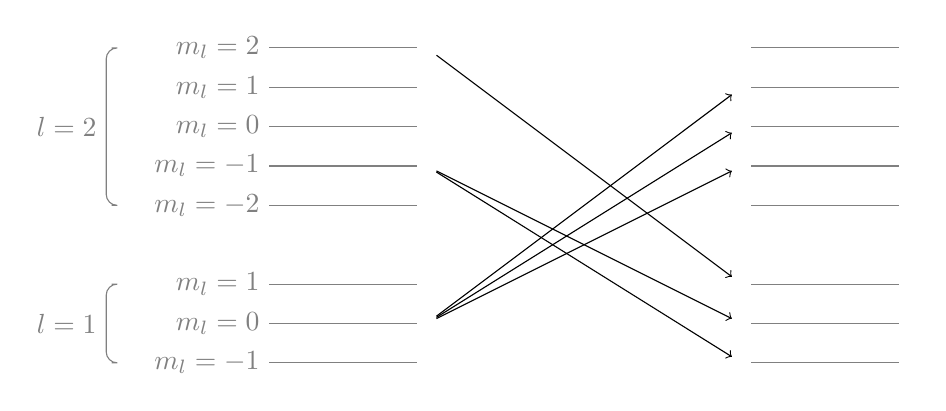
\begin{tikzpicture}
		% Sinistra
		\node (l1-1) at (-2,-1.5){};
		\node (l10)  at (-2,-1)  {};
		\node (l11)  at (-2,-0.5){};
		\node (l2-2) at (-2,0.5) {};
		\node (l2-1) at (-2,1)   {};
		\node (l20)  at (-2,1.5) {};
		\node (l21)  at (-2,2)   {};
		\node (l22)  at (-2,2.5) {};
		% Destra
		\node (r1-1) at (2,-1.5){};
		\node (r10)  at (2,-1)  {};
		\node (r11)  at (2,-0.5){};
		\node (r2-2) at (2,0.5) {};
		\node (r2-1) at (2,1)   {};
		\node (r20)  at (2,1.5) {};
		\node (r21)  at (2,2)   {};
		\node (r22)  at (2,2.5) {};
		% Raggruppamento delle linee con stesso n. quantico l
		\draw[rounded corners,black!50!white] (l1-1) ++(-4,0) -- ++(-2pt,0) to node[left]{$l=1$} ++(0,1) -- ++(2pt,0);
		\draw[rounded corners,black!50!white] (l2-2) ++(-4,0) -- ++(-2pt,0) to node[left]{$l=2$} ++(0,2) -- ++(2pt,0);
		% Linee spettrali non perturbate
		\draw[black!50!white] (l1-1) to +(-2,0) node[left]{$m_l=-1$};
		\draw[black!50!white] (l10)  to +(-2,0) node[left]{$m_l=0$};
		\draw[black!50!white] (l11)  to +(-2,0) node[left]{$m_l=1$};
		\draw[black!50!white] (l2-2) to +(-2,0) node[left]{$m_l=-2$};
		\draw[black!50!white] (l2-1) to +(-2,0) node[left]{$m_l=-1$};
		\draw[black!50!white] (l20)  to +(-2,0) node[left]{$m_l=0$};
		\draw[black!50!white] (l21)  to +(-2,0) node[left]{$m_l=1$};
		\draw[black!50!white] (l22)  to +(-2,0) node[left]{$m_l=2$};
		% Linee spettrali perturbate
		\draw[black!50!white] (r1-1) to +(2,0) node[right]{};
		\draw[black!50!white] (r10)  to +(2,0) node[right]{};
		\draw[black!50!white] (r11)  to +(2,0) node[right]{};
		\draw[black!50!white] (r2-2) to +(2,0) node[right]{};
		\draw[black!50!white] (r2-1) to +(2,0) node[right]{};
		\draw[black!50!white] (r20)  to +(2,0) node[right]{};
		\draw[black!50!white] (r21)  to +(2,0) node[right]{};
		\draw[black!50!white] (r22)  to +(2,0) node[right]{};
		% Frecce per indicare le transizioni tra i livelli
		\draw[thin,black,->] (l22) -- (r11);

		\draw[thin,black,->] (l2-1) -- (r10);
		\draw[thin,black,->] (l2-1) -- (r1-1);

		\draw[thin,black,->] (l10) -- (r21);
		\draw[thin,black,->] (l10) -- (r20);
		\draw[thin,black,->] (l10) -- (r2-1);
	\end{tikzpicture}
	\caption{Esempio della divisione di alcune linee spettrali dovuta all'effetto Zeeman normale.}
	\label{fig:zeeman-normale}
\end{figure}

Le transizioni tra livelli di energia di $\op H^{(0)}$ sono, come visto nel capitolo precedente, permesse solo se $\Delta l=\pm 1$ e $\Delta m_l=0,\pm 1$, quindi la variazione di energia tra i livelli perturbati è
\begin{equation}
	\Delta H=\Delta E^{(0)}+\frac{e\hbar B}{2mc}\Delta m_l
\end{equation}
da cui si nota che dove prima si aveva un livello, ora in corrispondenza ne osserviamo tre.
In realtà le osservazioni sperimentali mostrano che questa descrizione è sbagliata: si sono misurate più di tre linee anche non equidistanti tra loro.
Si è scoperto infatti che l'elettrone, come le altre particelle elementari, possiede un altro tipo di momento angolare, detto \emph{momento angolare intrinseco} o \emph{spin}, di cui non si è tenuto conto in queste equazioni.

\chapter{Sistemi con più gradi di libertà}
Salvo brevi eccezioni, finora abbiamo trattato solamente dei sistemi ad un grado di libertà, tipicamente una particella in moto lungo una retta.
Passiamo ora a studiare sistemi con più gradi di libertà, che possono corrispondere ad un maggior numero di particelle, all'aggiunta di altre dimensioni spaziali, o entrambe.
In questo capitolo ci occuperemo di introdurre lo schema matematico in cui inquadrare questi problemi, in via generale, per poterlo poi applicare a problemi più complessi di quelli già visti, come le rotazioni e gli atomi.

\section{Prodotto diretto di spazi vettoriali}
Il problema principale è capire come costruire lo spazio degli stati di tali sistemi.
Sappiamo che con un grado di libertà possiamo associare ad ogni stato un raggio in uno spazio di Hilbert complesso, separabile e infinito dimensionale.
Quando il sistema possiede più di una dimensione spaziale, tali dimensioni sono indipendenti e apportano ciascuna un grado di libertà; per ciascuna di esse abbiamo, ad esempio, un operatore della posizione e uno dell'impulso, e sappiamo già dai commutatori fondamentali che posizione e impulso di coordinate differenti commutano.
Analogamente, componendo più particelle in un sistema ciascuna di esse ha associata la coppia di operatori posizione e impulso (ad esempio) e tutti quelli che ne derivano.
/bin/bash: :wq: command not found
\begin{equation}
	\hilbert=\hilbert_1\otimes\hilbert_2\otimes\cdots\otimes\hilbert_d.
\end{equation}

Per studiare la definizione e le proprietà di base ci restringiamo ora al prodotto di due spazi $\hilbert_1$ e $\hilbert_2$.
Dati gli stati (qualsiasi) $\ket{A}\in\hilbert_1$ e $\ket{B}\in\hilbert_2$, possiamo costruire il loro prodotto diretto $\ket{A}\otimes\ket{B}$ che rappresenta lo stato del sistema combinato $\hilbert=\hilbert_1\otimes\hilbert_2$ in cui il sottosistema $\hilbert_1$ è nello stato $\ket{A}$ e il sottosistema $\hilbert_2$ è nello stato $\ket{B}$.
Chiaramente il prodotto non è commutativo, perch\'e in generale non è detto nemmeno che esista uno stato $\ket{A}$ in $\hilbert_2$ in modo da poter scrivere $\ket{B}\otimes\ket{A}$.
Lo spazio vettoriale $\hilbert_1\otimes\hilbert_2$ è dotato in modo naturale delle operazioni di somma e di moltiplicazione per scalare (un numero complesso) esattamente come gli spazi di partenza: esso contiene le coppie $\ket{A}\otimes\ket{B}$ per \emph{ogni} stato $\ket{A}\in\hilbert_1$ e ogni stato $\ket{B}\in\hilbert_2$, e tutte le possibili combinazioni lineari di essi.
Il \textit{bra} associato al \textit{ket} $\ket{A}\otimes\ket{B}$ è semplicemente $\bra{A}\otimes\bra{B}$; con questo, il prodotto interno nello spazio prodotto è definito come
\begin{equation}
	(\bra{A}\otimes\bra{B})(\ket{C}\otimes\ket{D})=\braket{A}{C}\braket{B}{D}
\end{equation}
che, in termini di probabilità, mostra come gli ``eventi'' nei due sistemi siano indipendenti, poich\'e la probabilità dell'evento composto risulta essere il prodotto delle singole probabilità.
Spesso lo stato composto si scrive omettendo il simbolo $\otimes$, o anche in un unico \textit{ket}, come
\begin{equation}
	\ket{A}\otimes\ket{B}\hspace{2cm}\ket{A}\ket{B}\hspace{2cm}\ket{A,B}.
\end{equation}
Utilizzeremo per un po' la prima e la terza notazione insieme.

Anche se possiamo costruire uno stato composto dal prodotto di due stati, non è vero che ogni stato del sistema composto si possa scrivere in tale modo: in generale, uno stato $\ket{\psi}\in\hilbert=\hilbert_1\otimes\hilbert_2$ è una combinazione lineare di stati composti.
Date due basi di autostati (eventualmente anche continui) $\ket{i}$ e $\ket{j}$ per gli spazi, una base dello spazio prodotto è l'insieme $\{\ket{i}\otimes\ket{j}=\ket{i,j}\}$, quindi in generale
\begin{equation}
	\hilbert\ni\ket{\psi}=\sum_{i,j}c_{ij}\ket{i,j}=\sum_{i,j}c_{ij}\ket{i}\otimes\ket{j}
\end{equation}
dove come al solito $c_{ij}=\braket{i,j}{\psi}=(\bra{i}\otimes\bra{j})\ket{\psi}$.
Solo nel caso in cui $c_{ij}$ si può scrivere nella forma $a_ib_j$ allora si ha
\begin{equation}
	\ket{\psi}=\sum_{i,j}a_ib_j\ket{i,j}=\sum_{i,j}a_i\ket{i}\otimes b_j\ket{j}=\bigg(\sum_ia_i\ket{i}\bigg)\otimes\bigg(\sum_jb_j\ket{j}\bigg)
\end{equation}
cioè $\ket{\psi}$ si può scrivere come prodotto di due stati semplici, e si dice talvolta \emph{separabile}.
Quando non esiste una tale fattorizzazione, lo stato è detto \emph{entangled}.\footnote{
	Letteralmente \textit{ingrovigliato}, \textit{intrecciato}.
	Il termine inglese è di uso comune, e raramente si trova tradotto in italiano.
}



\backmatter

% Bibliografia
\cleardoublepage
\phantomsection
\addcontentsline{toc}{part}{\bibname}
\nocite{*}
\printbibliography

% Indice
\cleardoublepage
\pdfbookmark[-1]{Indice}{contents}
\tableofcontents
\end{document}
